% PREAMBLE 
%\documentclass[9pt,lineno]{elife}
\documentclass[custompaper]{MBE}%
%\DeclareOption{a4paper}
\usepackage{url}
\usepackage{xcolor}
\usepackage{subcaption}
\usepackage{hyperref}
\hypersetup{
    colorlinks=true,
    linkcolor=blue,
    filecolor=magenta,      
    urlcolor=cyan,
}

\newcommand{\sgcomment}[1]{\textcolor{blue}{SG: #1}}
\newcommand{\luke}[1]{\textcolor{blue}{Luke: #1}}
\newcommand{\logit}{\operatorname{logit}}

%\jshort{mst}

%\volname{}

%\jvolume{0}

%\jvol{}

%\jissue{0}

%\pubyear{2019}

\mstype{Article}

%\artid{012}

%\access{Advance Access publication March 3, 2013}

\begin{document}

\keyword{1000 Genomes Project, Batch Effect, Population Structure, GWAS, GCAT}

\title{\ Legacy Data Confounds Genomics Studies}

\author[Anderson-Trocm\'e et al.]{\ Luke \surname{Anderson-Trocm\'e},$^{\ast,1,2}$ Rick Farouni,$^{1,2}$ Mathieu Bourgey,$^{1,2}$ Fumihiko Matsuda,$^{3}$, Yoichiro Kamatani$^{3}$, and Simon Gravel$^{1,2}$,}

\address{$^{1}$Department of Human Genetics, McGill University, Montreal, QC H3A 0G1, Canada\\
$^{2}$McGill University and Genome Quebec Innovation Centre, Montreal, QC H3A 0G1, Canada\\ 
$^{3}$Center for Genomic Medicine, Graduate School of Medicine, Kyoto University, Kyoto 606-8501, Japan}

\coresp{simon.gravel@mcgill.ca}

\abstract{Recent reports have identified differences in the mutational spectra across human populations. While some of these reports have been replicated in other cohorts, most have been reported only in the 1000 Genomes Project (1kGP) data. While investigating an intriguing putative population stratification within the Japanese population, we identified a previously unreported batch effect leading to spurious mutation calls in the 1kGP data and to the apparent population stratification. Because the 1kGP data is used extensively, we find that the batch effects also lead to incorrect imputation by leading imputation servers and suspicious GWAS associations. Lower-quality data from the early phases of the 1kGP thus contaminates modern studies in hidden ways, and a community effort may be required to remove or upgrade such legacy sequencing data from reference databases. }

\maketitle

\section{Introduction}
	
\subsection{Batch Effects in Aging Reference Cohort Data}			

The last 5 years have seen a drastic increase in the amount and quality of human genome sequence data. 
Reference cohorts such as the International HapMap Project \citep{HapMap2005}, the 1000 Genomes Project (1kGP)\citep{1000GenomesProjectConsortium2010,The1000GenomesProjectConsortium2012,phase3}, and the Simons Diversity project \citep{Mallick2016}, for example, have made thousands of genome sequences publicly available for population and medical genetic analyses. 
Many more genomes are available indirectly through servers providing imputation services \citep{HapMap2005} or summary statistics for variant frequency estimation \citep{Lek2016}.

The first genomes in the 1kGP were sequenced 10 years ago \citep{VanDijk2014}. Since then, sequencing platforms have rapidly improved.  
The second phase of the 1kGP implemented multiple technological and analytical improvements over its earlier phases \citep{The1000GenomesProjectConsortium2012,phase3}, leading to heterogeneous sample preparations and data quality.

Yet, because of the extraordinary value of freely available data, early data from the 1kGP is still widely used as a reference panel for imputation, allele frequency estimations and to answer a wide range of medical and evolutionary questions.
This raises the question of whether and how such legacy data should be included in contemporary analyses alongside more recent cohorts.
Here we point out how large and previously unreported batch effects in the early phases of the 1kGP still lead to incorrect genetic conclusions through population genetic analyses and spurious GWAS associations as a result of imputation using the 1kGP as a reference.

\subsection{Mutational Signatures}

Different mutagenic processes may preferentially affect different DNA motifs. 
Certain mutagens in tobacco smoke, for example, have been shown to preferentially bind to certain genomic motifs leading to an excess of G to T transversions \citep{Pfeifer2002,Pleasance2010}. 
Thus, exposure of populations to different mutational processes can be inferred by considering the DNA context of polymorphism in search of \textit{signatures} of different mutational processes \citep{Alexandrov2013,Shiraishi2015a}. 
Such genome-wide mutational signatures have been used as diagnostic tools for cancers (e.g., \cite{Alexandrov2013,Shiraishi2015a}).

In addition to somatic mutational signatures, there has been recent interest in population variation in germline mutational signatures which can be revealed in large sequencing panels. 
In 2015, Harris reported 50\% more TCC ${\rightarrow}$ TTC mutations in European populations compared to African populations, and this was replicated in a different cohort in 2017 \citep{Harris2015a, Harris2017a, Mathieson2017a}. 
Strong population enrichments of a mutational signature suggests important genetic or environmental differences in the history of each population \citep{Harris2015a, Harris2017a}. 
Harris and Pritchard further identified distinct mutational spectra across a range of populations, which were further examined in a recent publication by Aikens et al. \citep{Harris2017a,Aikens2018}.
 
In particular, the latter two studies  identified a heterogeneous mutational signature within 1000 Genomes Japanese individuals.
This heterogeneity is intriguing because differences in germline signatures accumulate over many generations.
A systematic difference within the Japanese population would suggest sustained environmental or genetic differences across sub-populations within Japan with little to no gene flow.
We therefore decided to follow up on this observation, by using a newly sequenced dataset of Japanese individuals. 

While we were unable to reproduce the mutational heterogeneity within the Japanese population, we could trace back the source of the discrepancy to a technical artefact in the 1kGP data.
In addition to creating biases in mutational signatures, this artefact leads to spurious imputation results which have found their way in a number of recent publications.


The results section is organized as follows.
We first attempt to reproduce the original signal and identify problematic variants in the JPT cohort from the 1kGP. 
Next, we expand our analysis to the other populations in the 1kGP and identify lists of variants that show evidence for technical bias.
Finally, we investigate how these variants have impacted modern genomics analyses.  
  

\begin{figure}
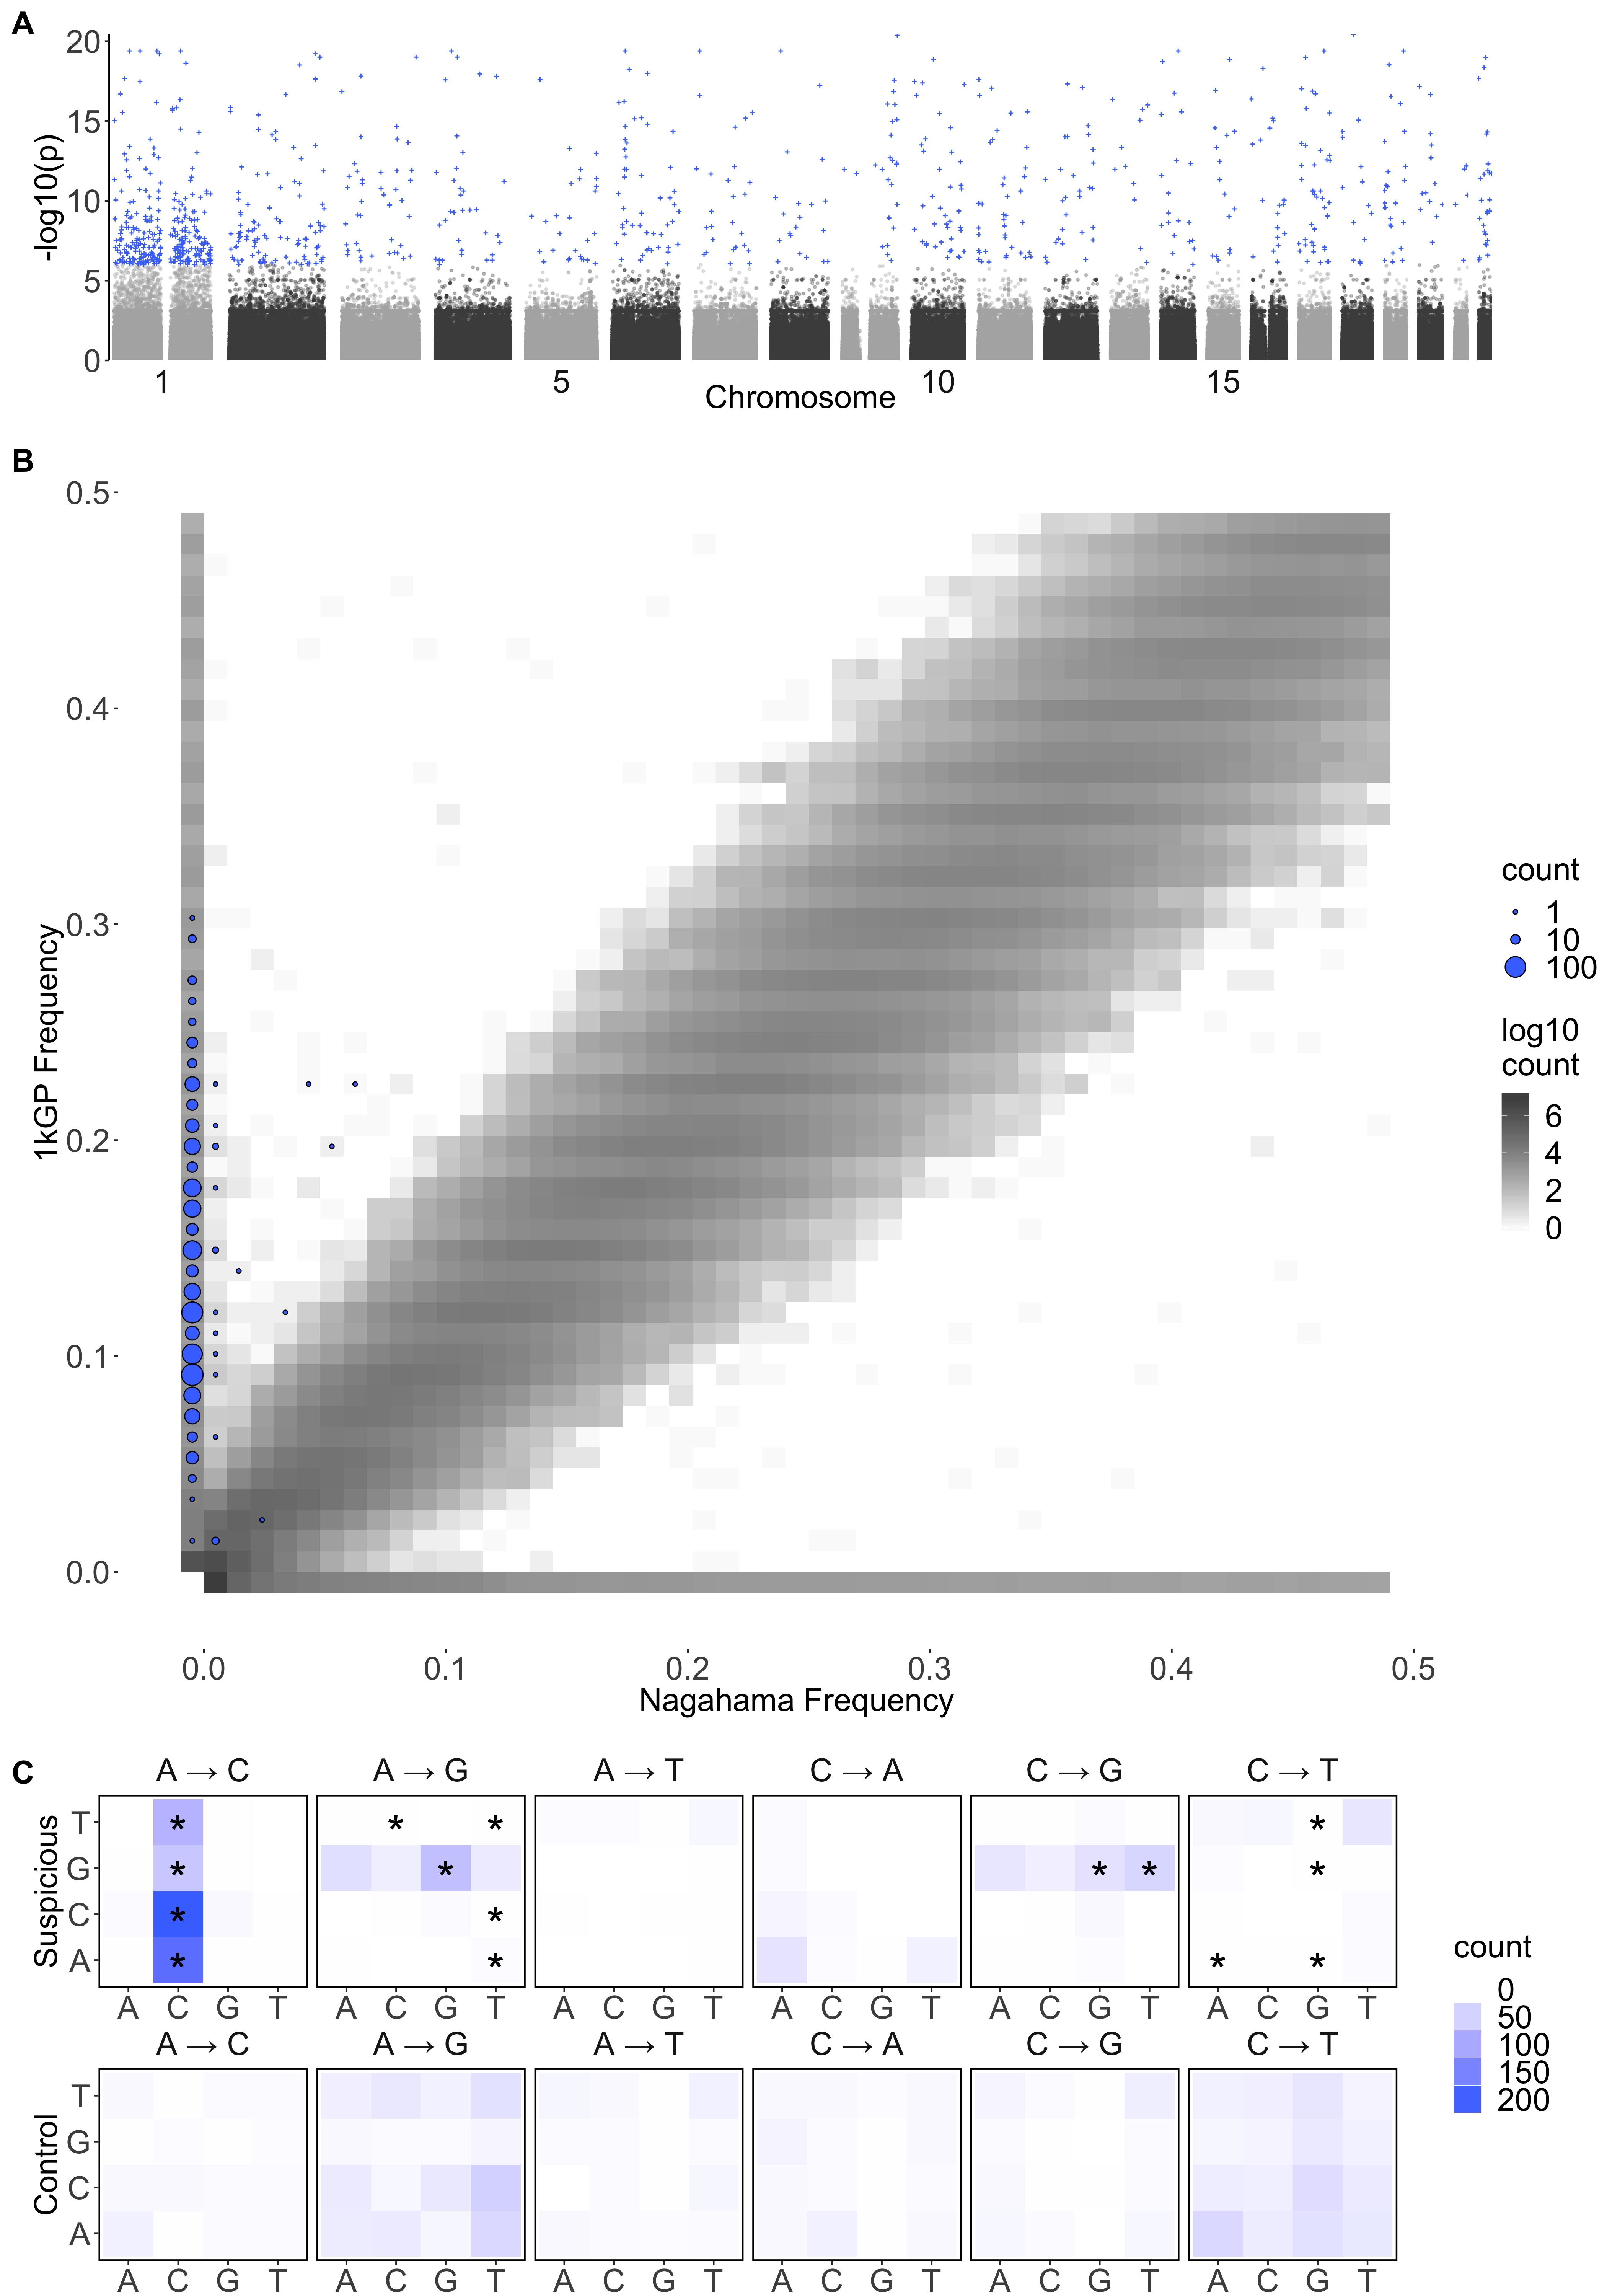
\includegraphics[width=\hsize,keepaspectratio]{./Figures/Figure1.jpg}
\caption{
\textbf{A} 
Mutation spectrum of the 1034 variants that reached a genome wide significance with a \textit{p}-value less than $p < 10^{-6}$  in a GWAS of sequencing quality. 
The majority of the variants with significant associations to $Q$ have the *AC${\rightarrow}$*CC mutational pattern. There is also a slight enrichment in GA*${\rightarrow}$GG* and GC*${\rightarrow}$GG* mutations. These three enrichments can be summarized as G**${\rightarrow}$GG*. (note: the reverse complement of *AC${\rightarrow}$*CC is GT*${\rightarrow}$GG*)
\textbf{B} 
Joint frequency spectrum plot of the Japanese from the 1kGP and a more recent Nagahama dataset.
Crosses ( + ) are variants that reached genome wide significance in a GWAS of sequencing quality. 
The histogram on the left of the plot is the distribution of significant variants. 
\textbf{C} 
Genome wide association of the average quality of mapped bases $Q$ for the 104 Japanese individuals included in the 1kGP. This GWAS identified $587\ \  p < 10^{-8}$ and $1034\ \ p < 10^{-6}$ SNPs that were associated to the average $Q$ of SNPs mapped for an individual
The same analysis was performed independently for each of the populations in the 1kGP. }
 \label{SFS}
\end{figure}


\section{Results}

			
\subsection{A peculiar mutational signature in Japan}			
	
Harris and Pritchard reported an excess of a 3-mer substitution patterns *AC${\rightarrow}$*CC in a portion of the Japanese individuals in the 1kGP \citep{Harris2017a}.
While trying to follow up on this observation in a larger and more recent Japanese cohort, we did not find this particular signature.
When comparing the allele frequencies between the Japanese individuals from the 1kGP and this larger dataset, we observed a number of single nucleotide polymorphisms (SNPs) private to one of the two groups (Figure \ref{SFS}).
Given the similarity of the two populations, this strongly suggests a technical difference rather than a population structure effect.
These mismatches were present despite filtering for low-quality regions of the human genome and Hardy-Weinberg disequilibrium. 

When mismatch sites are removed from the 1kGP data, the  *AC${\rightarrow}$*CC signal disappears (Figure \ref{SFS}). To identify possible technical reasons for the difference, we performed regressions of the prevalence of the  *AC${\rightarrow}$*CC mutational signature against different individual-level quality metrics provided by the 1kGP (see Supplementary Figure \ref{PC1_Correlation}). 
The average quality of mapped bases  $Q$ per individual stood out as a strong correlate : Individuals with low $Q$ show elevated rates of the signature. 
Thus, sequences called from low-$Q$ data contain variants that reproduce poorly across studies and exhibit a particular mutational signature. 

\begin{figure}
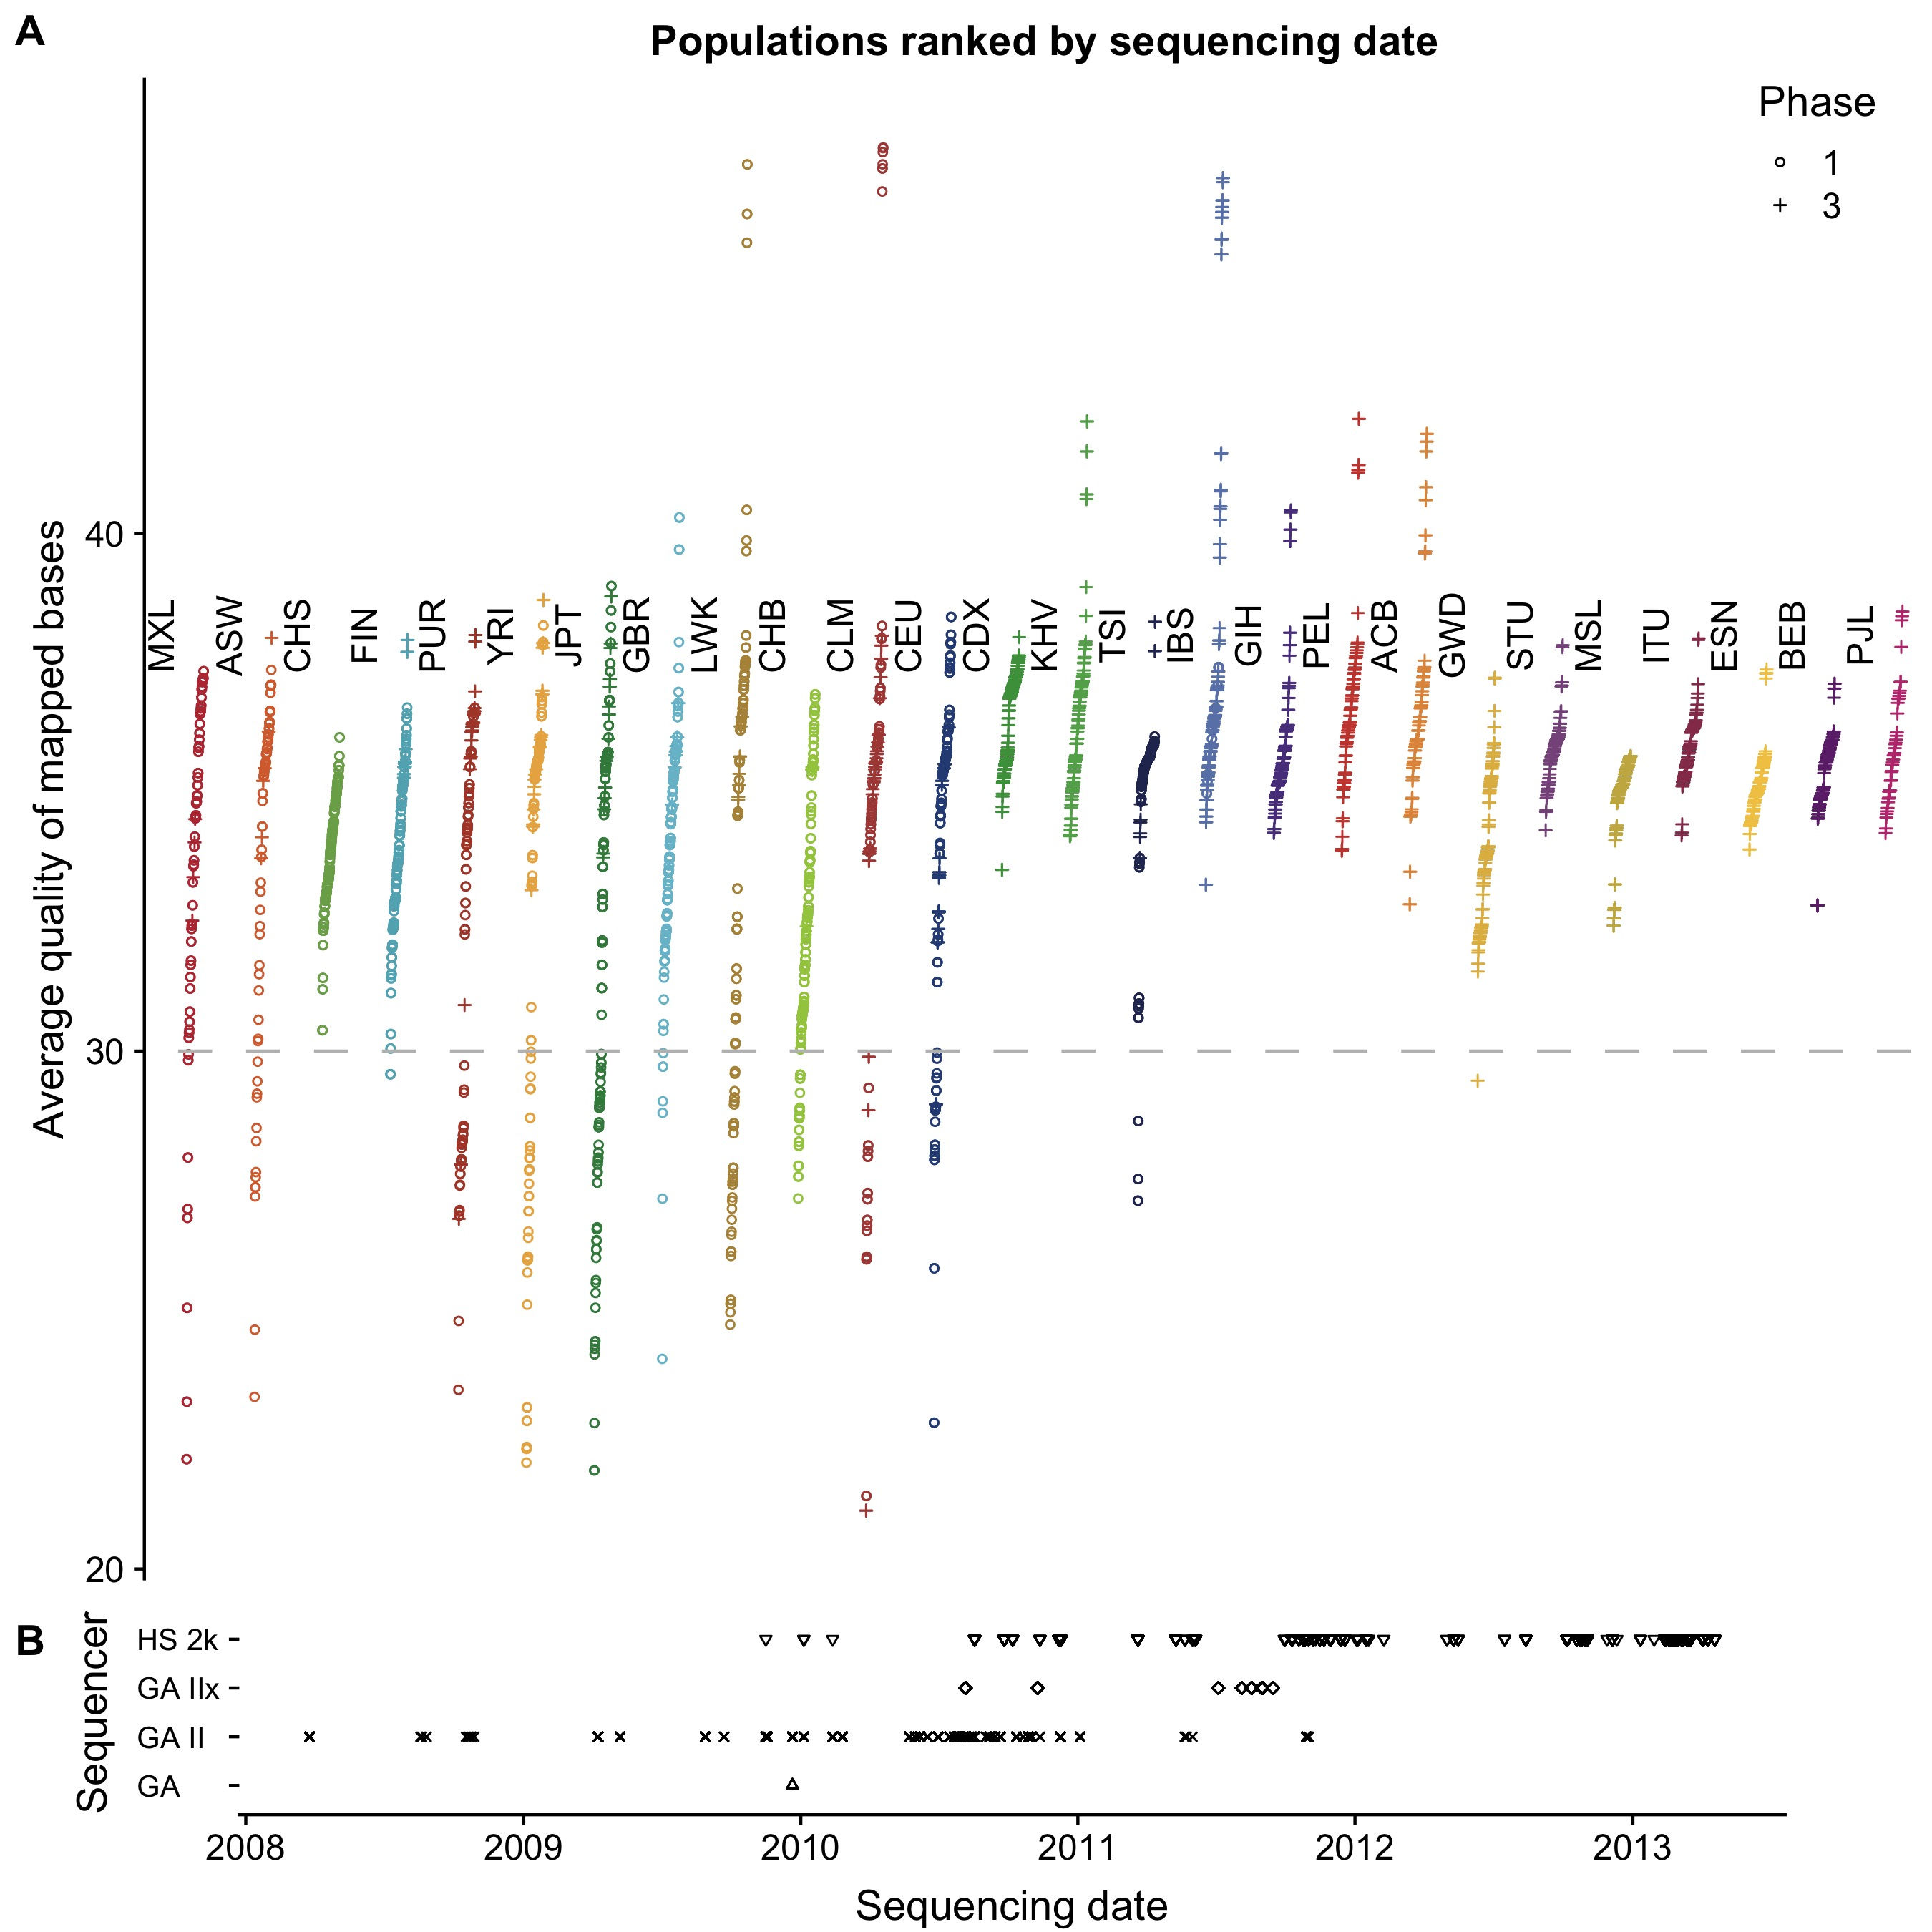
\includegraphics[width=0.95\hsize,keepaspectratio]{./Figures/MapQualOverTime.jpg}

\caption{\textbf{A} The average quality of mapped bases $Q$ for each individual per population included in the 1000 Genomes sequencing project. Individuals are ranked by the date of the earliest sequencing data is used for individuals sequenced more than once. The x-axis is ranked by the mean sequencing date per population. \textbf{B} The x-axis is sorted by the sequencing date per individual. The colours indicate the sequencing centres that produced the data for each individual and the shape indicates whether the individual belongs to Phase 1 or Phase 3 of the 1000 Genomes project. The bottom plot indicates the sequencing technologies used over time.}
\label{MapQual}
\end{figure}

To identify SNPs that are likely to reproduce poorly across cohorts without having access to a second cohort, we performed an association study in the JPT for SNPs that associate strongly with low $Q$ (Figure \ref{SFS}).
Traditionally, genome wide association studies use genotypes as the independent variable. 
Here we perform a ``reverse GWAS'' or Genotype-Conditional Association Test, in the sense that genotypes are now the dependent variable that we attempt to predict using the continuous variable $Q$ as the independent variable \citep{song2015testing}.
We use logistic regression of the genotypes on $Q$ and identify 587 SNPs with $p < 10^{-8}$ and 1034 SNPs with $ p < 10^{-6}$. 
While identifying putative low-quality SNPs to exclude, using a higher $p$-value threshold increases the stringency of the filtering (i.e., excluding SNPs with $ p < 10^{-6}$ is more stringent than excluding SNPS with $p < 10^{-8}$). 
The variants that are associated to $Q$ have an enrichment in *AC${\rightarrow}$*CC mutations, GA*${\rightarrow}$GG*, and GC*${\rightarrow}$GG* mutations (Figure \ref{SFS}A).
These three enrichments can be summarized as an excess of G**${\rightarrow}$GG* in individuals with low $Q$.

Thus, this mutational signal is heavily enriched in suspicious SNPs, but residual signal remains in non-significant SNPs, presumably because many rare alleles found in individuals with low $Q$ remain unidentifiable using association techniques (Figure \ref{MutSpect}). The removal of individuals with $Q$ below 30 successfully removes the *AC${\rightarrow}$*CC signal, however other signals identified by Harris and Pritchard appear unchanged (Figure \ref{MutSpect}).
For population genetic analyses sensitive to the accumulation of rare variants, the removal of individuals with low $Q$ appears preferable to filtering specific low-quality SNPs. 
For other analyses where quality of imputation matters, identifying suspicious variants may be preferable. 


\subsection{Identifying suspicious variants in the 1kGP}
The distribution of $Q$ across 1kGP populations shows that many populations have distributions of $Q$ scores comparable to that of the JPT, especially populations sequenced in the phase 1 of the project: sequencing done in the early phases of the 1kGP was more variable and overall tended to include lower quality sequencing data (Figure \ref{MapQual}).
This variability could result from evolving sequence platform and protocols or variation between sequencing centres. 
By 2011, older sequencing technologies were phased out, and methods became more consistent, resulting in higher and more uniform quality.


We therefore performed the same reverse GWAS approach in all populations independently, and similarly identified $Q$-associated SNPs in 24 of the 26 populations in the 1kGP, with the phase 1 populations being most affected, with on average four times as many significantly associated sites compared to the phase 3 populations.
Over 3,826 variants were independently associated to low $Q$ in at least two populations with $ p < 10^{-6}$ in each (Figure \ref{OverLap}).

To build a test statistic to represent the association across all populations simultaneously, we performed a simple logistic regression predicting genotype based on $Q$ with the logistic factor analysis (LFA) as an offset to account for population structure or Genotype-Conditional Association Test  (GCAT) as proposed by \citep{song2015testing}. 
We also considered two alternative approaches to account for confounders, namely using the leading five  principal component analysis, and using population labels as covariates (Supplementary Figure \ref{CompareModel}). 

This method identifies a total of 24,390 variants associated to $Q$ (Figures \ref{NRS_Manhattan},\ref{NRI_Manhattan}, \ref{RS_Manhattan}, and \ref{RI_Manhattan}). 
To account for the large number of tests, we used a two-stage Benjamini \& Hochberg step-up FDR-controlling procedure to adjust the p-values using a nominal Type-I error rate $\alpha = 0.01$ \citep{Benjamini2006}. 
We tested SNPs, INDELs and repetitive regions separately as they may have different error rates (Table \ref{sigTable}).
Lists of suspicious variants and individuals with low $Q$ are provided as supplementary material \ref{rsIDList}.


\begin{table}
\centering
\begin{tabular}{l  r r}
                      & {Repeat}  & {Non-Repeat}       \\ \hline
{SNP}  & 5,186 & 17,124 \\  
{INDEL} & 509 & 1,571 \\ \hline
\end{tabular}
\caption{Number of statistically significant variants per category. 
Variants that are flagged by the 1kGP nested repeat mask file were analyzed separately. 
SNPs and INDELs were also analyzed separately. 
The total number of 24,390 are statistically significantly associated to $Q$.}
\label{sigTable}
\end{table}

\begin{figure}
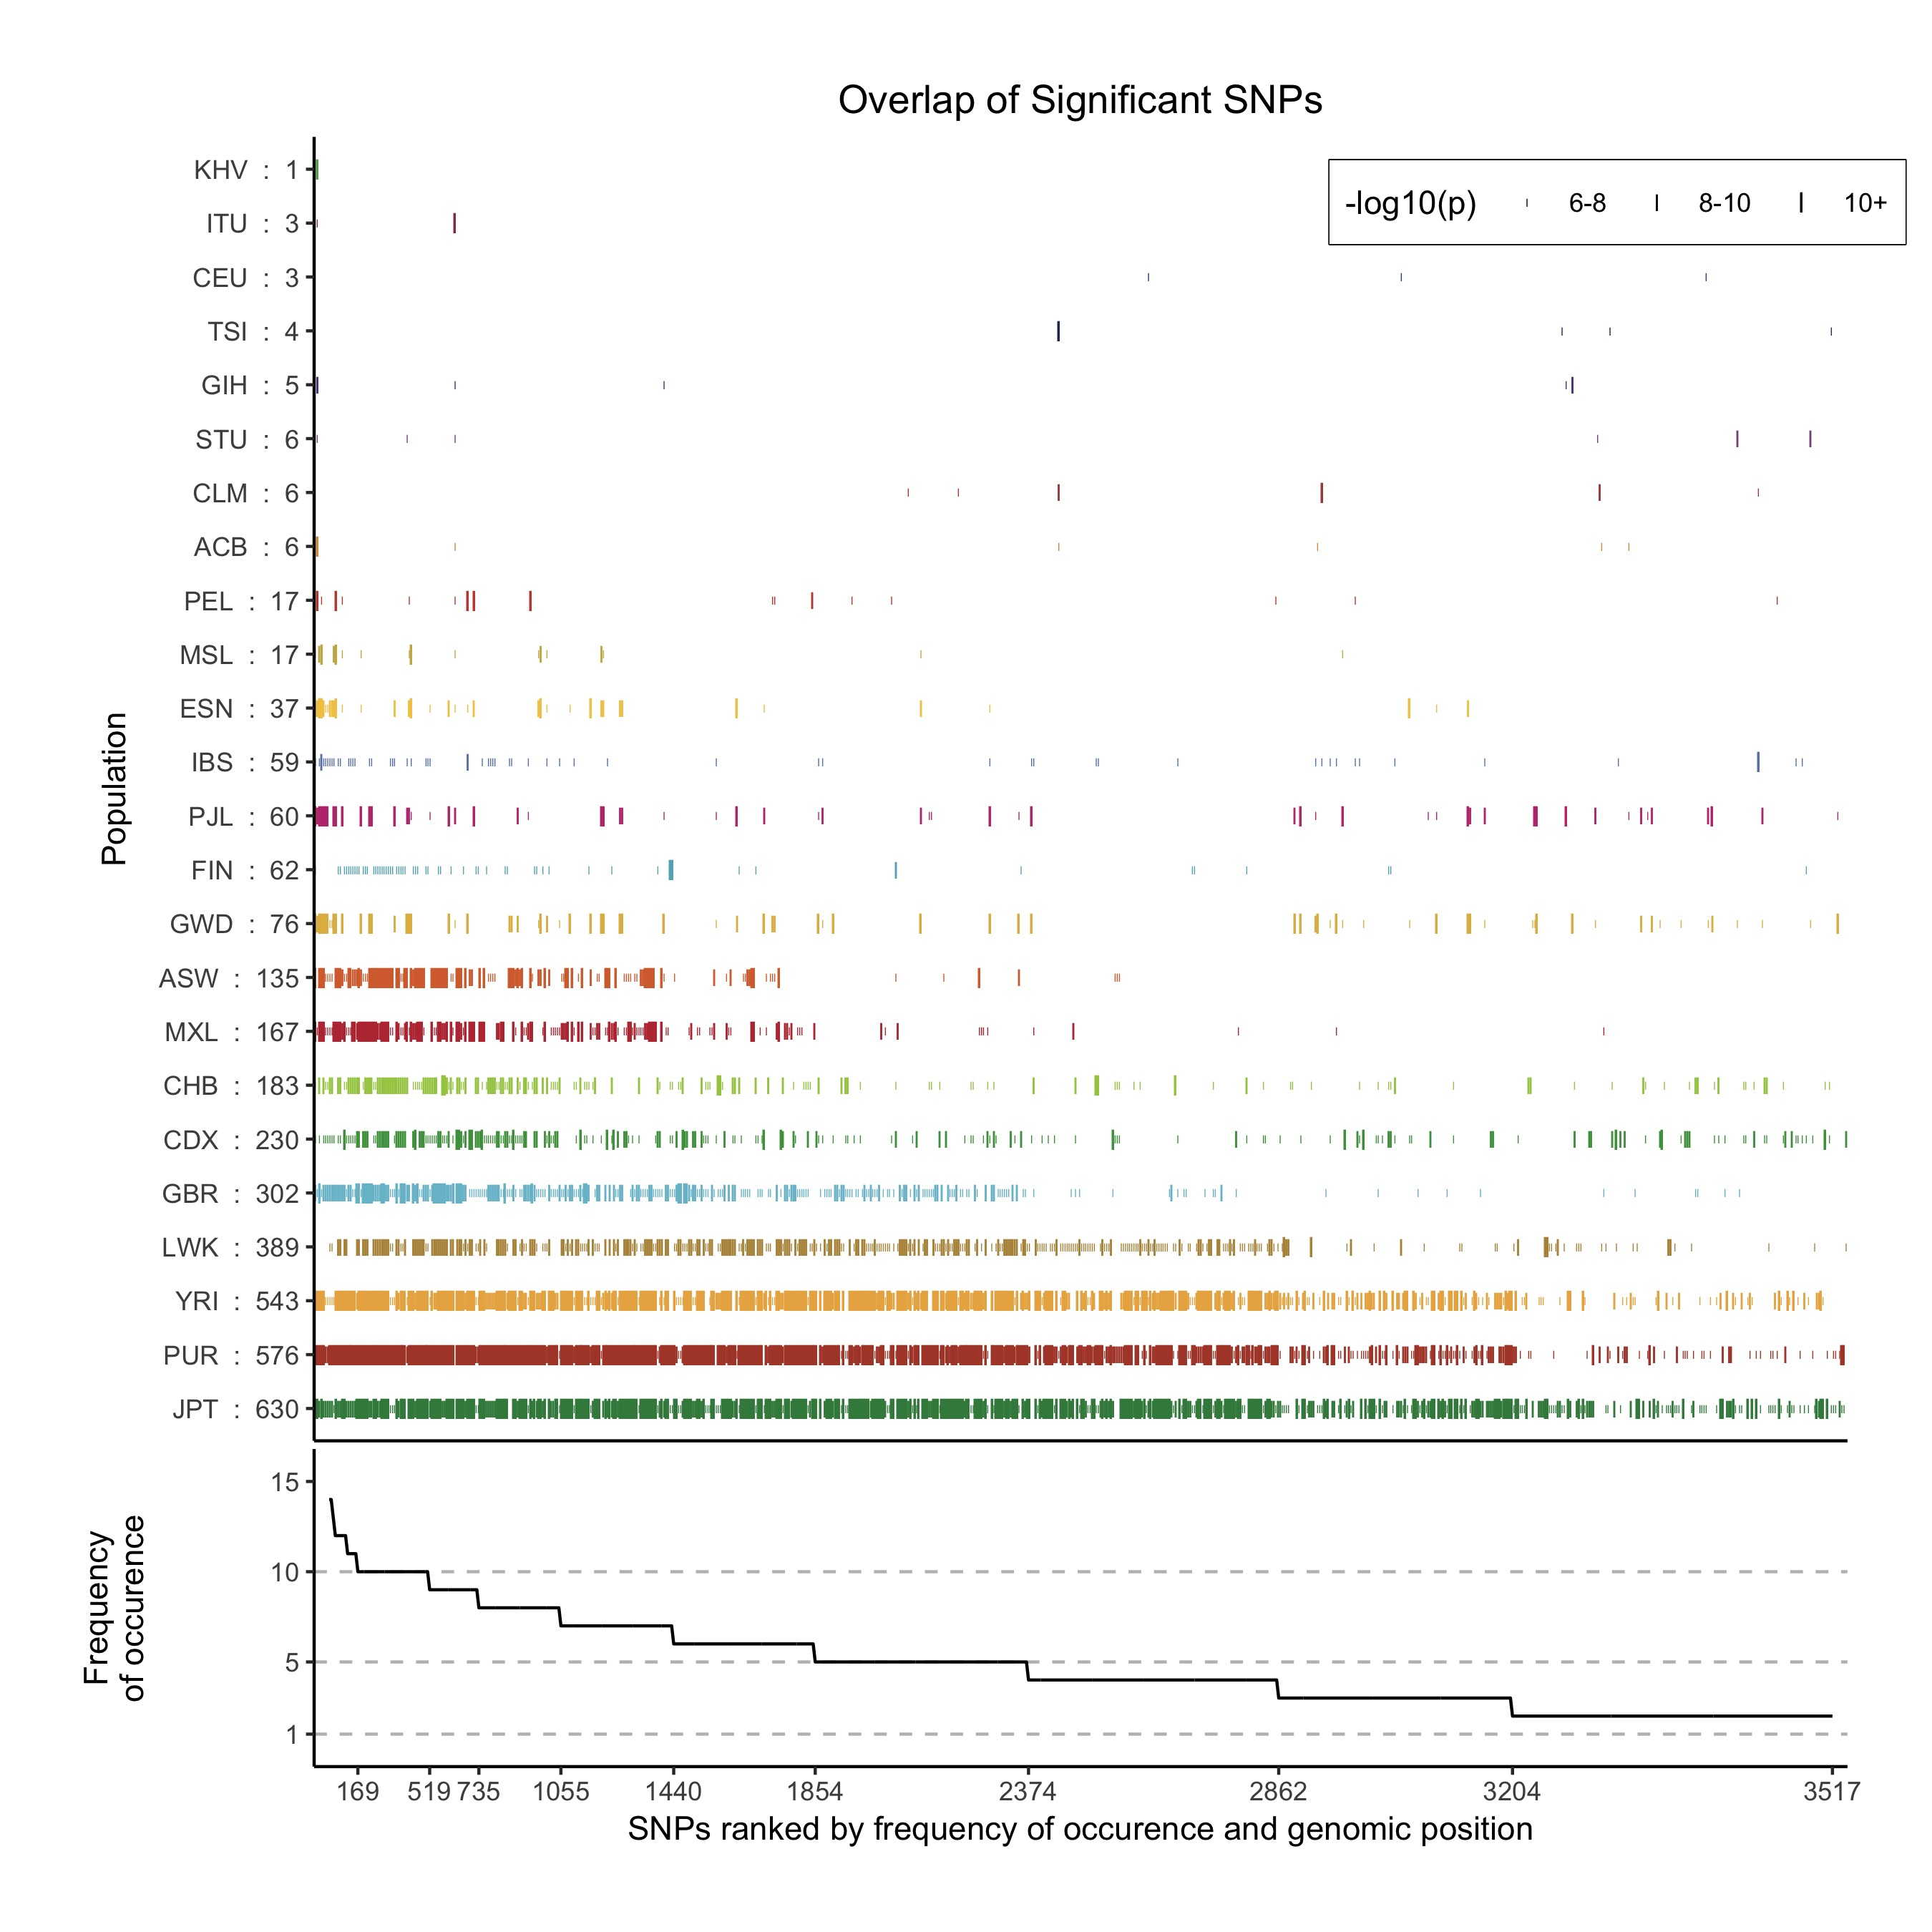
\includegraphics[width=\hsize,keepaspectratio]{./Figures/SNPOverlap6.jpg}

\caption{Variants associated with average quality of mapped bases $Q$ in more than one population.
The size of the crosses ( + ) are proportional to the -log10(p) value of that SNP.
The x axis is ranked by the frequency of occurrence of a SNP, then by genomic position.
Phase 1 populations are marked by a star ( * ).
The line plot underneath shows the number of populations for which a variant has reached significance.
The populations that tend to have the most individuals with low $Q$ also tend to have the most variants associated to $Q$. 
The same variants identified as being low quality independently in each population are found in other populations. }
  \label{OverLap}
\end{figure}
To ensure that population structure was properly taken into account, we considered alternative models with principal components (PCs), Population membership or both as a covariate. 
These models were broadly consistent (See Figure \ref{CompareModel}).

\subsection{Cell line or technical artifact}

In 2017, Lan et al. resequenced 83 Han Chinese individuals from the 1kGP \citep{Lan2017}.
After restricting the analysis to individuals present in both datasets, we find 296 suspicious variants polymorphic in 1kGP. Of those, 9 are present in the resequenced data \ref{90HanSFS}.
While this provides strong validation that the variants are not cell-line specific mutations, it is more than the 0.1\% of the sites: some variants that are associated to $Q$ may be present in the population but have biased genotypes.

We did a similar analysis using the variants identified in the GCAT model present in the 83 resequenced individuals.
Of the 24,390 suspicious variants identified globally, only 12,086 of them are found in the 83 individuals in the original 1kGP data (See Figure \ref{90HanSFS_full}).
From this subset, only 1,637 of these variants are present in the resequenced data, the rest are missing entirely.
Figure \ref{90HanSFS_full} shows a relatively weak correlation to allele frequency for the variants present in the resequenced data.
A number of variants shared across cohorts suggests that roughly 10\% of the variants identified are present in the cell lines real but exhibit genotyping bias.


We found that 613 of the variants we identified as being associated to $Q$ were present on Illumina's Omni 2.5 chip. 
This does not mean that these variants are false positives, but rather, that in the 1kGP, individuals with low $Q$ were less likely to be called as having a variant in that position. 
Moreover, using the 1kGP as a reference panel might impact the population allele frequencies observed for these positions.

\subsection{Suspicious variants impact modern genomics analyses}

State of the art imputation servers use a combination of many databases including some that are not freely available.
From the perspective of researchers, they act as black-box imputation machines that take observed genotypes as input and return imputed genotypes.  

To investigate the proportion of suspicious variants that are being imputed, we submitted the first two chromosomes of  the 1kGP genotype data to the Michigan Imputation Server.
We found that all of the variants associated with $Q$ were imputed back in the samples.
This suggests that the imputation reference panel still includes individuals with low $Q$, and the dubious variants will be imputed in individuals who most closely match the low-quality individual.

We searched the literature for any GWAS that might have reported these dubious variants as being significantly associated with some biological trait, even though there is no particular reason for these variants to be associated with phenotypes.
The NHGRI-EBI Catalog of published genome-wide association studies identified seventeen recent publications that had reported these variants as close to or above the genome-wide significant threshold (Table \ref{gwasTable}).

Eleven of these studies included the 1kGP in their reference panel for imputation \citep{xu2012genome, lutz2015genome, park2015mercapturic, astle2016allelic, herold2016family,  suhre2017connecting, lopez2017genome, tian2017genome,  spracklen2017association,  nagy2017exploration, gao2018genome} and another used the 1kGP sequence data and cell lines directly \citep{Mandage2017}.
One study used an in-house reference panel for imputation \citep{nishida2018key}, two studies genotyped individuals and imputed the data using the HapMap II as a reference  database for imputation \citep{Kraja2011, Ebejer2013} and two studies used chip sequence data \citep{yucesoy2015genome, ellinghaus2016analysis}.

All papers used a variety of strict quality filters, including Hardy-Weinberg equilibrium test, deviations in expected allele frequency and sequencing data quality thresholds.
They also removed rare alleles and alleles with high degrees of missingness.
Despite using state-of-the-art quality controls, these variants managed not only to be imputed onto real genotype data, but they also reached genome wide significance for association with biological traits.

These associations are not necessarily incorrect -- a weak but significant bias in imputation may still result in a correct associations. To distinguish between weak but significant biases and dubious SNPS, we also considered the effect size and distinguished between variants where the allele frequency difference between low- and high-$Q$ individuals is larger than a factor of two.


\begin{table}[h]
\begin{tabular}{l l l r r r}
  {Pubmed ID}  & {Journal} & {rsID} & \multicolumn{1}{p{1cm}}{\centering GWAS \\ -$\log_{10} p$} & \multicolumn{1}{p{1.5cm}}{\centering $Q$ -$\log_{10} p$\\(adjusted)}      \\ \hline
28654678 & PLoS One & rs201761909 & 5.7 & 78.11\\
	& 	&  	rs201130852 & 5.05 & 72.28\\
	& 	&  	rs201255786 & 5.7 & 68.97\\
	& 	&  	rs200655768 & 6.52 & 66.67\\
	& 	&  	rs184202621 & 5.52 & 60.45\\
	& 	& 	rs80274284 & 6 & 56.15\\
	& 	& 	rs200699422 & 5.3 & 7.43\\
23527680 & \multicolumn{1}{p{3cm}}{\raggedright Twin Research and\\Human Genetics} & rs6057648 & 5.4 & 20.5\\
28928442 & \multicolumn{1}{p{3cm}}{\raggedright Nature Communications} & rs201471471 & 6.52 & 7.87\\
26053186 & \multicolumn{1}{p{3cm}}{\raggedright PLoS One} & rs60136336 & 5.7 & 2.25\\ \hline
\textcolor{gray}{28270201} & \multicolumn{1}{p{3cm}}{\raggedright \textcolor{gray}{Genome Medicine}} & \textcolor{gray}{rs453755} & \textcolor{gray}{7.52} & \textcolor{gray}{5.29}\\
\textcolor{gray}{23023329} & \multicolumn{1}{p{3cm}}{\raggedright \textcolor{gray}{Nature Genetics}} & \textcolor{gray}{rs103294} & \textcolor{gray}{*15.3} & \textcolor{gray}{4.32}\\
\textcolor{gray}{28334899} & \multicolumn{1}{p{3cm}}{\raggedright \textcolor{gray}{Human Molecular Genetics}} & \textcolor{gray}{rs103294} & \textcolor{gray}{*29.3} & \textcolor{gray}{4.32}\\
\textcolor{gray}{28240269} & \multicolumn{1}{p{3cm}}{\raggedright \textcolor{gray}{Nature Communications}} & \textcolor{gray}{rs103294} & \textcolor{gray}{*72.7} & \textcolor{gray}{4.32}\\
\textcolor{gray}{27863252} & \multicolumn{1}{p{3cm}}{\raggedright \textcolor{gray}{Cell}\\} & \textcolor{gray}{rs3794738} & \textcolor{gray}{*13.15} & \textcolor{gray}{3.73}\\
\textcolor{gray}{29534301} & \multicolumn{1}{p{3cm}}{\raggedright \textcolor{gray}{Hepatology}\\} & \textcolor{gray}{rs9273062} & \textcolor{gray}{*9.7} & \textcolor{gray}{3.36}\\
\textcolor{gray}{21386085} & \multicolumn{1}{p{3cm}}{\raggedright \textcolor{gray}{Diabetes}\\}  & \textcolor{gray}{rs301} & \textcolor{gray}{*10.52} & \textcolor{gray}{3.02}\\
\textcolor{gray}{26830138} & \multicolumn{1}{p{3cm}}{\raggedright \textcolor{gray}{Molecular Psychiatry}} & \textcolor{gray}{rs77894924} & \textcolor{gray}{6.7} & \textcolor{gray}{2.77}\\
\textcolor{gray}{29617998} & \multicolumn{1}{p{3cm}}{\raggedright \textcolor{gray}{Human Molecular Genetics}} & \textcolor{gray}{rs4963156} & \textcolor{gray}{*22.4} & \textcolor{gray}{2.52}\\
\textcolor{gray}{28698626} & \multicolumn{1}{p{3cm}}{\raggedright \textcolor{gray}{Scientific Reports}} & \textcolor{gray}{rs11015915} & \textcolor{gray}{5.05} & \textcolor{gray}{2.45}\\
\textcolor{gray}{26974007} & \multicolumn{1}{p{3cm}}{\raggedright \textcolor{gray}{Nature Genetics}} & \textcolor{gray}{rs3124998} & \textcolor{gray}{*8.05} & \textcolor{gray}{2.33}\\
\textcolor{gray}{26634245} & \multicolumn{1}{p{3cm}}{\raggedright \textcolor{gray}{BMC Genetics}} & \textcolor{gray}{rs451000} & \textcolor{gray}{6} & \textcolor{gray}{2.28}\\
 	& 	& 	\textcolor{gray}{rs443874} & \textcolor{gray}{5.3} & \textcolor{gray}{2.26}\\
	& 	&	\textcolor{gray}{rs400942} & \textcolor{gray}{6} & \textcolor{gray}{2.2}\\
\textcolor{gray}{25918132} & \multicolumn{1}{p{3cm}}{\raggedright \textcolor{gray}{Toxicological Sciences}} & \textcolor{gray}{rs76780579} & \textcolor{gray}{6} & \textcolor{gray}{2.09}\\

 \hline
\end{tabular}
\caption{A list of recent publications that reported suspicious variants as close to or above the genome-wide significant threshold. The variants reaching genome wide significance have a star ( * ). Note : with a FDR ($\alpha = 0.01$) p-value adjustment, values of $ p > -\log_{10}(\alpha)$ are deemed statistically significant. The black text colour indicates that this variant may be spurious, grey text colour indicates that these variants are likely correct but may be impacted by a calling bias.}
\label{gwasTable}
\end{table}

\section{Discussion}

The variants identified in this study are likely to be technical artifacts from legacy technologies.
Different sequencing technologies will have different error profiles. 
A report comparing the Genome Analyzer II (GAII) to the Illumina HiSeq found that the GAII had much higher rates of reads below a quality score of 30 \citep{Minoche2011} with, for instance, different patterns of quality decrease along reads. 
Differences in read quality and error profiles in turn require different calling pipelines.
 
To pinpoint the precise technical source of the discrepancy would require further forensic inquiries into the details of the heterogeneous sample preparation and data processing pipelines used throughout the 1kgp. Given the progress in sequencing and calling that occurred since the early phases of the 1kgp (Figure \ref{MapQual}), it is likely that the source of these biases is not longer being actively introduced in recent sequence data.

However, because the 1kGP data is widely used as a reference database, these variants are still being imputed onto new genotype data and can then impact association studies for a variety of phenotypes. The significant association of a variant with a quality metric is not in itself an indication that the variant is spurious. It may simply be subject to a weak but significant calling bias --- not an extraordinary surprise in a low-coverage dataset with a complex, joint sample variant calling pipeline. It may nevertheless be prudent to discard such variants from analyses that may be sensitive to calling biases, such as mutation profiles and allele frequency estimates. The imputation of such variants can also lead to milder problems such as the addition of noise in polygenic risk scores, biases in fine mapping analyses.

While it may be difficult to determine the exact source of the bias in the data, we have been able to identify individuals and loci that do not meet quality standards expected from high-quality sequencing data.
In order to avoid spurious results, the most conservative approach would be to remove or resequence all individuals that do not meet the quality threshold as well as all the variants associated to low $Q$. 
We found that a cut-off of $Q = 30$ was sufficient to remove the most egregious spurious signals (Supplementary Figure \ref{MutSpect}).
Another approach, for researchers relying on imputation servers where reference panel individuals cannot be filtered out, is to remove sites that reach a significance below $ p > -\log_{10}(\alpha)$ in the reverse GWAS. (The supplementary material contains a list of variants statistically associated to $Q$).

\section{Conclusion}

On a technical front, we were surprised that strong association between variants and technical covariates in the 1kGP project had not been identified before. 
The genome-wide simple logistic regression analysis approach is straightforward, and should probably be a standard in a variety of -omics studies. The logistic factor analysis is more computationally demanding and produces robust results. Both approaches produce comparable results.  

More generally, to improve the quality of genomic reference datasets, we can proceed by addition of new and better data and by better curation of existing data.
Given rapid technological progress, the focus of genomic research is naturally on the data generation side. 
However, cleaning up data is also important to avoid generating spurious results. 
The present findings suggest that a substantial fraction of data from the final release of the 1kGP project is overdue for removal or re-sequencing.

%We have not identified the precise mechanism through which the technical artifact was introduced. Given that modern platforms seem to have resolved this technical issue, but that recent studies continue to be affected by the legacy batch effect, we found it worthwhile to draw attention to the statistical artefact while a sequencing forensics investigation can take place. 

\newpage{}
\section{Methods}
\subsection{Metadata}
The metadata used in this analysis was compiled from each of the index files from the 1000 Genomes file system. 
Average quality of mapped bases $Q$ per sample was obtained from the BAS files associated with each alignment file. 
Each BAS file has metadata regarding each sequencing event for each sample. 
If a sample was sequenced more than once, we took the average of the each $Q$ score from each sequencing instance. 
The submission dates and sequencing centres for each sample in the analysis was available in the sequence index files \ref{ProcessPlotData.Rmd}.

\subsection{Code and data availability}
For more details regarding data processing or figure plotting, our pipelines and R Notebooks are publicly available \href{https://github.com/LukeAndersonTrocme/QualityPaper}{here}.

Index of BAS files \href{http://ftp.1000genomes.ebi.ac.uk/vol1/ftp/data_collections/1000_genomes_project/1000genomes.low_coverage.GRCh38DH.alignment.index}{available here}.

Phase3 analysis sequence index file  \href{http://ftp.1000genomes.ebi.ac.uk/vol1/ftp/phase3/20130502.phase3.analysis.sequence.index}{available here} 

\subsection{Quality Controls}
We reproduced the quality control pipelines used by Harris et. al as they applied the current state of the art quality thresholds to remove questionable sequences especially for the high standards for detecting population level differences. 
Several mask files were applied to remove regions of the genome that might be lower quality, or might have very different mutation rates or base pair complexity compared to the rest of the genome. 
The  1000 Genomes \href{http://ftp.1000genomes.ebi.ac.uk/vol1/ftp/release/20130502/supporting/accessible_genome_masks/20141020.strict_mask.whole_genome.bed}{strict mask} was used to remove low quality regions of the genome, highly conserved regions were removed using the \href{http://hgdownload.cse.ucsc.edu/goldenPath/hg19/database/phastConsElements100way.txt.gz}{phastCons100way} mask file and highly repetitive regions were also removed using the \href{http://hgdownload.cse.ucsc.edu/goldenpath/hg19/database/nestedRepeats.txt.gz}{NestedRepeats} mask file from RepeatMasker. 
Furthermore, only sites with missingness below 0.01, MAF less than 0.1, and MAF greater than 0.9 we're considered.
In total, 57,838,849 diallelic autosomal variants passed our quality controls for the mutation spectrum analysis.

For the reverse GWAS, the only filtration used was the application of an minor and major allele frequency cutoff of 0.000599 (removing singletons, doubletons and tripletons) resulting in a total of 28,516,063 variants ($S$) included in the test (see Table \ref{totTable}). We also used the \href{http://hgdownload.cse.ucsc.edu/goldenpath/hg19/database/nestedRepeats.txt.gz}{NestedRepeats} mask file to flag variants inside repetitive regions as these were analyzed separately.

\begin{table}[h]
\begin{tabular}{l  r r}
                      & {Repeat}  & {Non-Repeat}       \\ \hline
{SNP}  & 6,312,620 & 19,846,786   \\  
{INDEL} &  586,342  & 1,770,315 \\ \hline
\end{tabular}
\caption{Number of variants included in the analysis by category}
\label{totTable}
\end{table}

\subsection{Testing the association of quality to genotype}
When conducting a statistical analysis of population genetics data, an essential consideration is  to adjust or account for population structure. In a typical GWAS, we are interested in modelling the phenotype as a function of the genotype. 
Here we have the opposite situation, where the quantitative variable ($Q$) is used as an explanatory variable. 
So we consider models where the genotype $y$ is a function of an expected frequency $\pi_{si},$ based on population structure, and $Q$. 
The null model is 
\begin{align} \label{lfa}
y_{si} \mid \pi_{si}  &\sim Binomial\big( 2, \pi_{si} \big)
\end{align} 
The expected frequency for a SNP $s$ and individual $i$ can be estimated using principal component analysis, categorical population labels, or logistic factor analysis \citep{song2015testing}. The alternative model then takes in $Q$ as a covariate: 

\begin{align}\label{gcat}
 y_{si} \mid q_i, \boldsymbol{h}^{(i)} &\sim Binomial\bigg( 2, \logit^{-1}\Big(\logit(\pi_{si}) + \beta_s q_i\Big) \bigg)
\end{align} 

Under the null hypothesis the slope coefficient $\beta_s$ is zero and Model \ref{gcat} reduces to Model \ref{lfa}. 
$\beta_s$ denotes the association to average quality of mapped bases $Q$ to genotype $y_{s}$. 
To test the null hypothesis, we use the generalized likelihood ratio test statistic, whose deviance is a measure of the marginal importance of adding $Q$ in the model. 
The deviance test statistic is approximately chi-square distributed with one degrees of freedom.

We run a total of $S$ regressions, where $S$ is the total number of genomic loci. Given the large number of tests, the large proportion of expected null hypotheses and the positive dependencies across the genome, we used the two-stage Benjamini \& Hochberg step-up FDR-controlling procedure to adjust the \textit{p}-values \citep{Benjamini2006}.
By using a nominal Type-I error rate $\alpha = 0.01$, a total of 24,390 variants were found to be statistically significance. 
See supplementary file  \ref{rsIDList}.

\subsection{Individual-specific allele frequency}
Examples of models that are widely used to account population structure include the Balding-Nichols model \citep{balding1995method}, and the Pritchard- Stephens-Donnelly model \citep{pritchard2000inference}. 
These and several other similar models used in GWAS studies can be understood in terms of the following matrix factorization. 
\begin{align}
\mathbf{L }= \mathbf{AH}
\end{align} 
where the $i^\text{th}$ column ($\boldsymbol{h}^{(i)}$) of the $K \times I$ matrix $\mathbf{H}$ encodes the population structure of the $i^\text{th}$ individual and the $s^\text{th}$ row of the $S \times K$ matrix $\mathbf{A}$ determines how that structure is manifested in SNP $s$. 
When Hardy-Weinberg equilibrium holds, observed genotype can be assumed to be generated by the following Binomial model.
\begin{align} \label{lfa}
y_{si} \mid \pi_{si}  &\sim Binomial\big( 2, \pi_{si} \big) 
\end{align} 
for $s=1\hdots S$ and $i=i,\cdots, I$, where $y_{si} \in \{0,1,2\}$ and $logit(\pi_{si})$ is the $(s,i)$ element of the matrix $\mathbf{L}$ such that  $\pi_{si}$ is the individual-specific allele frequency.

To test whether quality is associated to genotype while adjusting for population structure, we performed the Genotype-Conditional Association Test  (GCAT) proposed by \citep{song2015testing}.
The GCAT is a regression approach that assumes the following model.
\begin{align}\label{gcat}
 y_{si} \mid q_i, \boldsymbol{h}^{(i)} &\sim Binomial\bigg( 2, logit^{-1}\Big( \sum_{k=0}^{K} a_{sk} h_{ki} + \beta_s q_i\Big) \bigg)
\end{align} 
for $s=1\hdots S$ and $i=i,\cdots, I$  ($S = 28,516,063$ and $I = 2,504$) and where $\hat{h}_{0i}=1$ so that $a_{s0}$ is the intercept term and $logit(\pi_{si})=\sum_{k=0}^{K} a_{sk} h_{ki}$. 
The vectors $\boldsymbol{h}^{i}$ of the matrix $\mathbf{H}$ are unobserved but can be estimated using Logistic Factor Analysis (LFA) \citep{song2015testing} and plugged in the model. 
We approximated the population structure using $K=4$ latent components from a subsampled genotype matrix consisting of $M$ SNPs. 
The matrix includes the sequence data from the 2,504 individuals from the 1kGP down-sampled to the positions from the \href{ftp://ftp.1000genomes.ebi.ac.uk/vol1/ftp/release/20130502/supporting/hd_genotype_chip/ALL.chip.omni_broad_sanger_combined.20140818.snps.genotypes.vcf.gz}{Omni chip}

\subsection{Mutation Spectrum}
We calculated the mutation spectrum of triplets for the list of significant variants for the JPT population using a similar method as described in Harris et al. 2017. \citep{Harris2017a}
We modified the methods as necessary for our purposes, scripts are available \href{https://github.com/LukeAndersonTrocme/QualityPaper}{here}. 

\subsection{Imputation}
Using the Michigan Imputation Server, we imputed the genotype data from 1kGP for chromosomes 1 and 2.
We used the genotyped data from the 1kGP \href{ftp://ftp.1000genomes.ebi.ac.uk/vol1/ftp/release/20130502/supporting/hd_genotype_chip/ALL.chip.omni_broad_sanger_combined.20140818.snps.genotypes.vcf.gz}{Omni chip} genotype data.
The VCF file returned from the server was then downloaded and used to search for the number of significant variants successfully imputed. 

\section{Acknowledgments}
We would like to thank Kelly Harris for sharing her mutation spectrum scripts.


\bibliographystyle{natbib}
\bibliography{Legacy.bib}

\clearpage
\section{Supplementary Figures}

\begin{figure}[h]
\centering
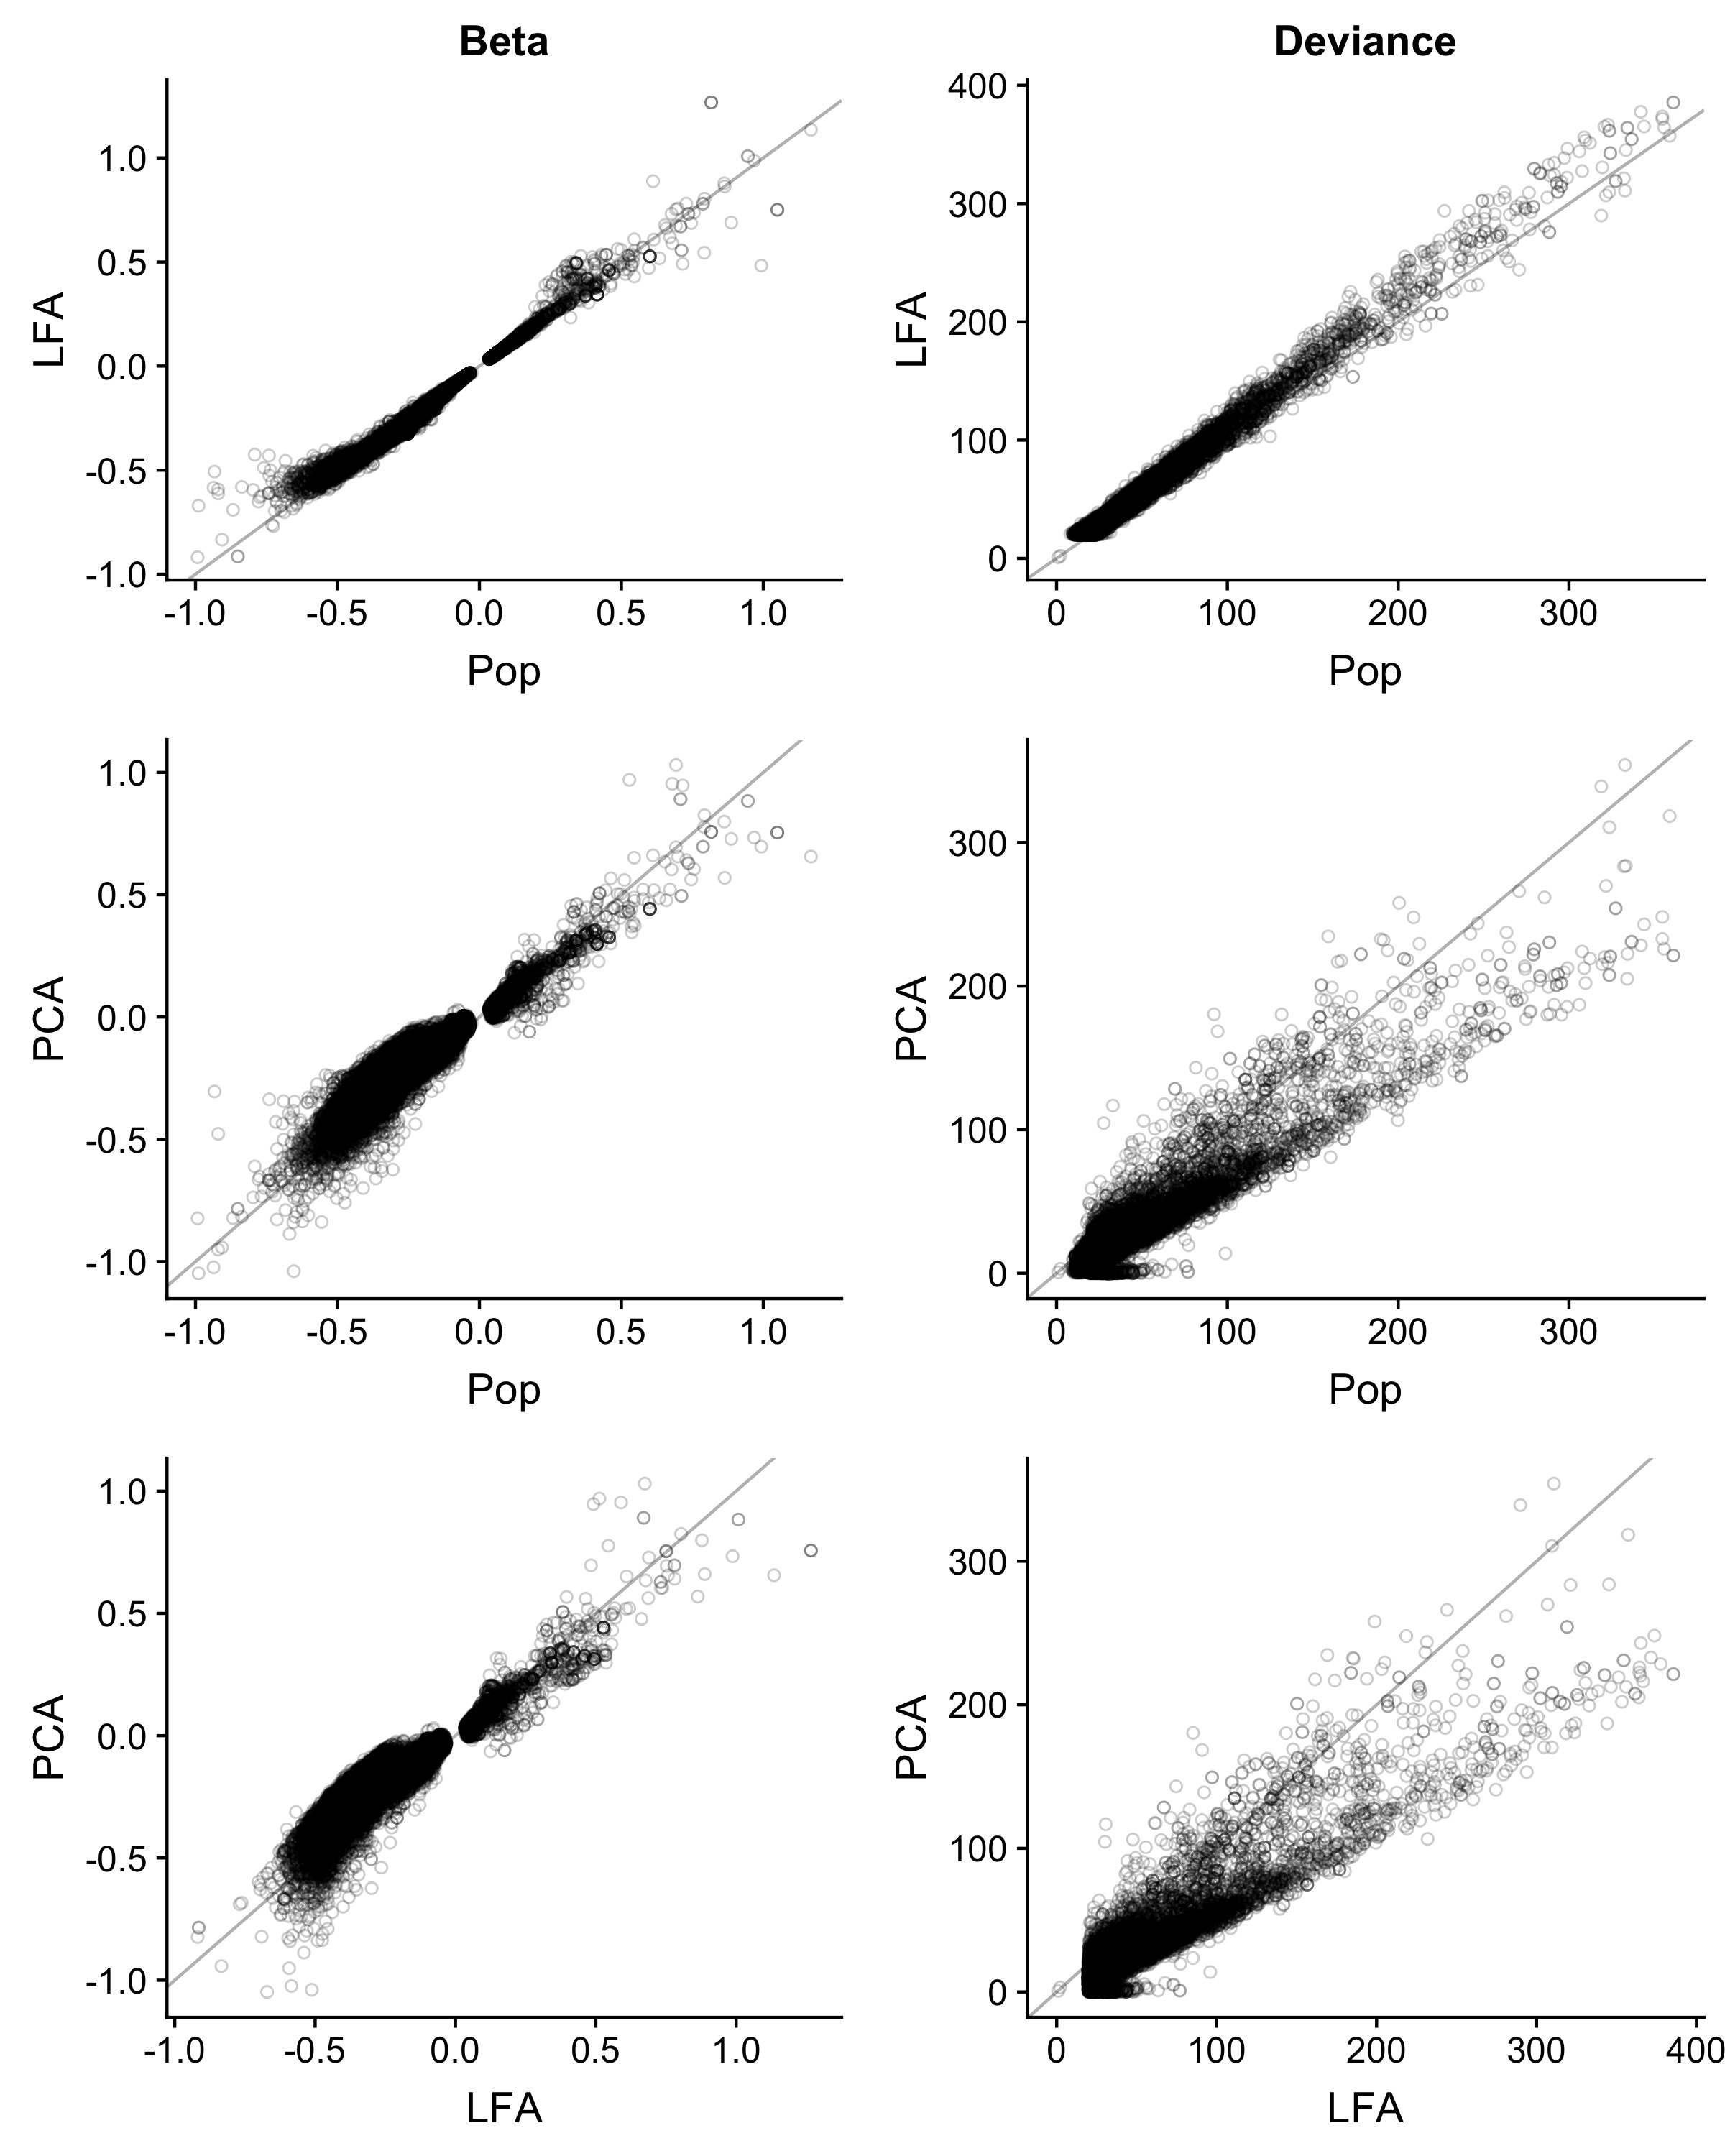
\includegraphics[width=15cm,keepaspectratio]{./Figures/fits_Significant_Positions_CompareModels.jpg}
\caption{Comparison of three logistic regression models for testing association to $Q$.
These methods model each genotype as a logistic function using principal components (PC), Population membership (Pop) or LFA as an offset.
In these plots we are comparing the deviance from the null model in the 24,390 variants identified using the LFA model.}  
\label{CompareModel}
\end{figure}

\renewcommand{\thefigure}{S\arabic{figure}}
\setcounter{figure}{0}   	

\begin{figure} \centering
    \begin{subfigure}[b]{\linewidth}
        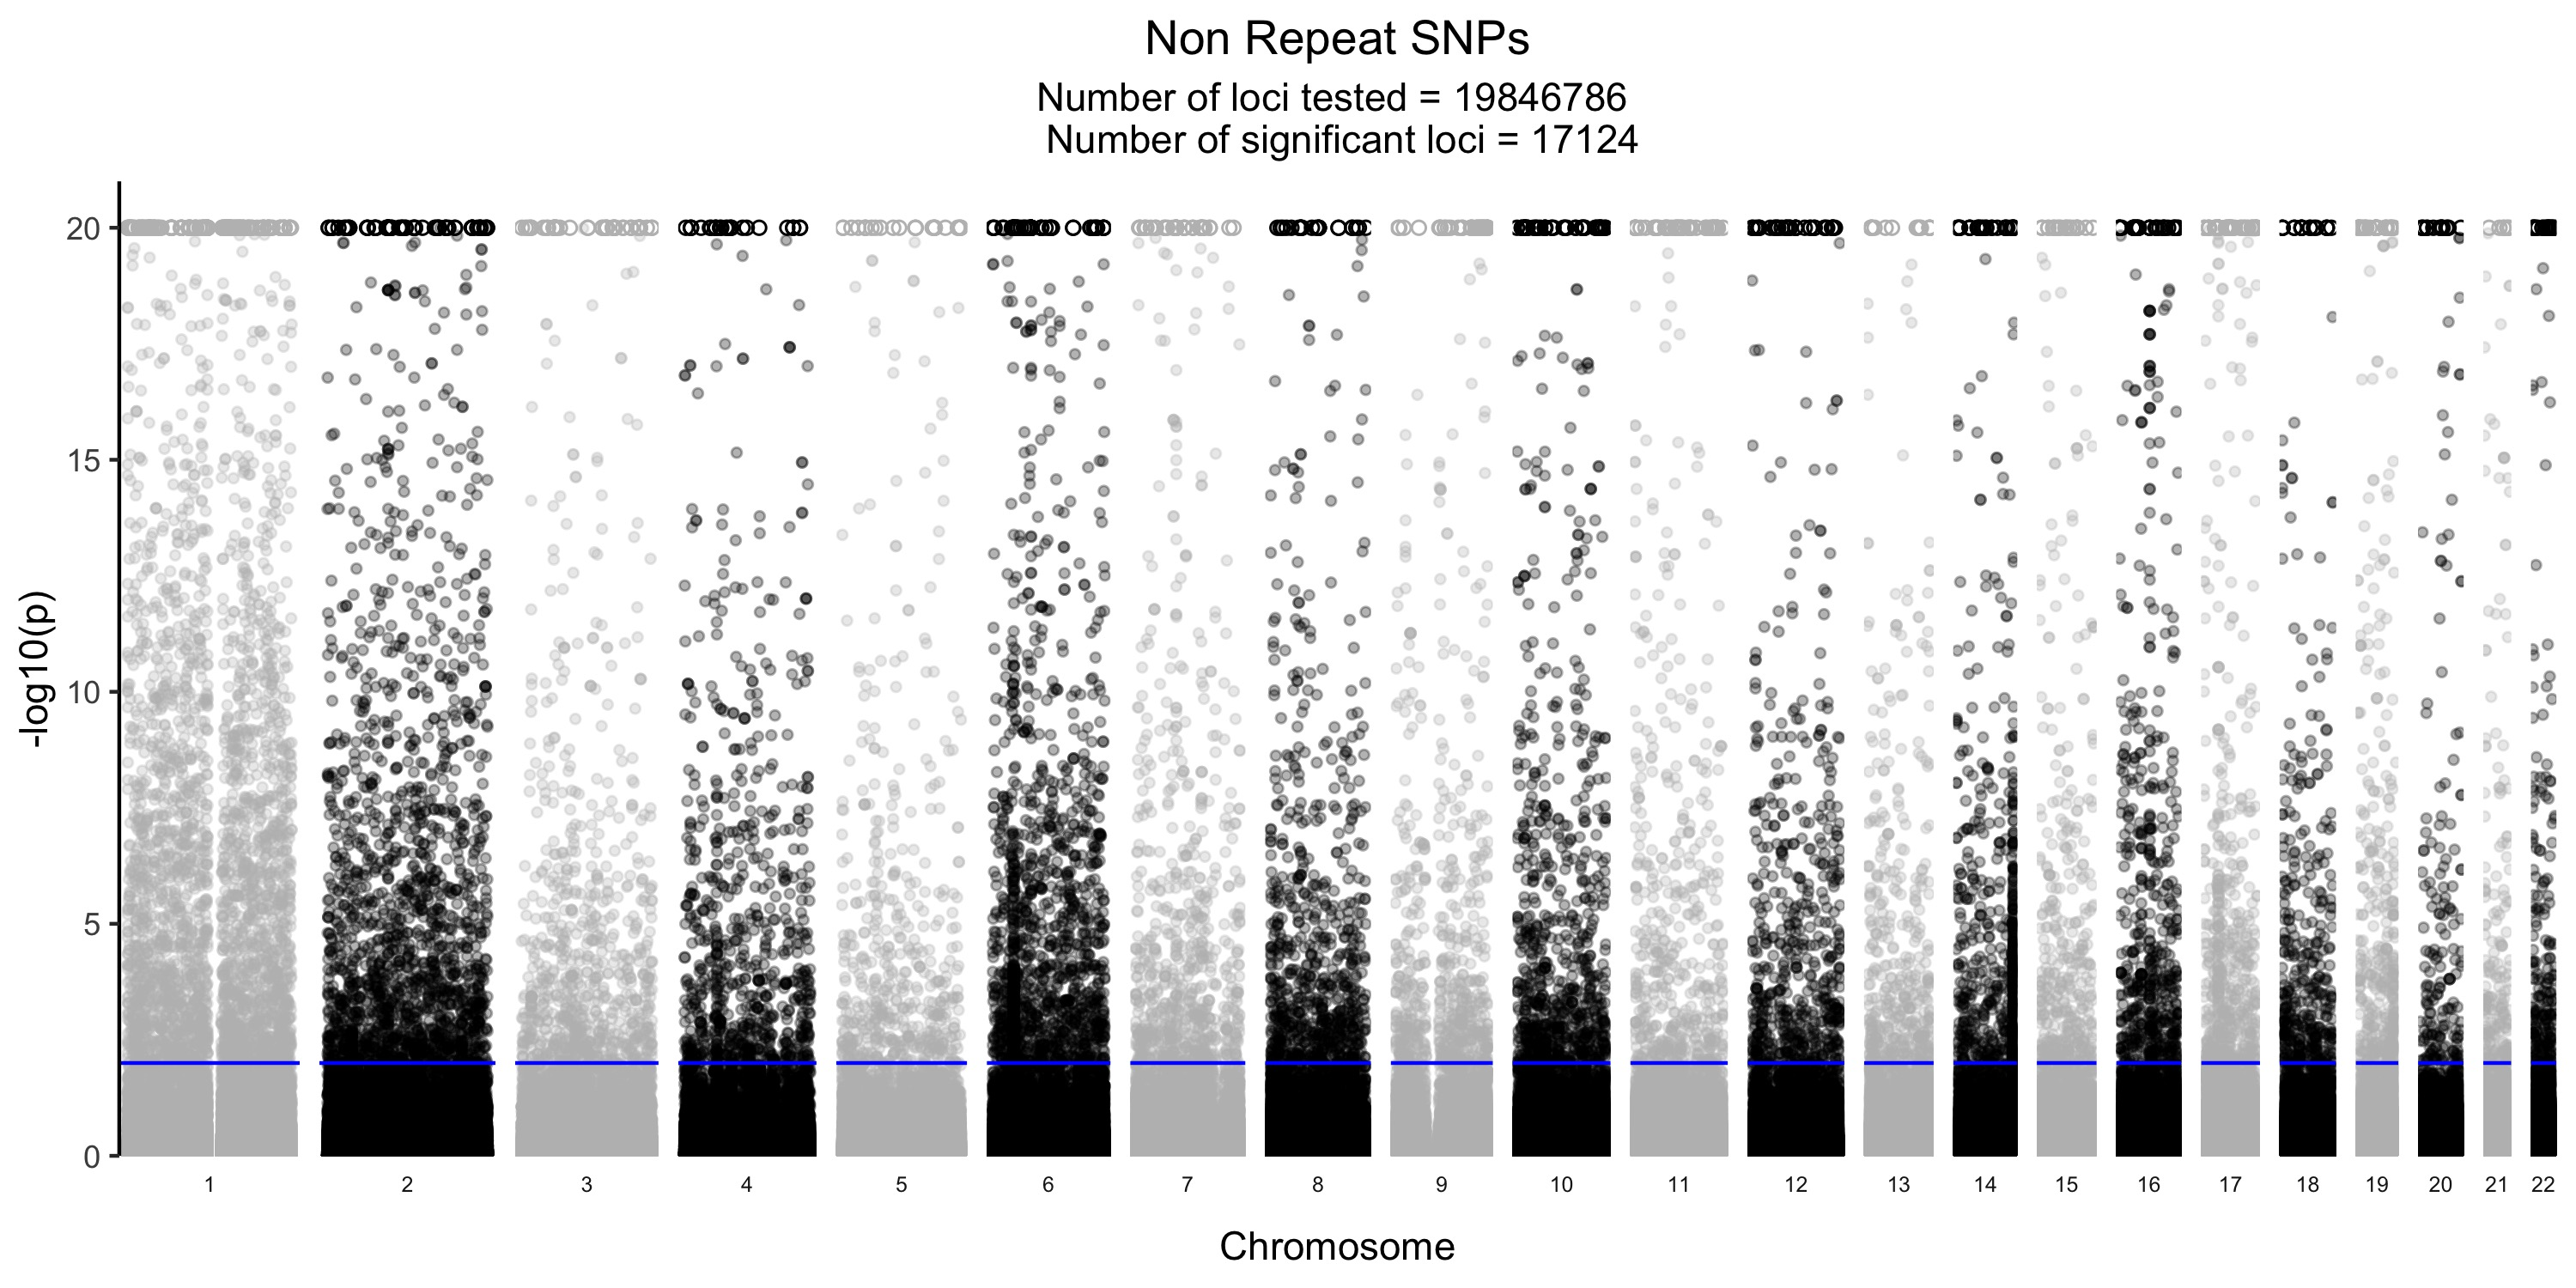
\includegraphics[width=\hsize]{./Figures/ManhattanPlot_NonRepeatSNPs.jpg}
        \label{fig:a}
    \end{subfigure} %

    \begin{subfigure}[b]{\linewidth}
    	\center    
        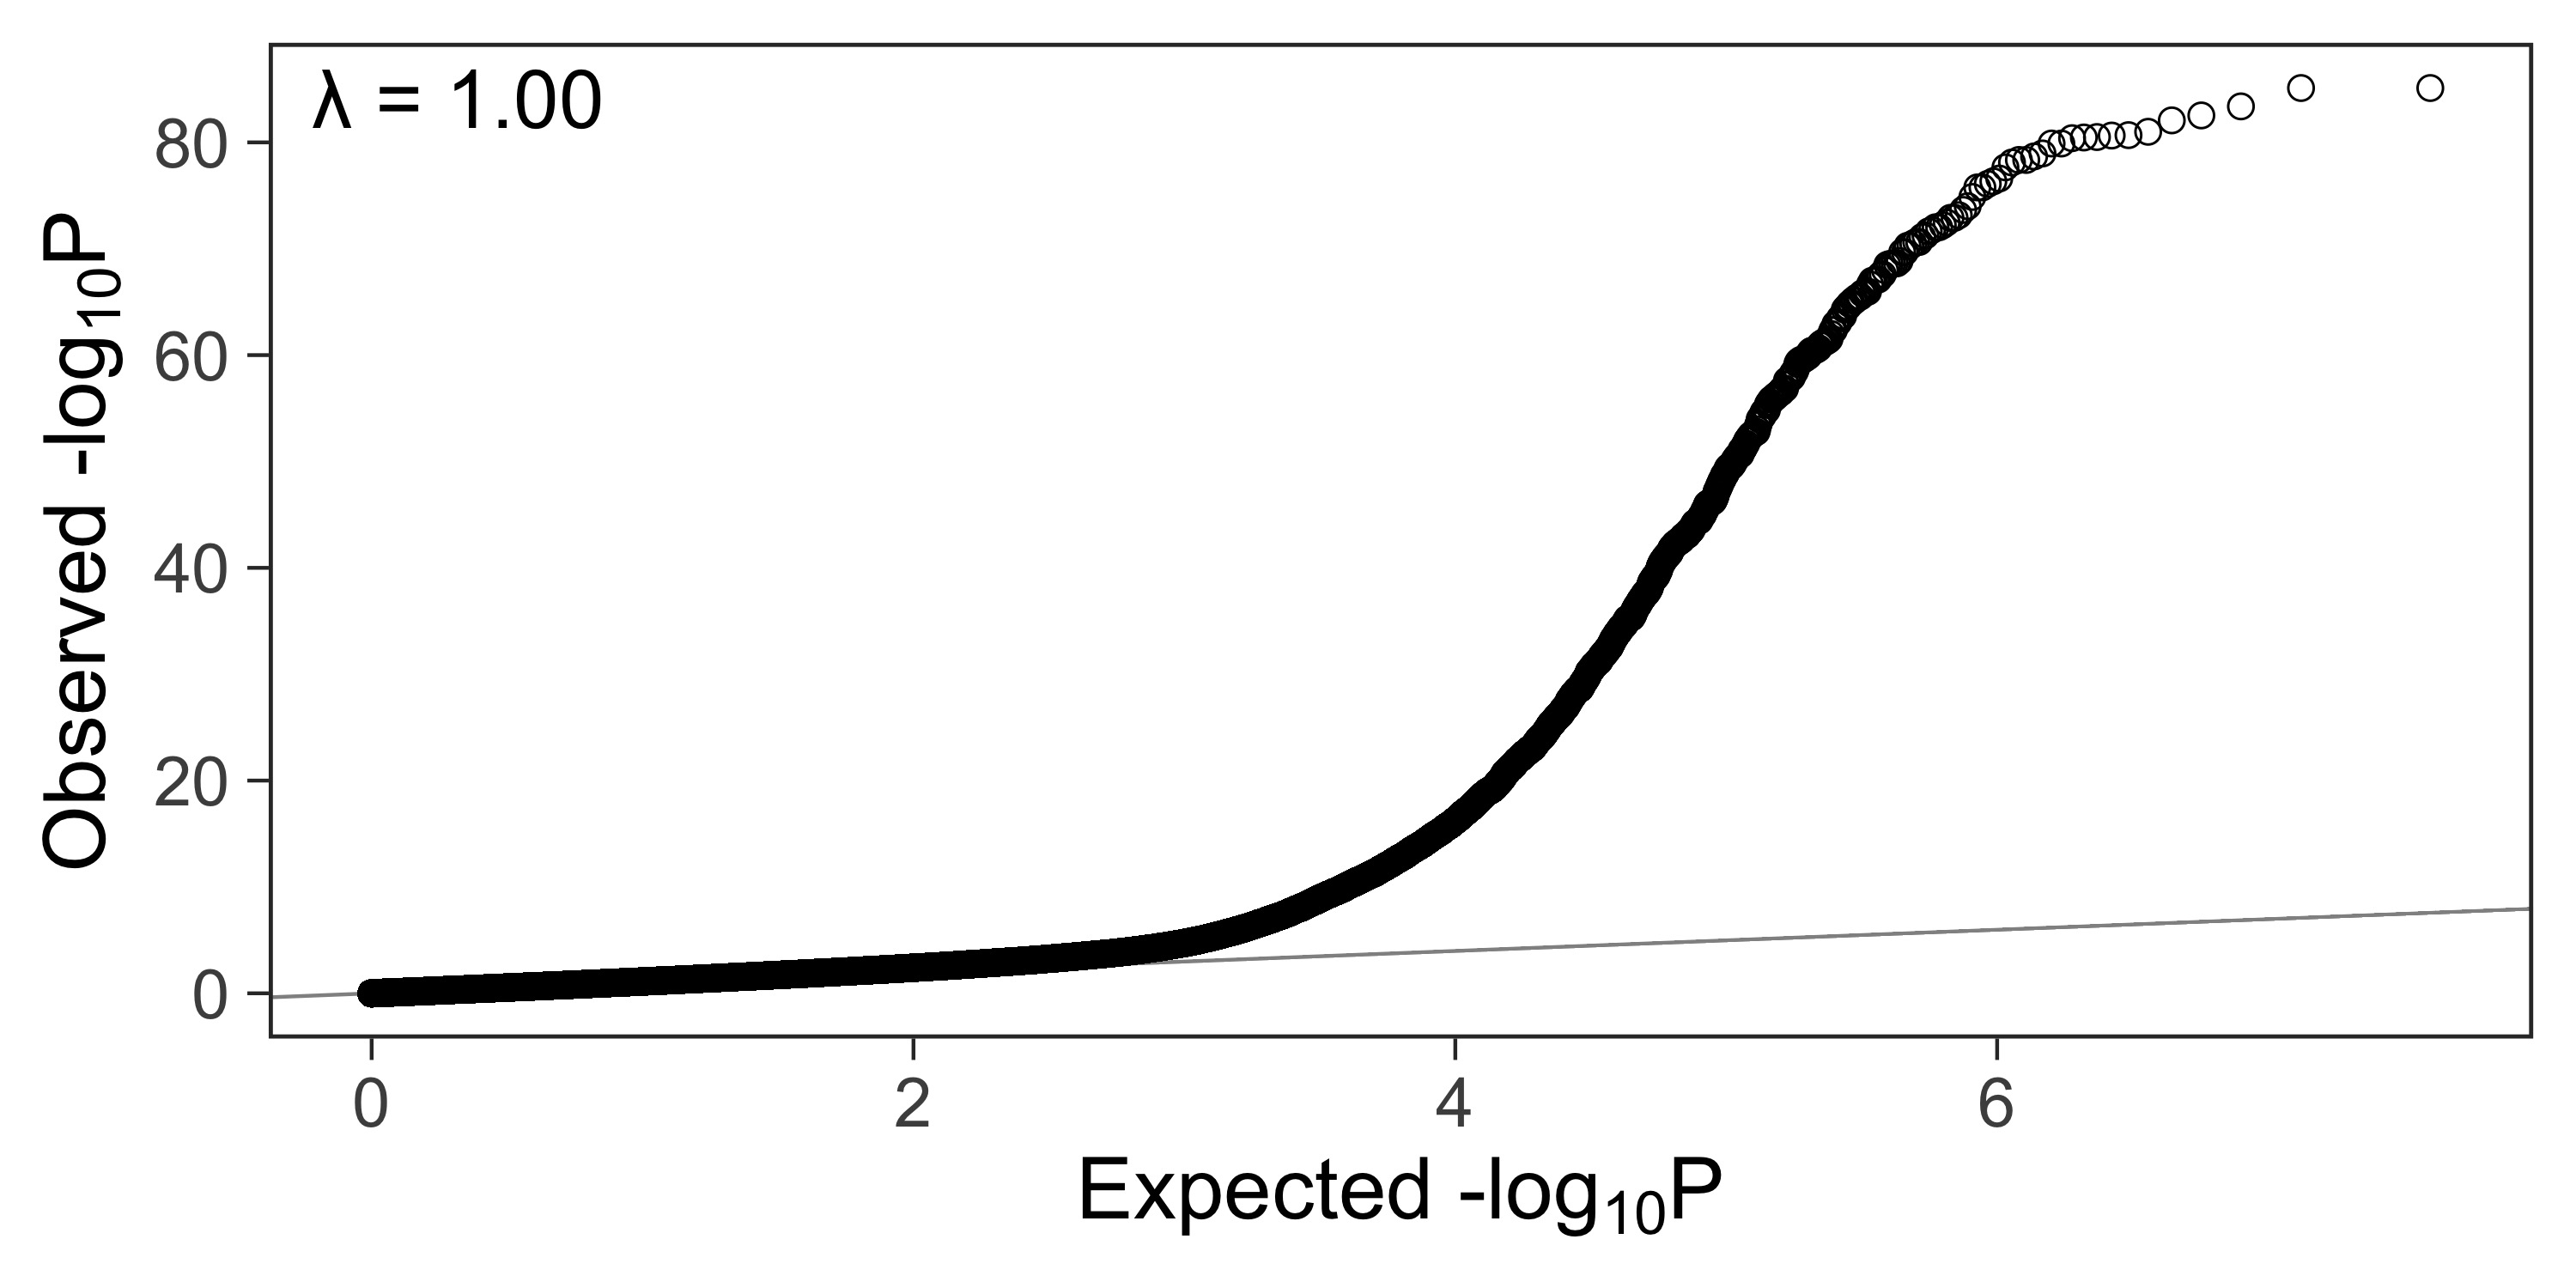
\includegraphics[width=\hsize]{./Figures/QQPlot_NonRepeatSNPs.jpg}
        \label{fig:b}    
    \end{subfigure} 
    \caption{\textbf{A} Manhattan plot of the -log10 p values for the reverse GWAS logistic regression analysis for SNPs in non repetitive regions. There are 15,018 SNPs that reach p values greater than $ p < 0.01$ after performing a two-stage Benjamini and Hochberg FDR adjustment.  The circles ( o ) are variants that reached values greater than 20, for clarity we implemented hard ceiling at 20. 
  \textbf{B} QQ plot of the unadjusted p values for the reverse GWAS logistic regression analysis for SNPs in non repetitive regions.}
  \label{NRS_Manhattan}
  \end{figure}

\begin{figure} \centering
    \begin{subfigure}[b]{\linewidth}
        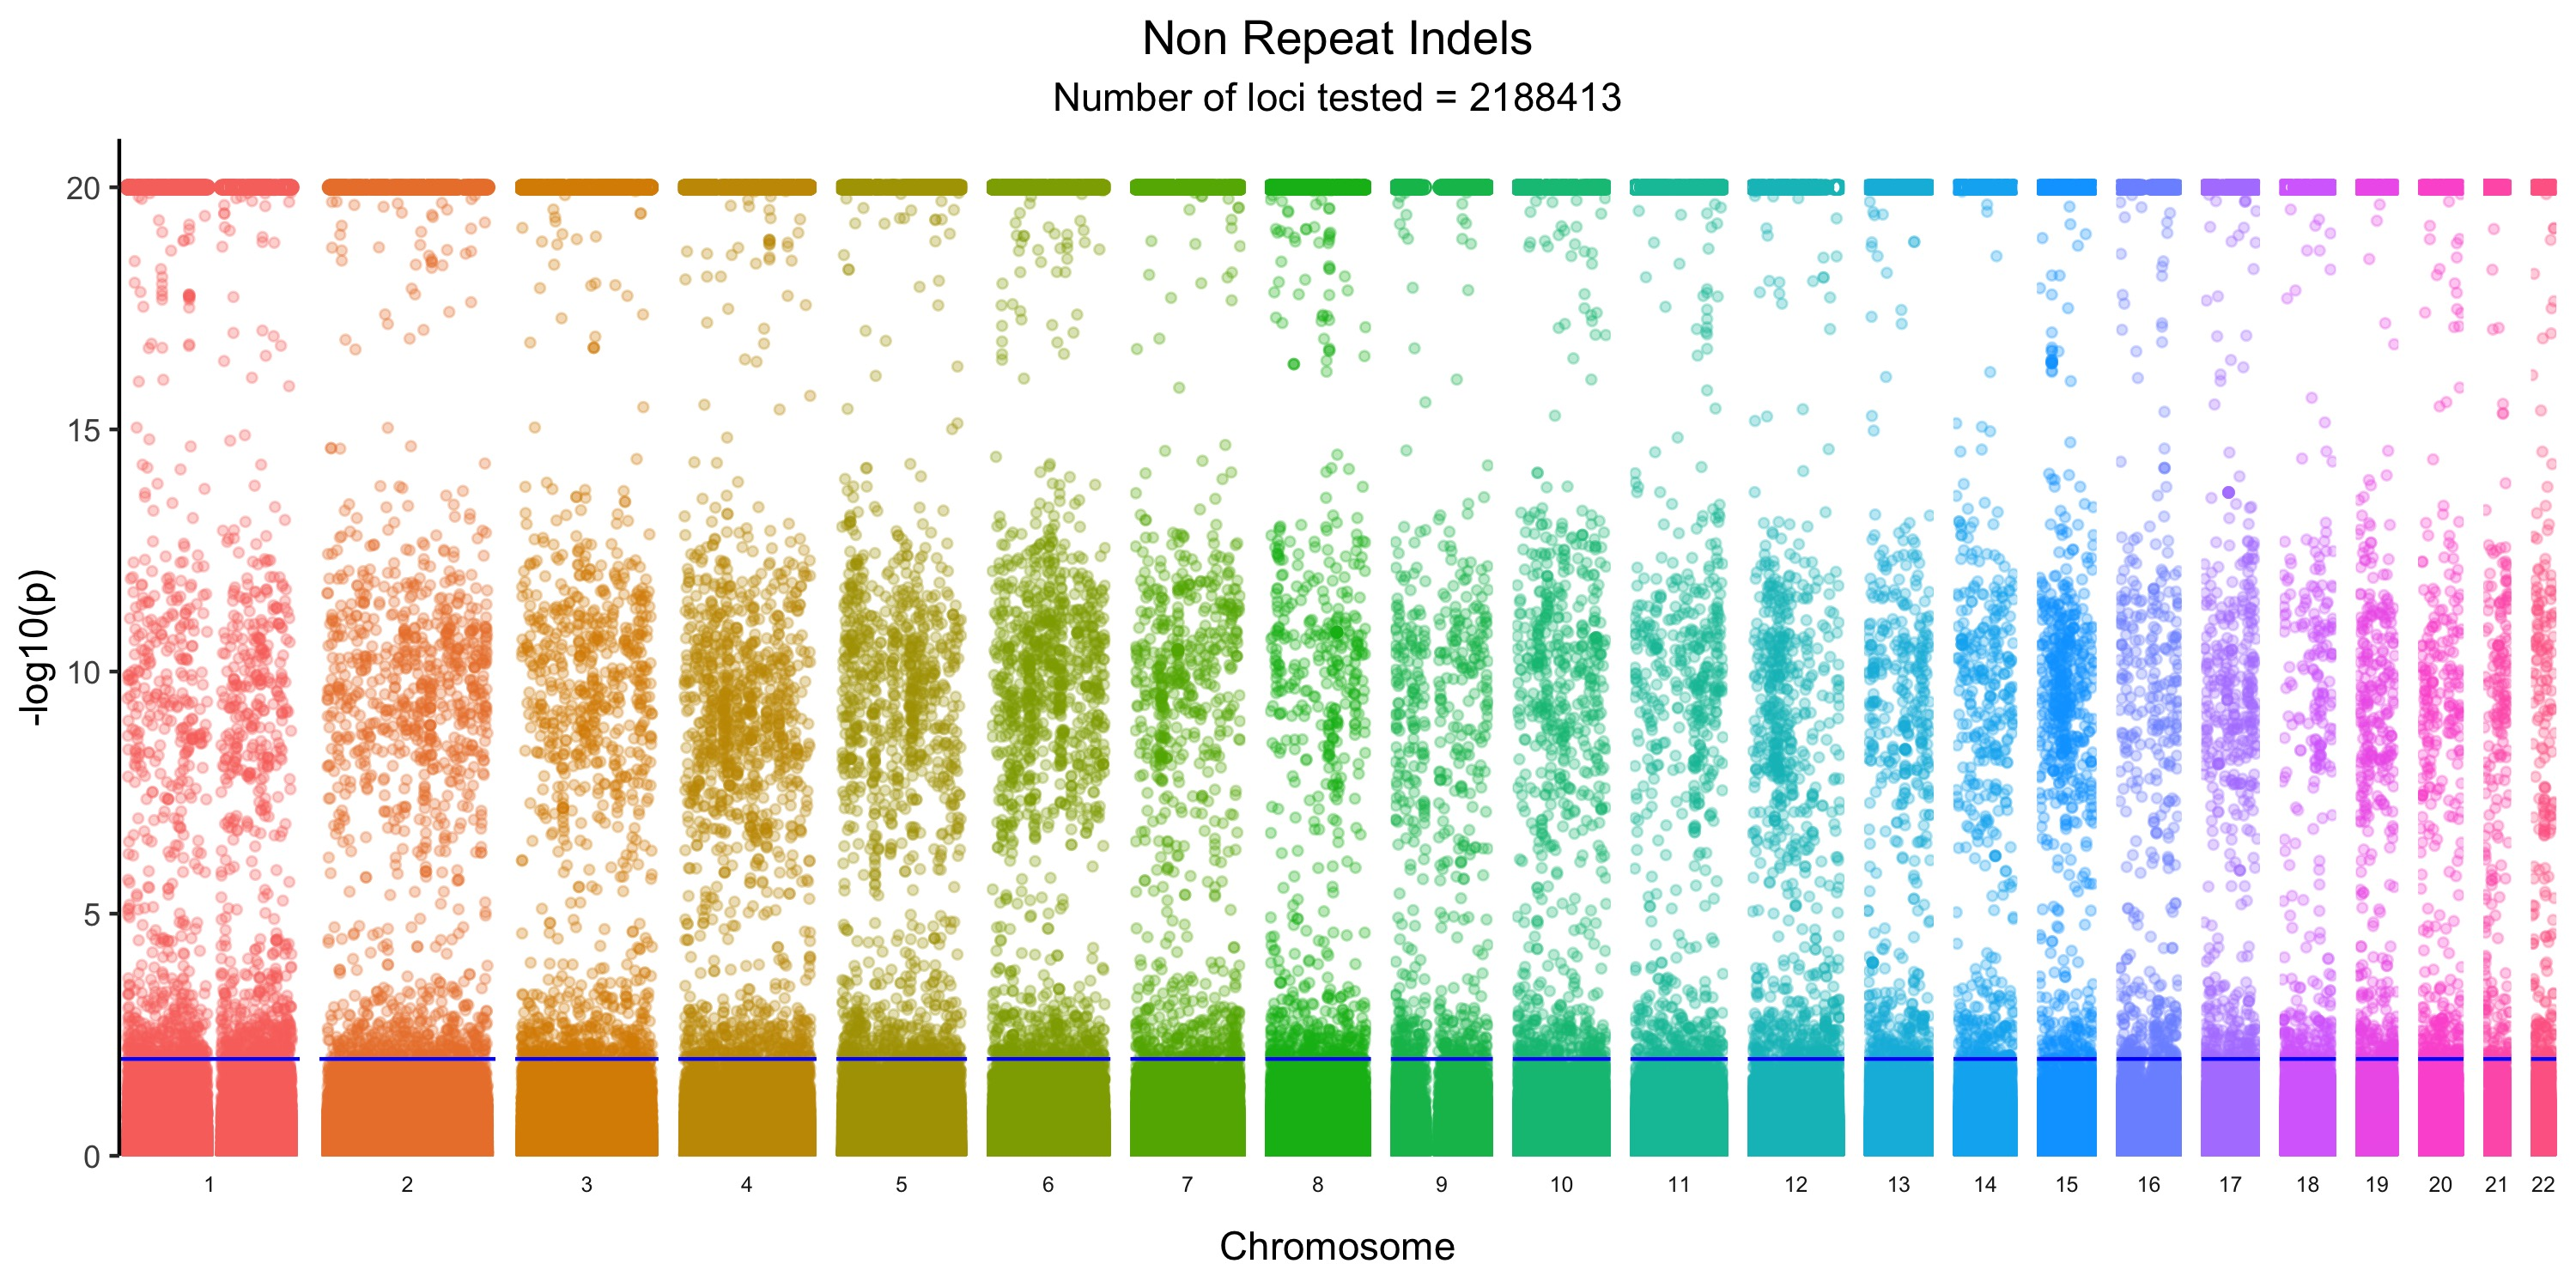
\includegraphics[width=\hsize]{./Figures/ManhattanPlot_NonRepeatIndels.jpg}
        \label{fig:a}
    \end{subfigure} %

    \begin{subfigure}[b]{\linewidth}
    	\center    
        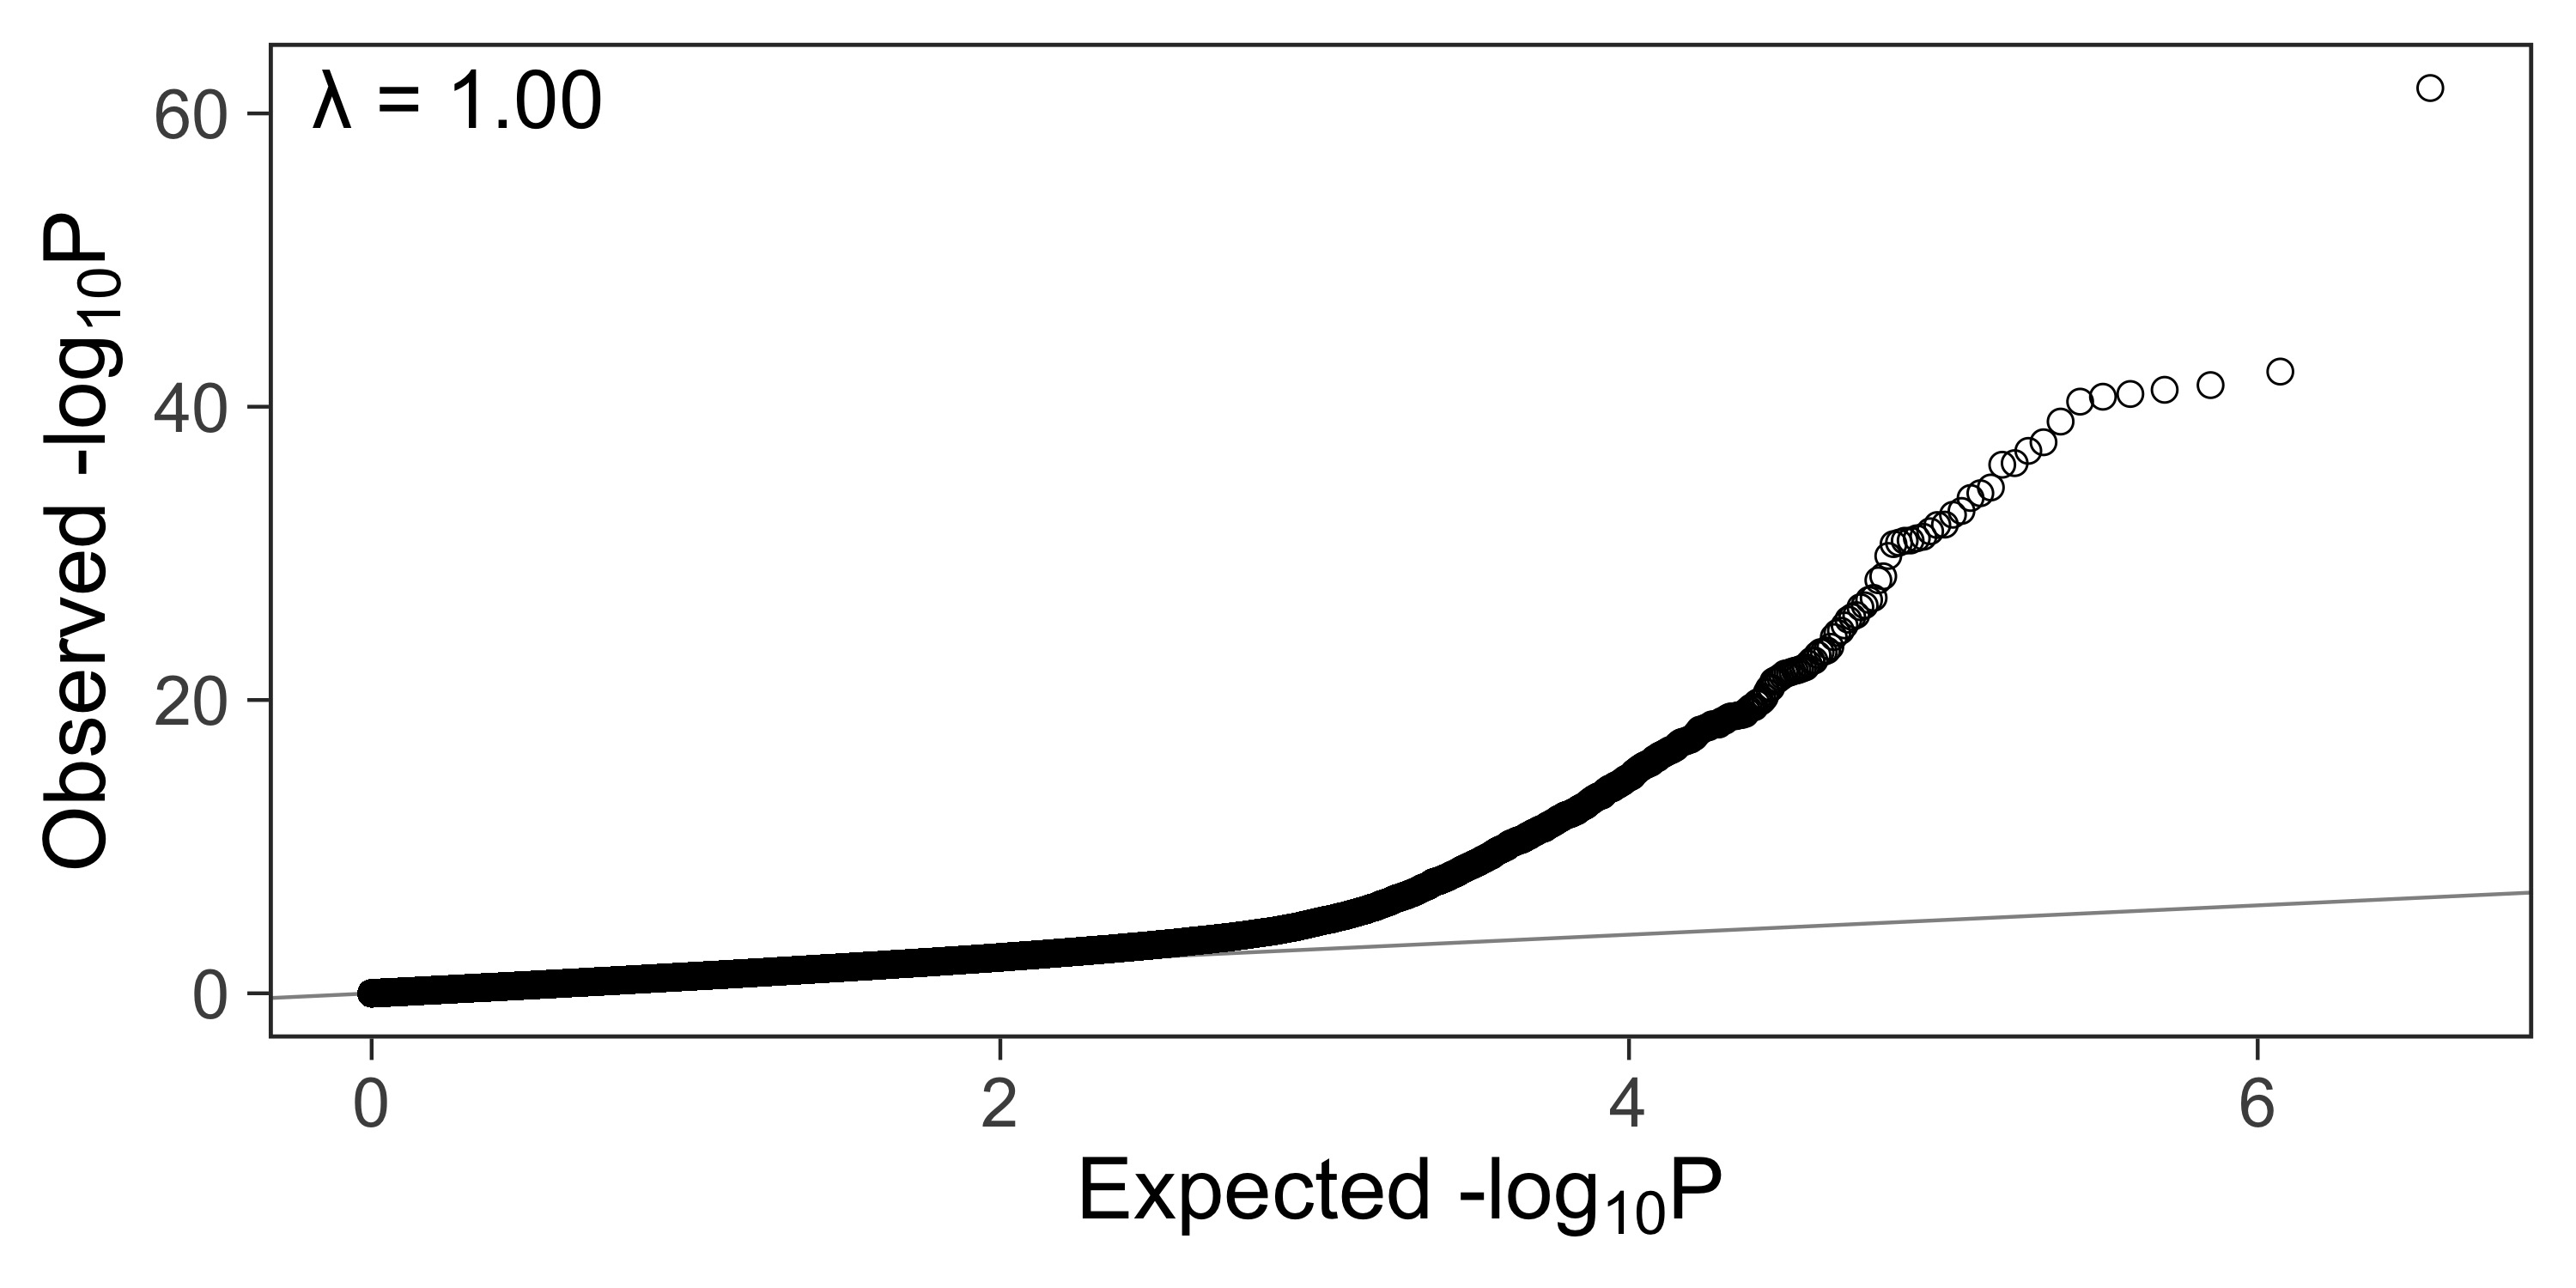
\includegraphics[width=\hsize]{./Figures/QQPlot_NonRepeatIndels.jpg}
        \label{fig:b}    
    \end{subfigure} 
    \caption{\textbf{A} Manhattan plot of the -log10 p values for the reverse GWAS logistic regression analysis for INDELs in non repetitive regions. There are 2,121 INDELs that reach p values greater than $ p < 0.01$ after performing a two-stage Benjamini and Hochberg FDR adjustment.  The circles ( o ) are variants that reached values greater than 20, for clarity we implemented hard ceiling at 20. 
  \textbf{B} QQ plot of the unadjusted p values for the reverse GWAS logistic regression analysis for INDELs in non repetitive regions.}
  \label{NRI_Manhattan}
  \end{figure}

\begin{figure} \centering
    \begin{subfigure}[b]{\linewidth}
        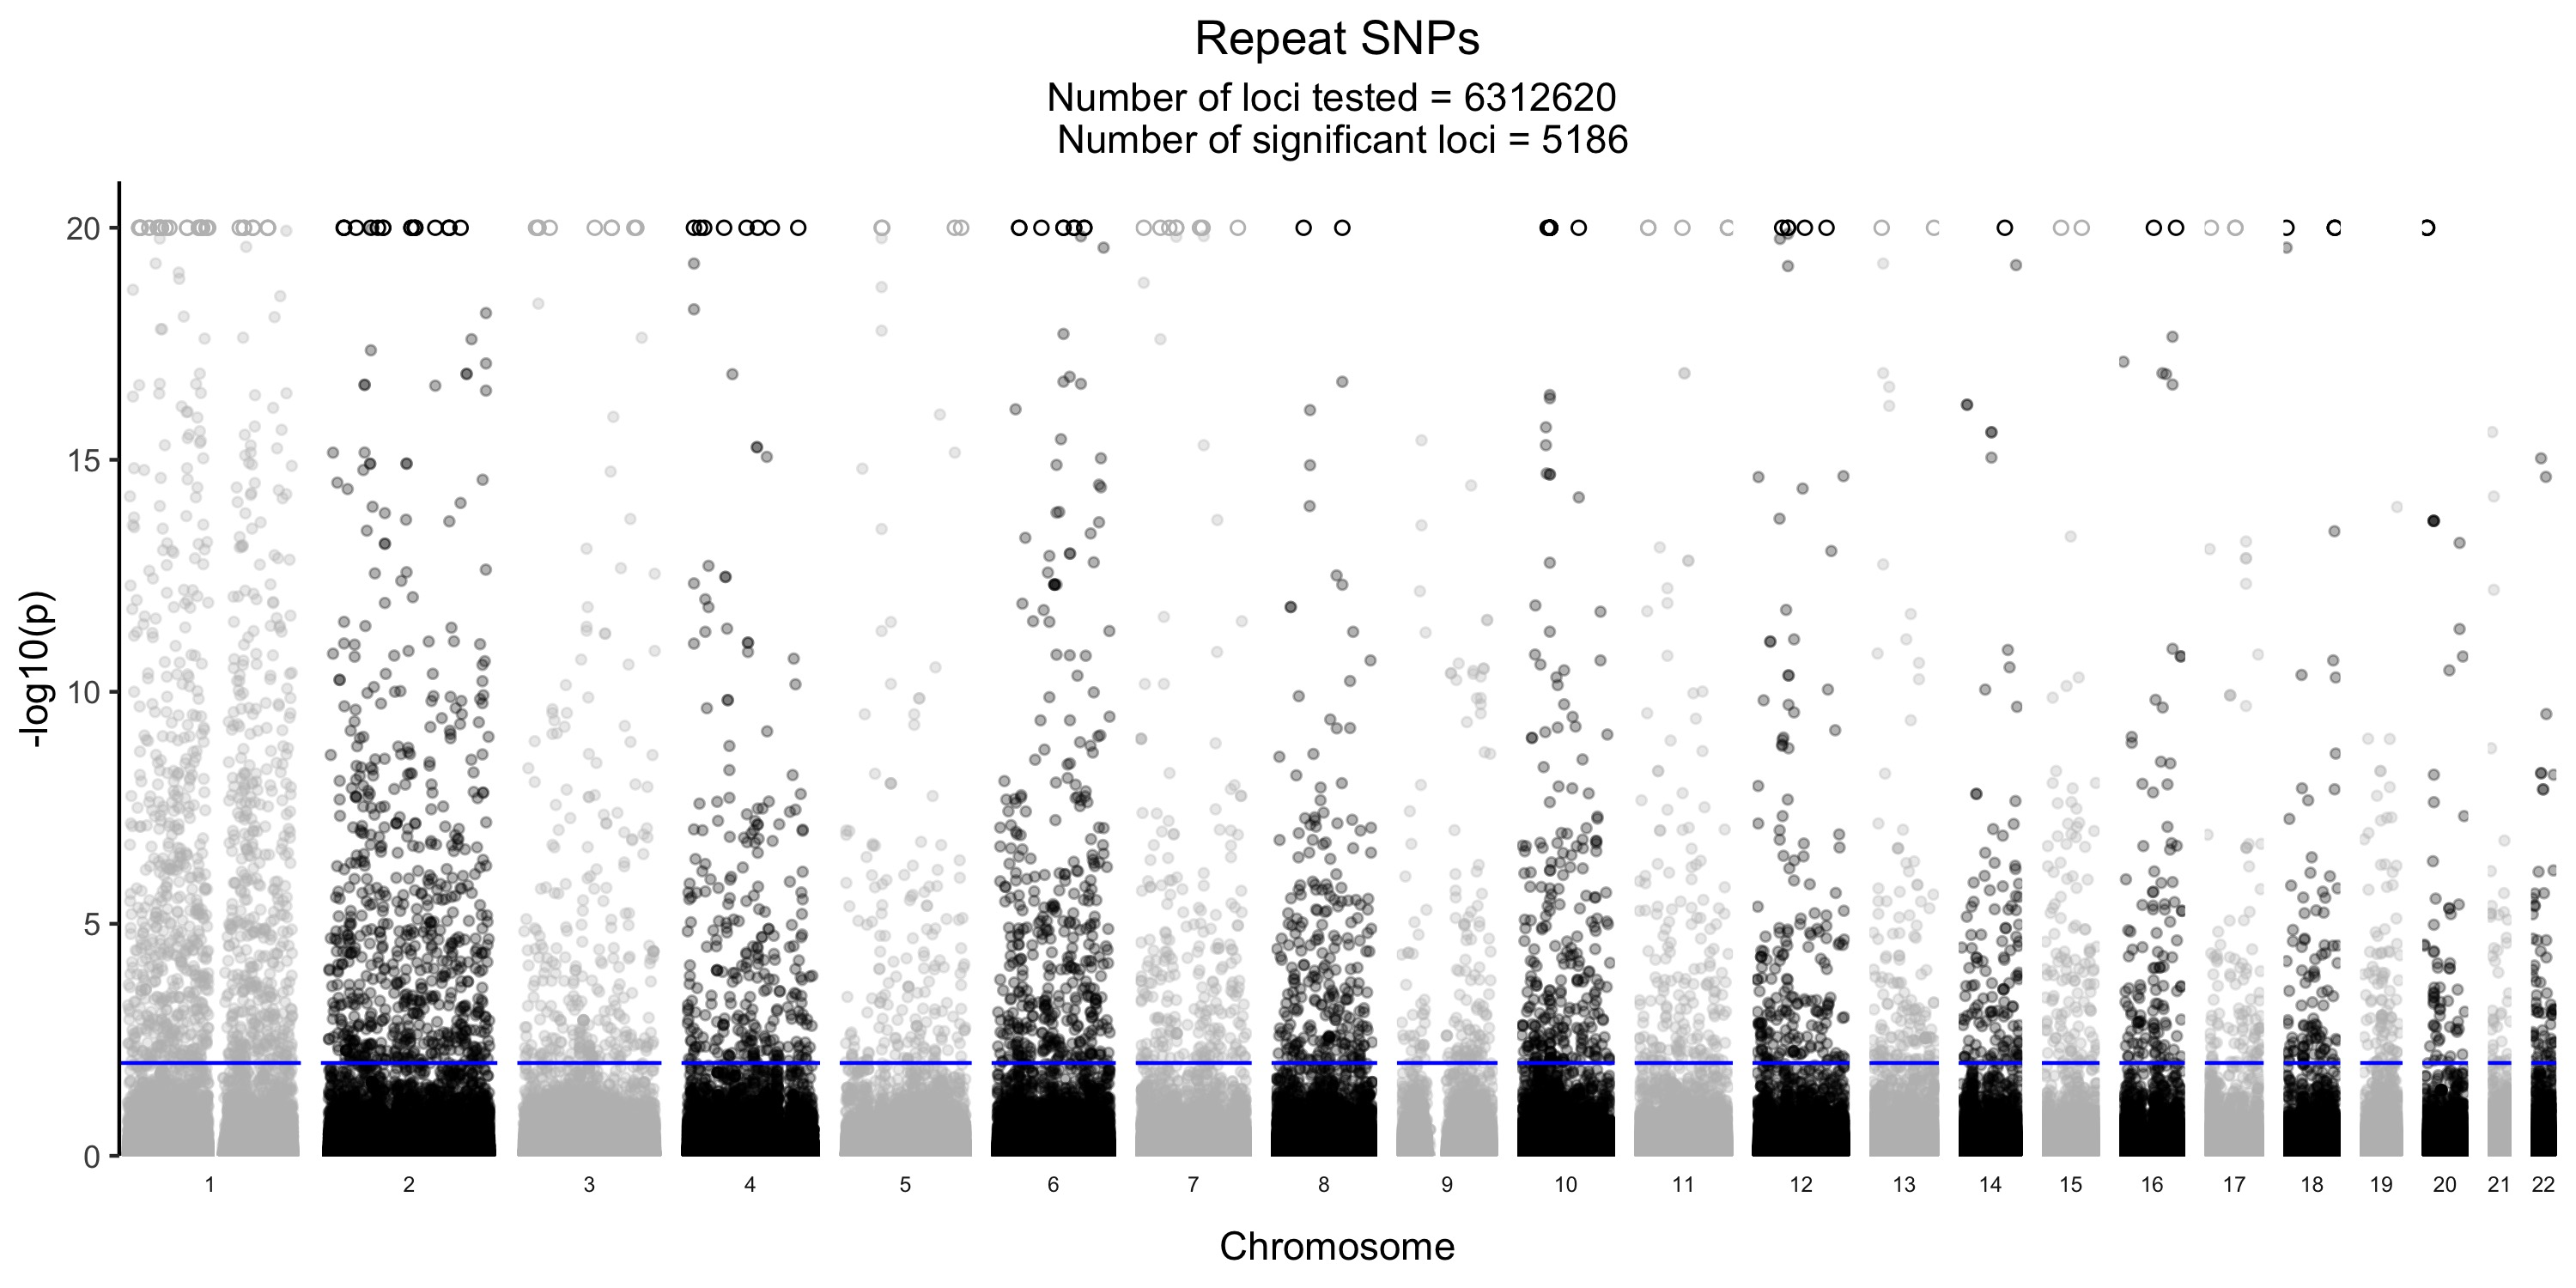
\includegraphics[width=\hsize]{./Figures/ManhattanPlot_RepeatSNPs.jpg}
        \label{fig:a}
    \end{subfigure} %

    \begin{subfigure}[b]{\linewidth}
    	\center    
        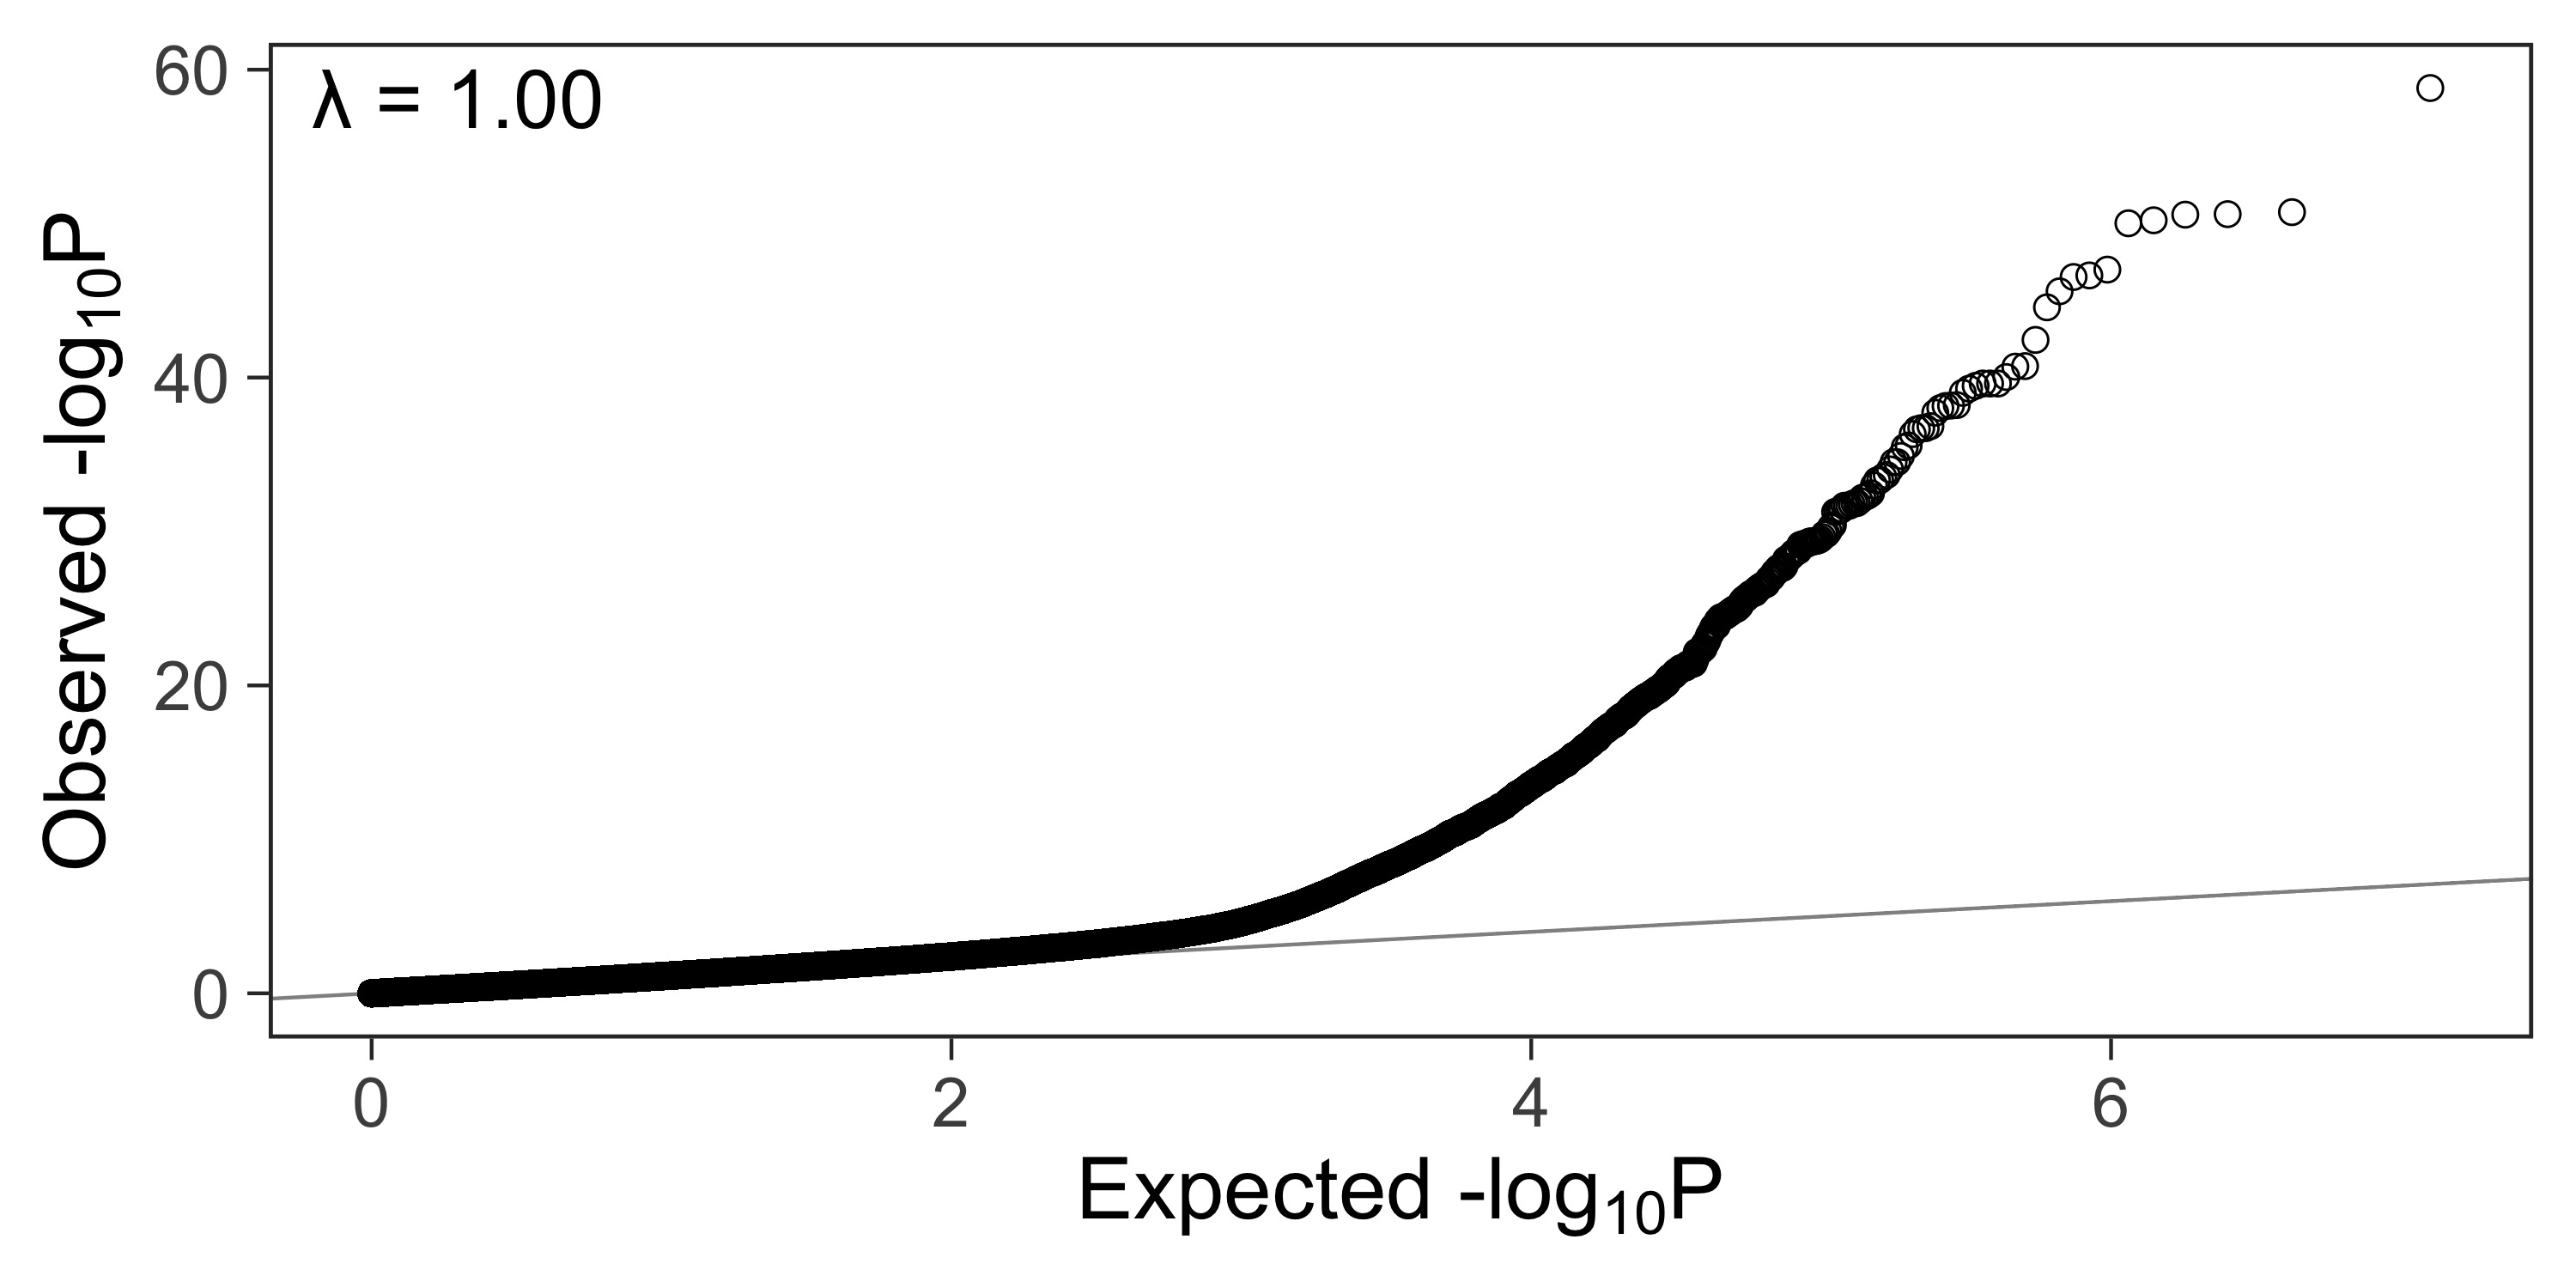
\includegraphics[width=\hsize]{./Figures/QQPlot_RepeatSNPs.jpg}
        \label{fig:b}    
    \end{subfigure} 
    \caption{\textbf{A} Manhattan plot of the -log10 p values for the reverse GWAS logistic regression analysis for SNPs in repetitive regions. There are 4,405 SNPs that reach p values greater than $ p < 0.01$ after performing a two-stage Benjamini and Hochberg FDR adjustment.  The circles ( o ) are variants that reached values greater than 20, for clarity we implemented hard ceiling at 20. 
  \textbf{B} QQ plot of the unadjusted p values for the reverse GWAS logistic regression analysis for SNPs in repetitive regions.}
  \label{RS_Manhattan}
  \end{figure}
  
\begin{figure} \centering
    \begin{subfigure}[b]{\linewidth}
        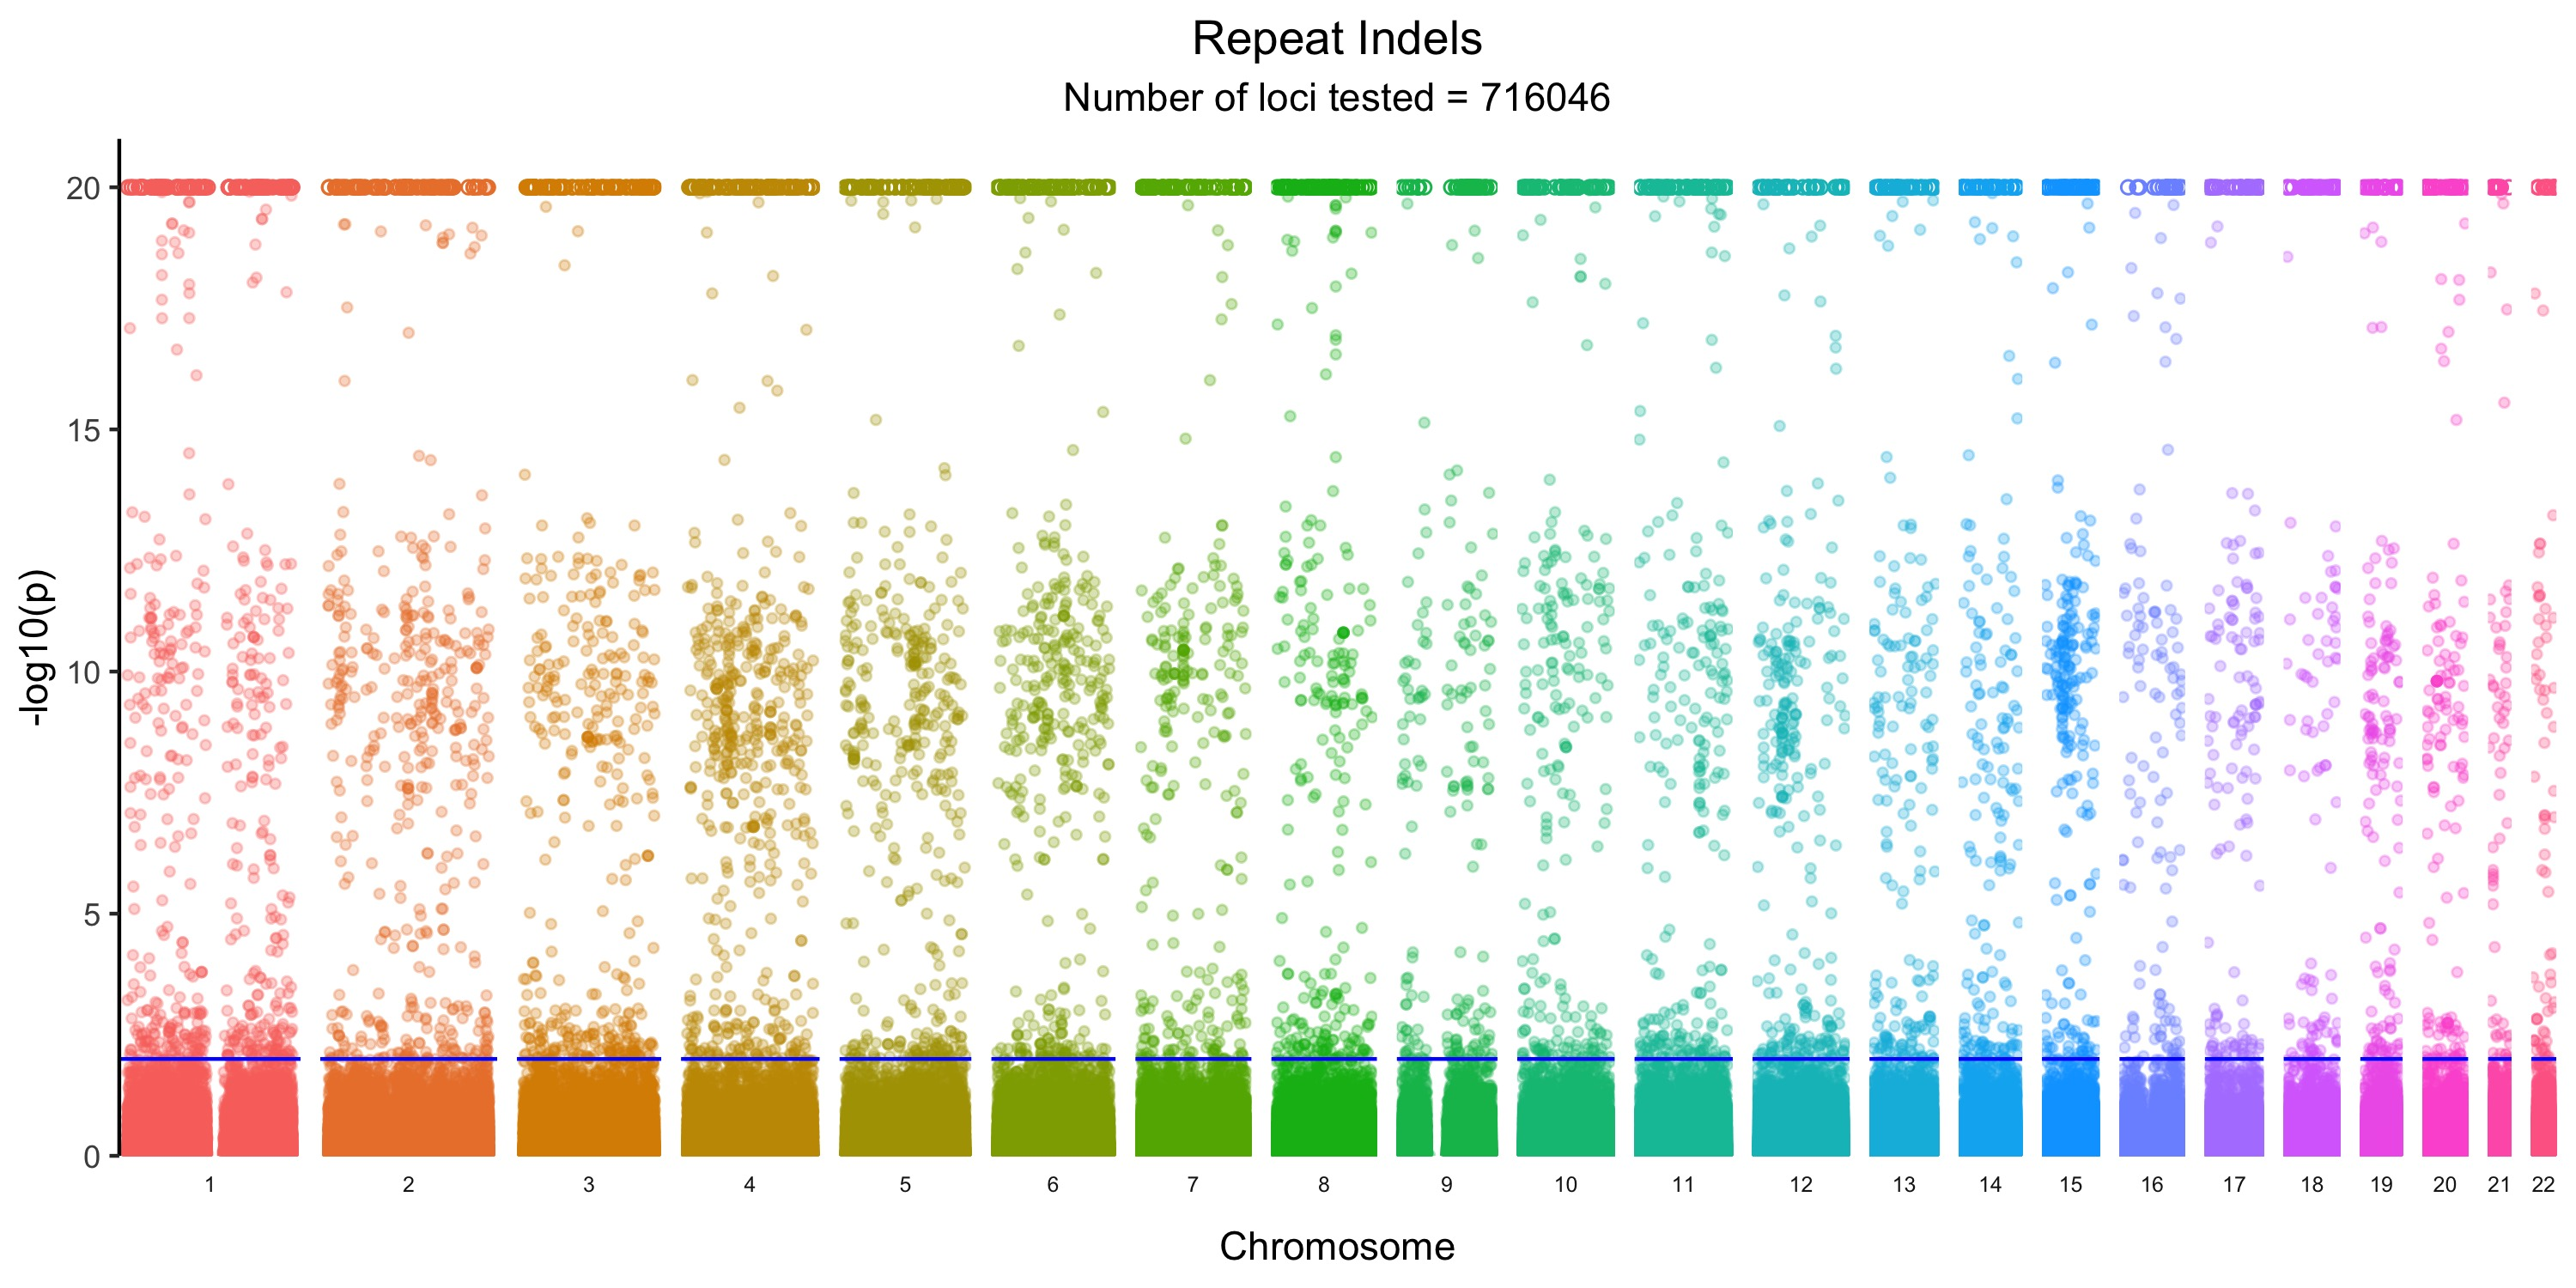
\includegraphics[width=\hsize]{./Figures/ManhattanPlot_RepeatIndels.jpg}
        \label{fig:a}
    \end{subfigure} %

    \begin{subfigure}[b]{\linewidth}
    	\center    
        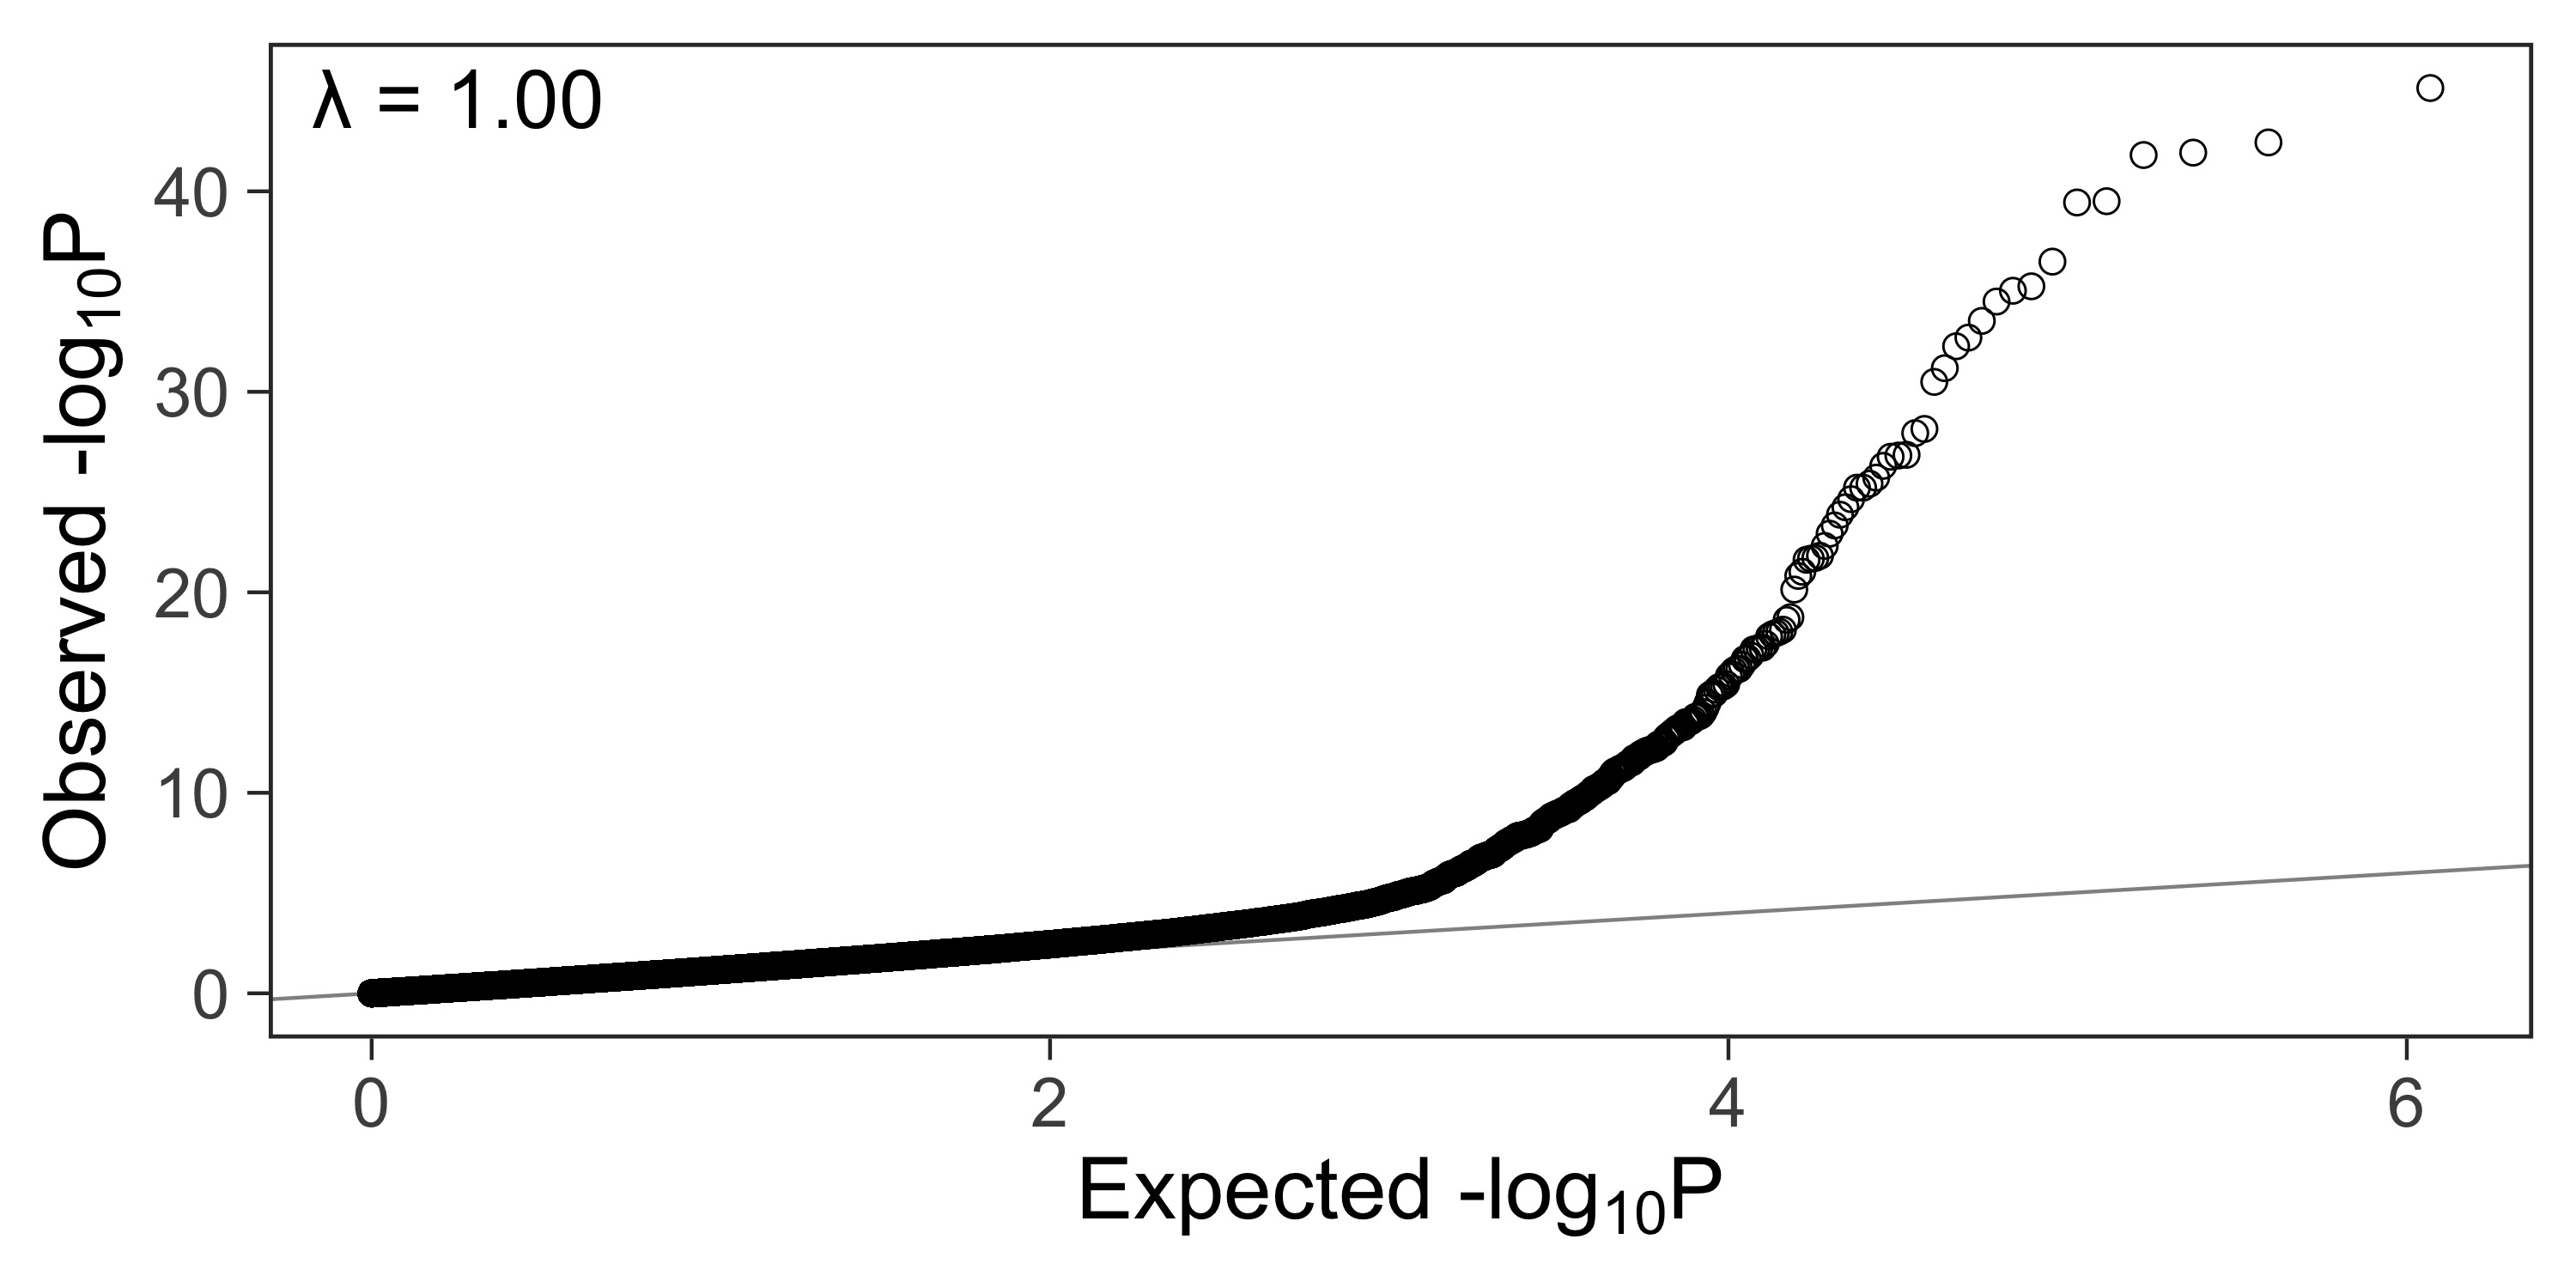
\includegraphics[width=\hsize]{./Figures/QQPlot_RepeatIndels.jpg}
        \label{fig:b}    
    \end{subfigure} 
    \caption{\textbf{A} Manhattan plot of the -log10 p values for the reverse GWAS logistic regression analysis for INDELs in repetitive regions. There are 642 INDELs that reach p values greater than $ p < 0.01$ after performing a two-stage Benjamini and Hochberg FDR adjustment.  The circles ( o ) are variants that reached values greater than 20, for clarity we implemented hard ceiling at 20. 
  \textbf{B} QQ plot of the unadjusted p values for the reverse GWAS logistic regression analysis for INDELs in repetitive regions.}
  \label{RI_Manhattan}
  \end{figure}


\begin{figure}[h]
\centering
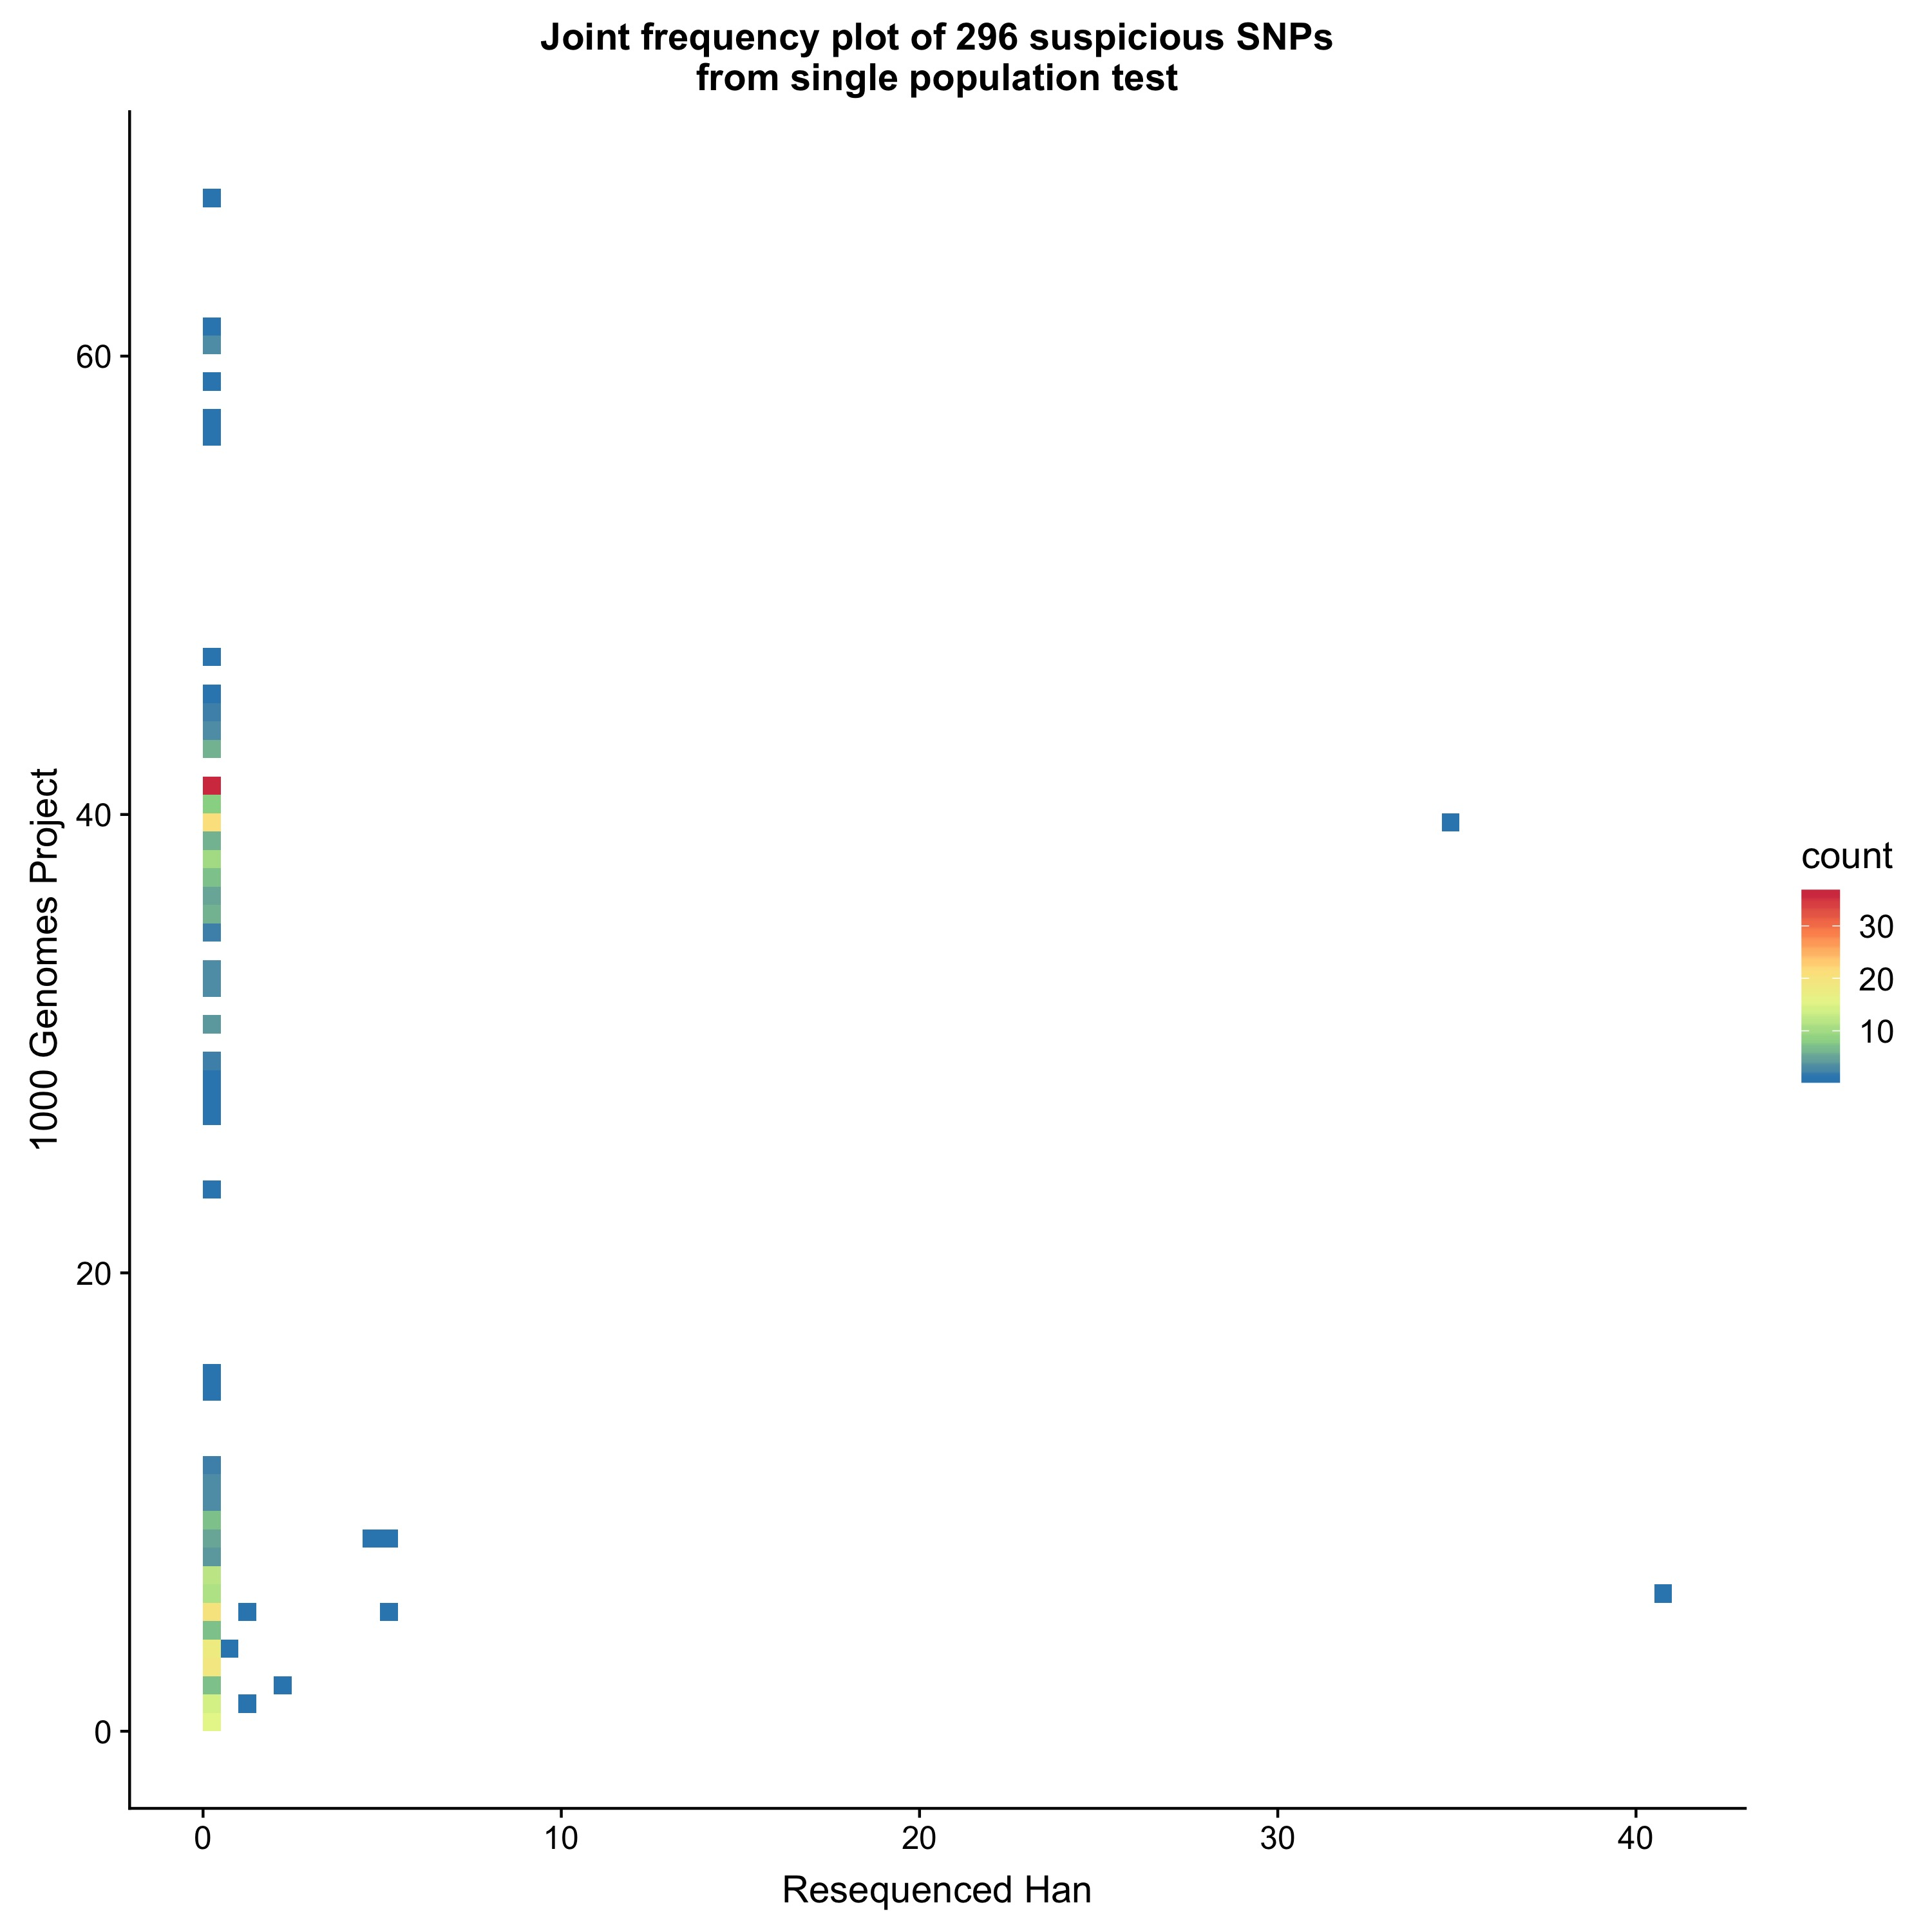
\includegraphics[width=12cm,keepaspectratio]{./Figures/Han_1kGP_SFS_singlePop.jpg}
\caption{Site frequency spectrum plot comparing the original 1kGP data to the high depth resequence data. This plot only shows significant SNPs identified in the single population tests of CHS and CHB populations. Only 9 of the 296 significant SNPs identified in the resequenced Han samples \citep{Lan2017}.
Because the resequencing did not include all the individuals from the original 1kGP dataset, we downsampled the data to match the resequenced individuals.}  
\label{90HanSFS}
\end{figure}

\begin{figure}[h]
\centering
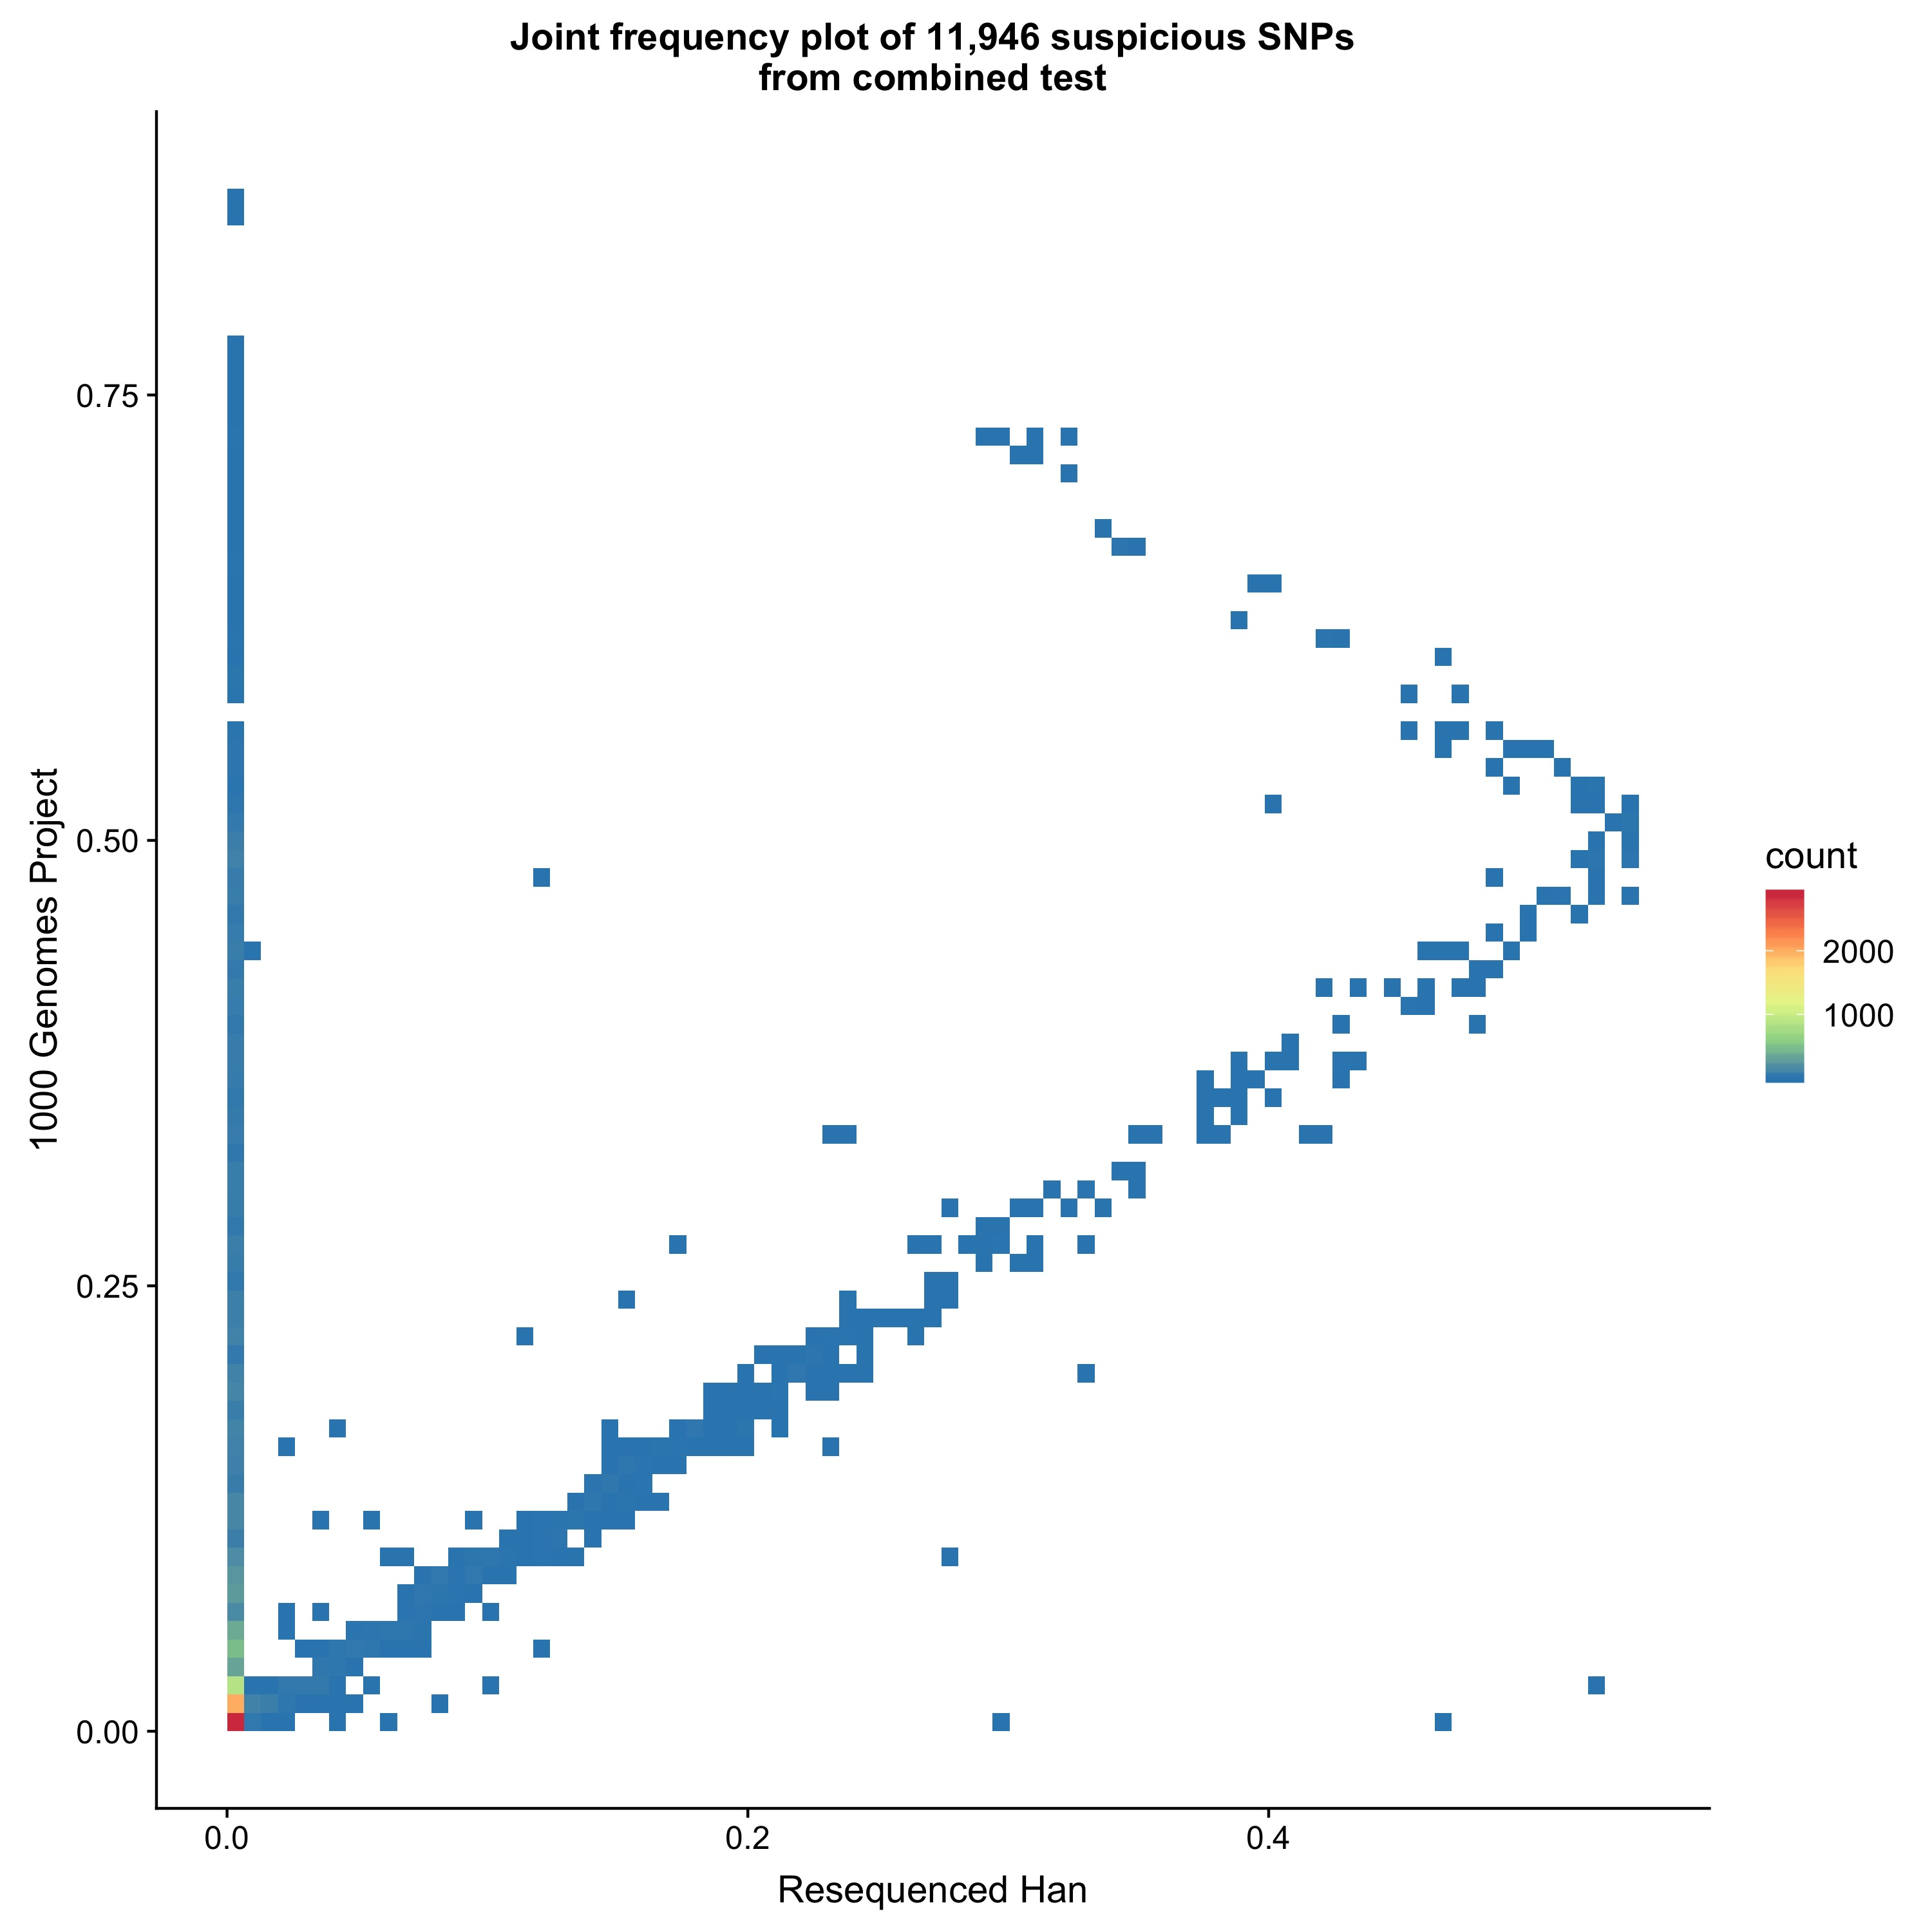
\includegraphics[width=12cm,keepaspectratio]{./Figures/Han_1kGP_SFS_FullModel.jpg}
\caption{Site frequency spectrum plot comparing the original 1kGP data to the high depth resequenced data. 
This plot shows  12,086 significant variants identified in the reverse GWAS model including all populations.
 Only 1,637 of the variants are present in the high depth resequenced individuals.}  
\label{90HanSFS_full}
\end{figure}

\begin{figure}[h]
\centering
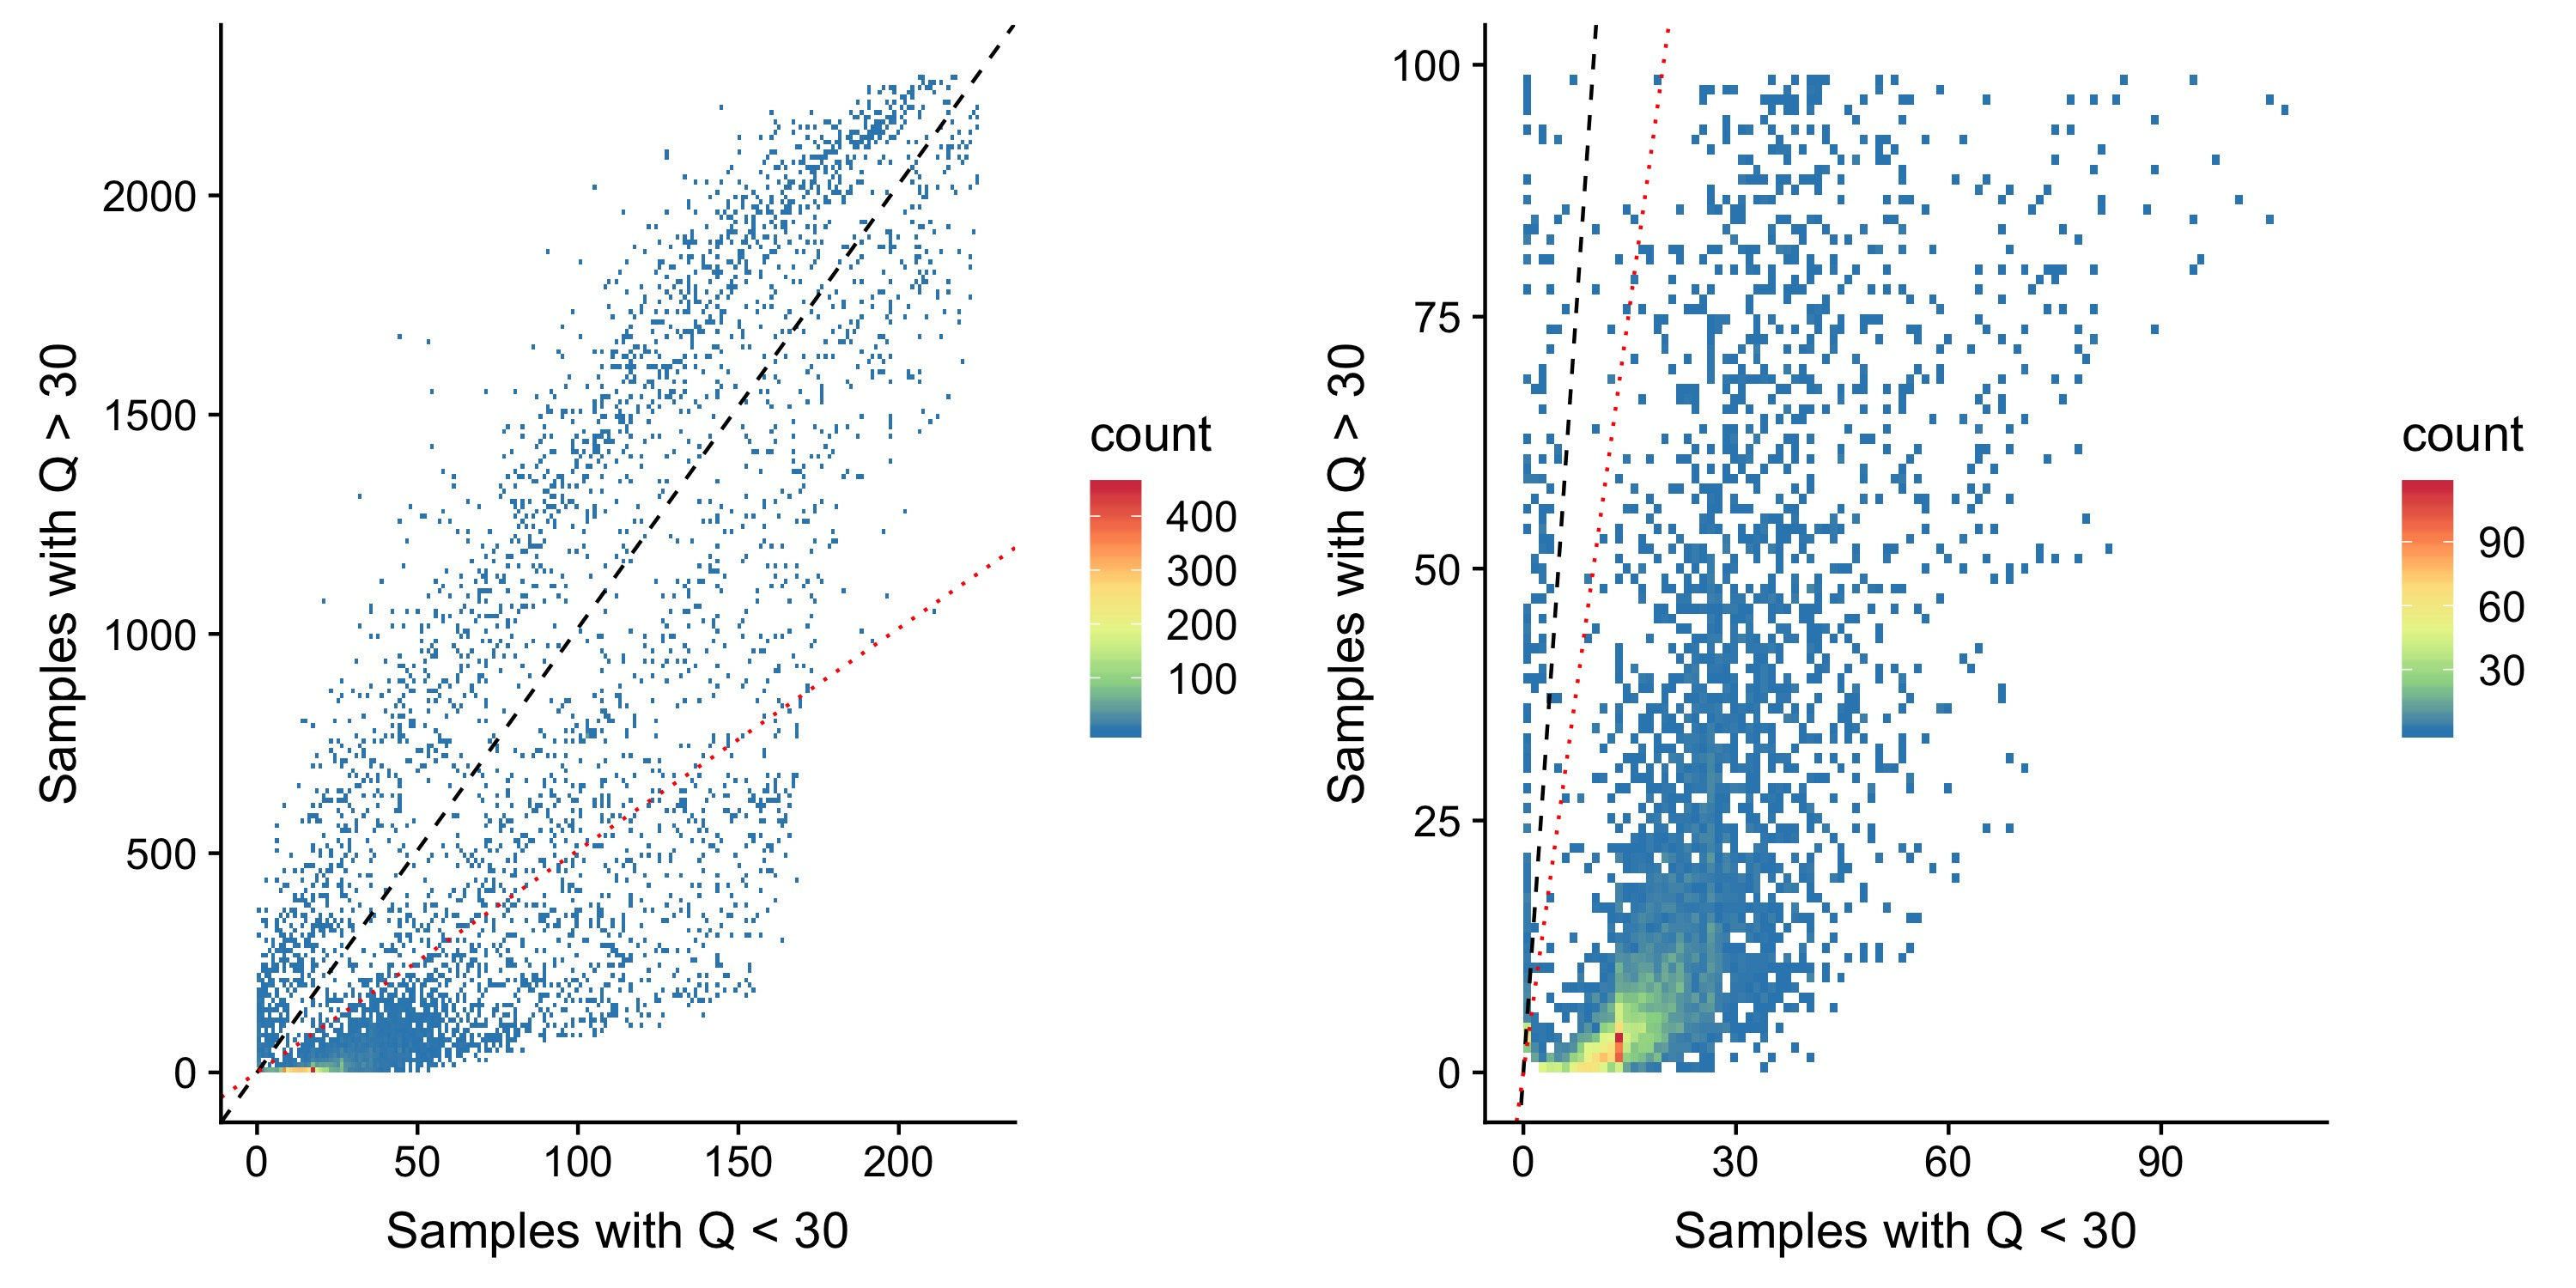
\includegraphics[width=15cm,keepaspectratio]{./Figures/OverUnder30.jpg}
\caption{Site frequency spectrum plot comparing the frequency of suspicious variants for individuals with $Q$ scores above and below 30. The black dashed lines indicates equal allele frequencies while the red dotted line for variants twice as frequent in individuals with $Q$ scores below 30.}  
\label{90HanSFS_full}
\end{figure}

\begin{figure}[h]
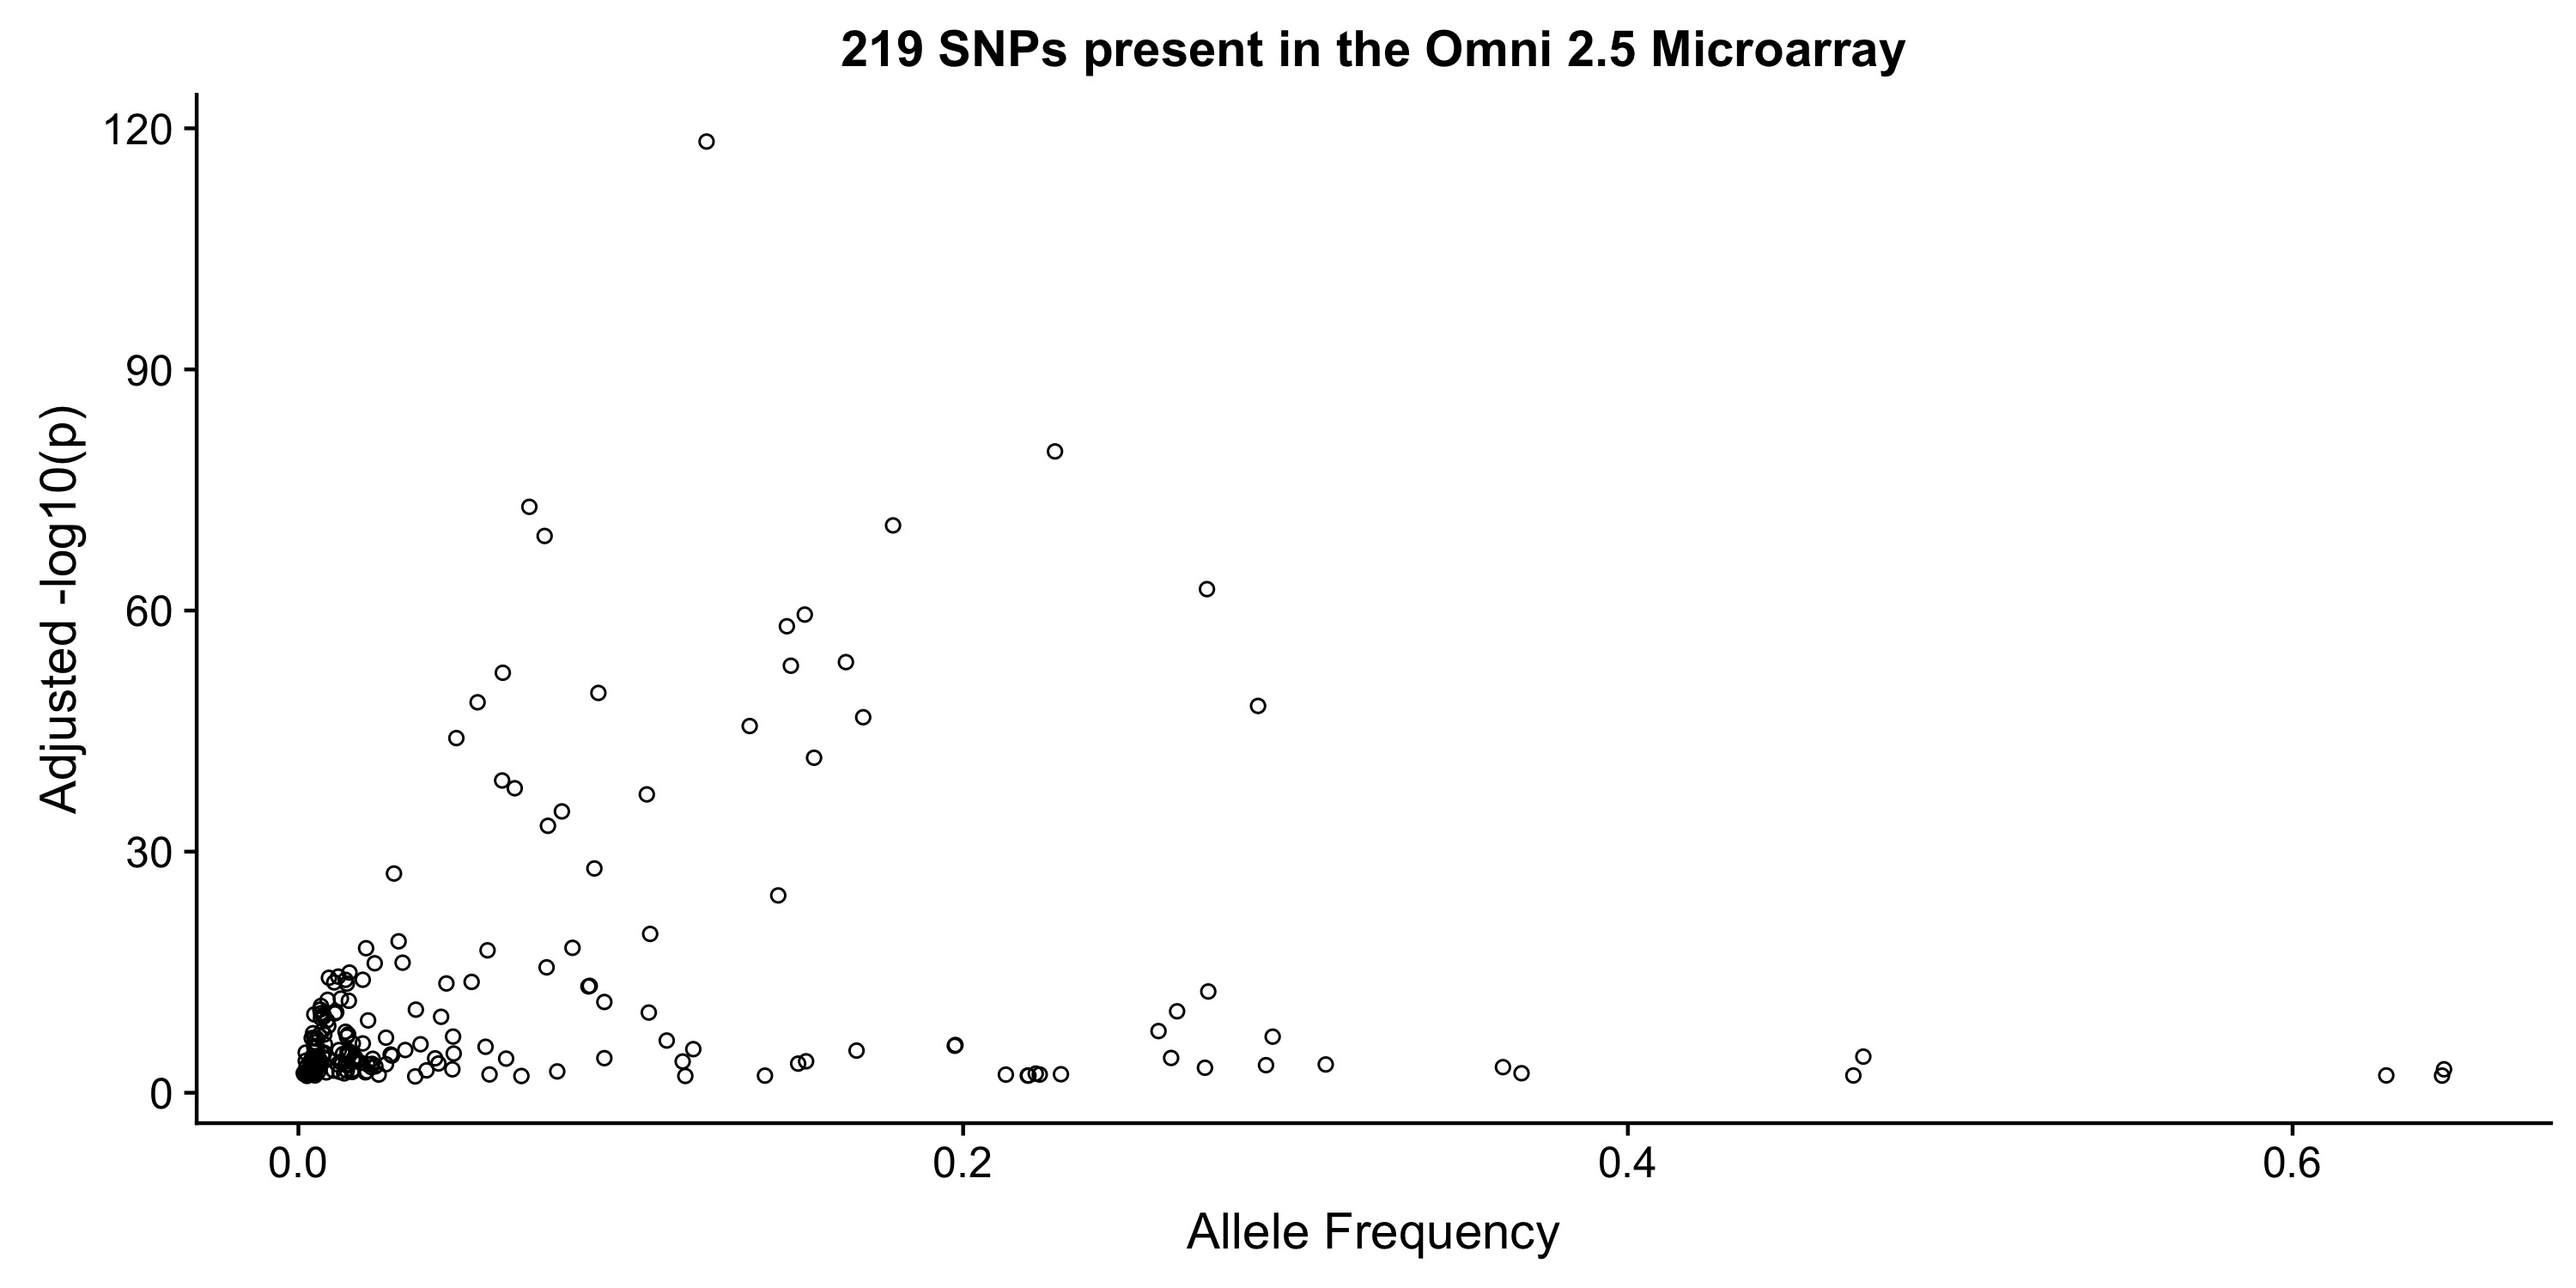
\includegraphics[width=\hsize,keepaspectratio]{./Figures/Omni_AF.jpg}
\caption{We found that 613 of the variants we identified as being associated to $Q$ were present on Illumina's Omni 2.5 chip. 
This does not mean that these variants are false positives, but rather, that in the 1kGP, individuals with low $Q$ were less likely to be called as having a variant in that position. 
Moreover, using the 1kGP as a reference panel might impact the population allele frequencies observed for these positions.}
\label{HapMap_GnomAD}
\end{figure}

\begin{figure}[h]
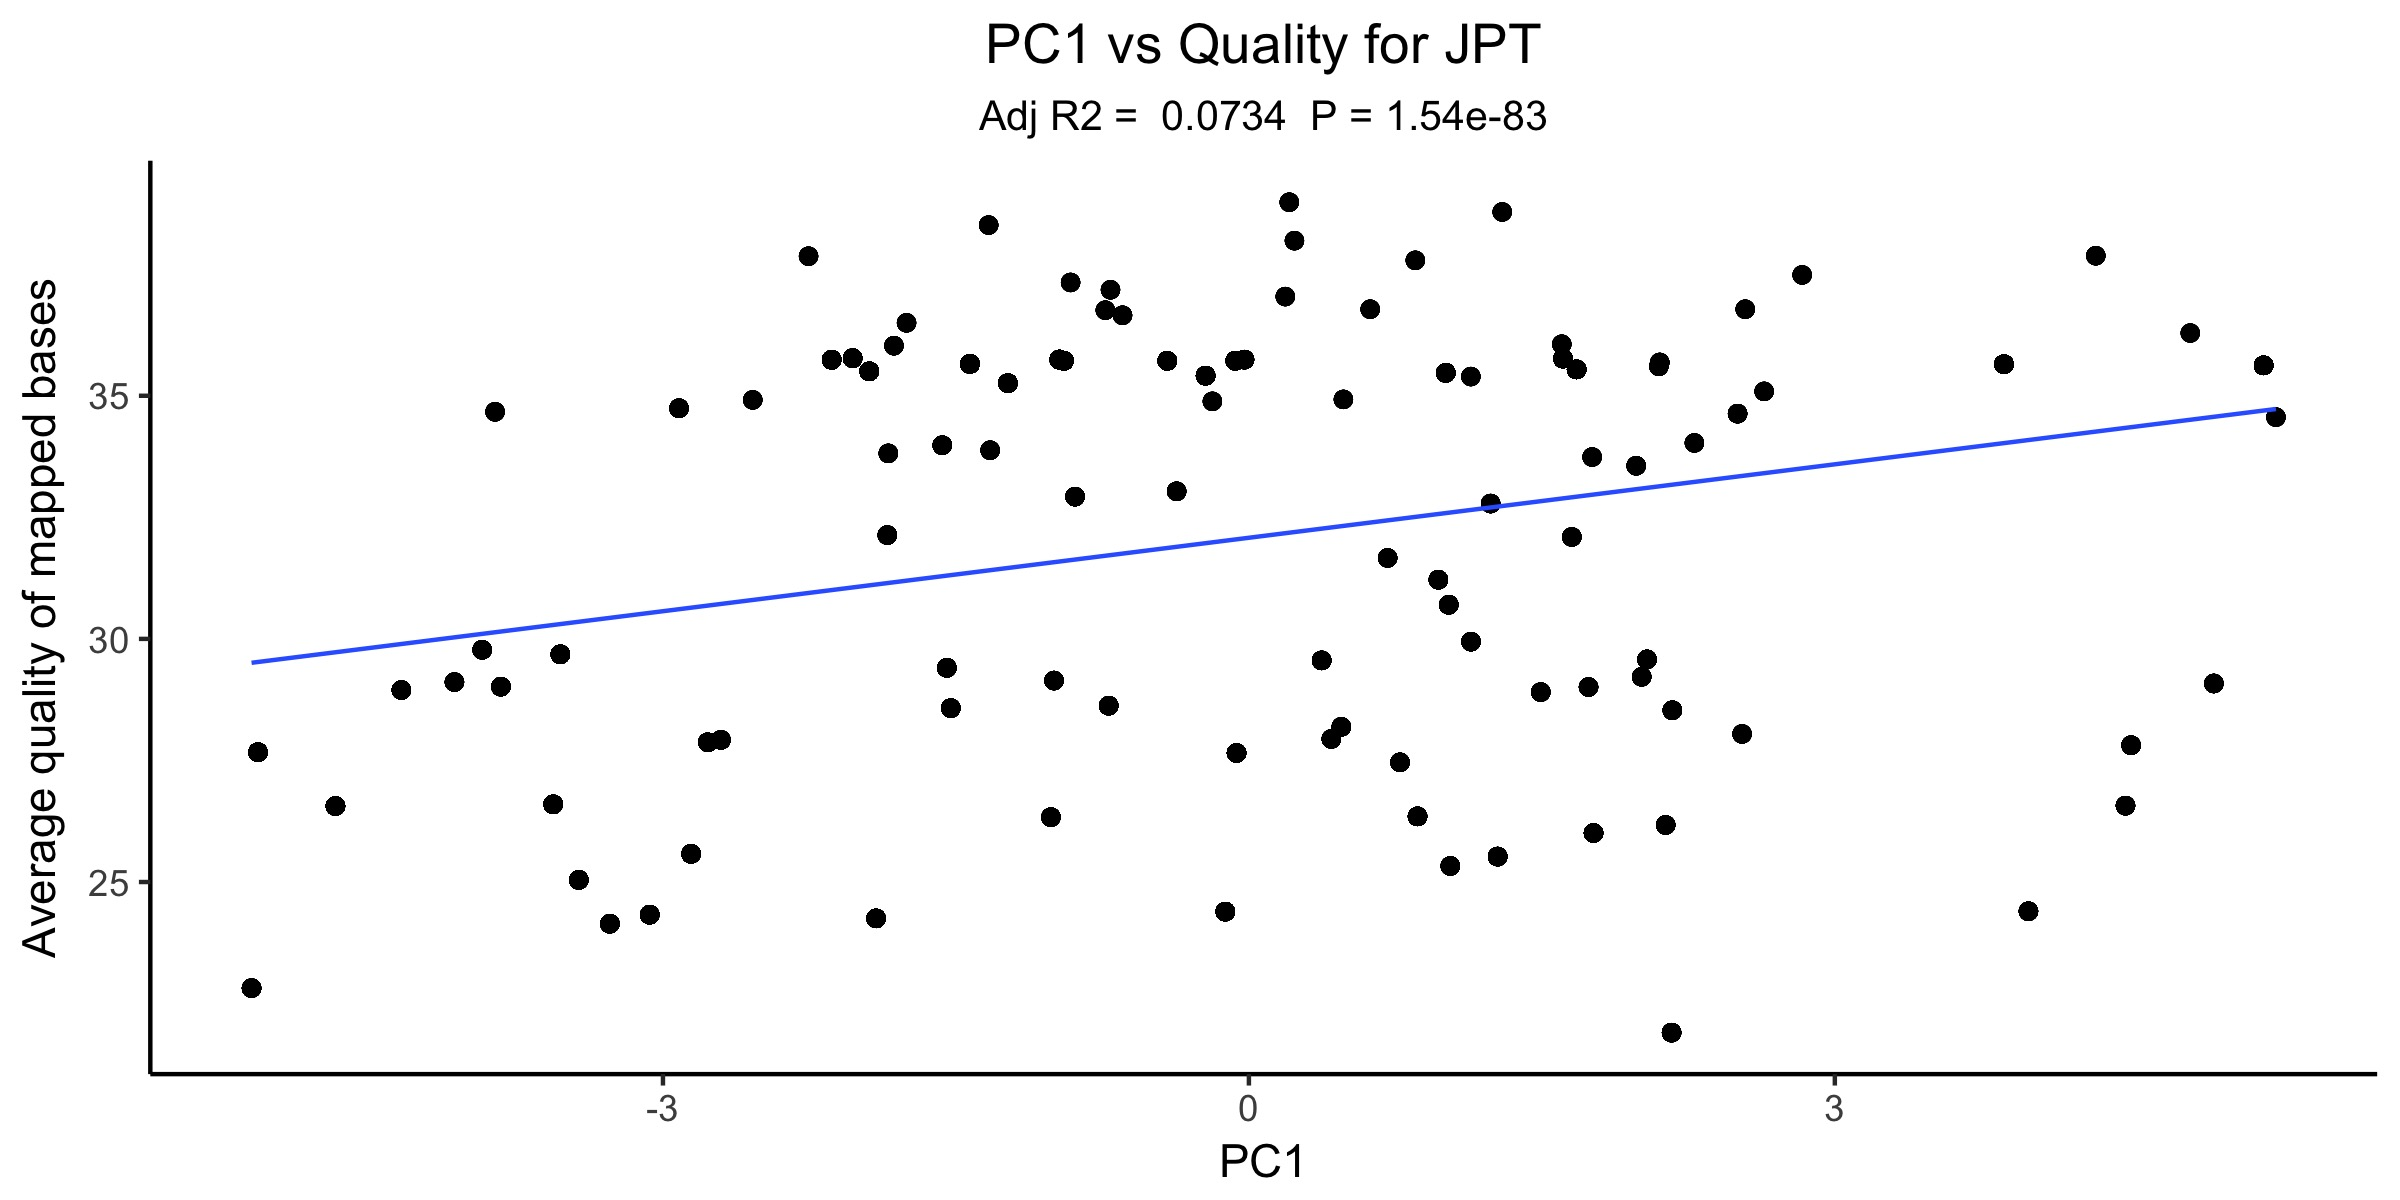
\includegraphics[width=\hsize,keepaspectratio]{./Figures/PC1_Correlation.jpg}
\caption{Plots of data metrics against the prevalence of the  *AC${\rightarrow}$*CC mutational signature in 1kGP. The average quality per mapped bases $Q$ per individual shows some clustering with individuals with low-quality data showing elevated rates of the signature.  }
\label{PC1_Correlation}
\end{figure}

\begin{figure}[h]
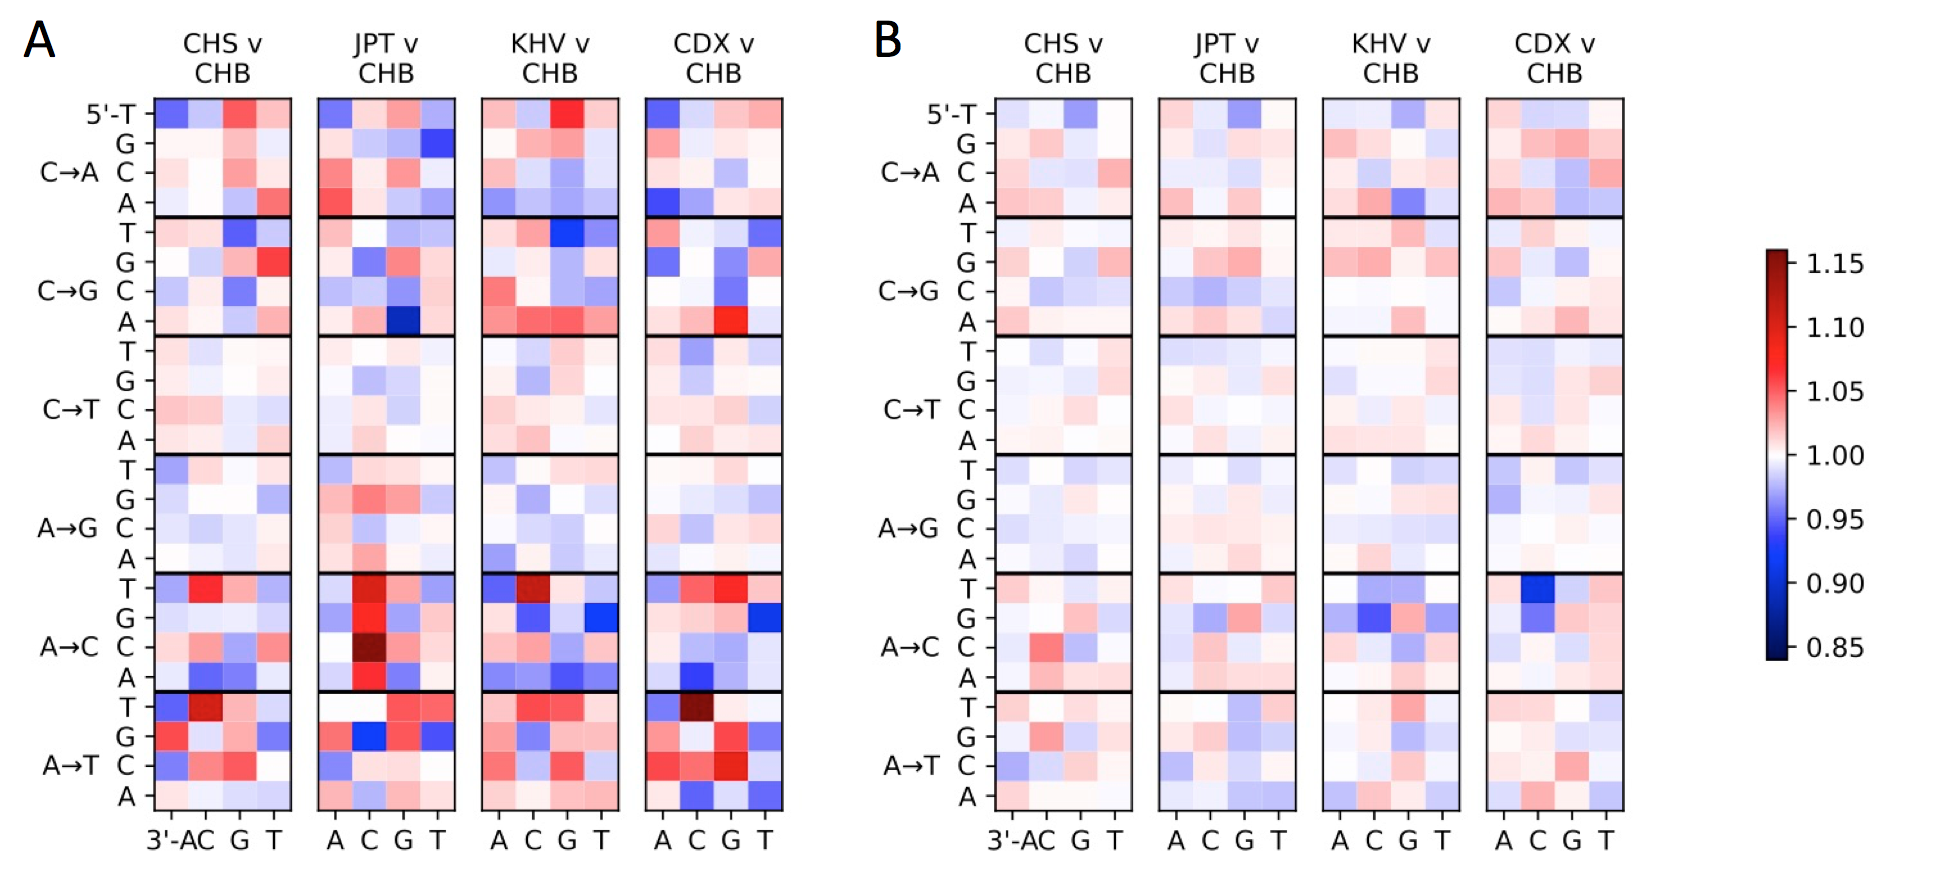
\includegraphics[width=\hsize,keepaspectratio]{./Figures/MutationSpectrum_cutOff.png}
\caption{\textbf{A} 
The  *AC${\rightarrow}$*CC mutational signature in JPT remains despite removing variants associated to quality. 
\textbf{B} 
Removing individuals with average quality per mapped bases $Q$ below a threshold of 30 removes the mutational signature completely. }
\label{MutSpect}
\end{figure}


\end{document}

